\chapter{图像任务的特征学习理论}\label{chap-RBAD}

\section{Introduction}\label{sec-introduction}

Anomalies are rare or suspicious observations that deviate significantly from the pre-defined normal data \cite{DBLP:journals/corr/abs-1901-03407,DBLP:journals/pieee/RuffKVMSKDM21}.
Examples of anomalies include credit card fraud \cite{credit-card-fraud-2011}, defects in manufacturing products \cite{DBLP:journals/ijcv/BergmannBFSS21}, and outbreaks of disease \cite{ourbreaks-of-disease-2023}.
Anomaly detection is a challenging task since negative samples (i.e., anomalies) are hard to obtain at the training stage.
Nevertheless, researchers have developed various anomaly detection methods that require only normal training data.
For example, empirical studies \cite{DBLP:conf/cvpr/SalehiSBRR21,DBLP:journals/corr/abs-2305-15956} have observed an intriguing phenomenon that generative models trained on normal data tend to produce larger reconstruction errors when reconstructing anomalies than normal data.
Accordingly, anomalies can be detected by setting up thresholds for reconstruction errors.
Such anomaly detection methods are referred to as reconstruction-based anomaly detection (RBAD) \cite{DBLP:journals/corr/abs-2305-18593,DBLP:conf/icml/LvSWXX24,DBLP:conf/icml/LiF0CWHSQZ24} in the literature.

Despite the empirical success of RBAD, the theoretical understanding of RBAD is still limited.
A detailed discussion on the related works is postponed to Appendix \ref{sec-related-work} due to limited space.
The main goal of our paper is to establish a theoretical framework for analyzing RBAD and find a plausible explanation for RBAD.
More specifically, we raise the following three research questions.
\begin{itemize}
    \item ($\bm{Q}_1$) \textit{How does the model learn the features from normal training data in RBAD?}
    \item ($\bm{Q}_2$) \textit{What is the role of the learned features in the reconstruction phase?}
    \item ($\bm{Q}_3$) \textit{Why are the anomalies harder to reconstruct compared to normal data?}
\end{itemize}
This paper comprehensively discusses $\bm{Q}_1$ - $\bm{Q}_3$ and provide a brief answer in \ref{sec-conclusion}.

\paragraph{Setup.}
We analyze the training and reconstructing processes of RBADs using tools from \textit{feature learning} \cite{DBLP:conf/focs/Allen-ZhuL21,DBLP:conf/iclr/Allen-ZhuL23};
we refer the readers to Appendix \ref{sec-related-work} for more related works.
Following \cite{DBLP:conf/iclr/Allen-ZhuL23}, we characterize the inputs images as an array of $P$ \textit{patches}.
As illustrated in \ref{fig-different-types-of-anomalies}, patches are small parts of an image that might contain various features and non-feature noise.
In this paper, we adopt the signal-noise data model that characterizes the patches as the sum of a feature and a random noise.
For normal data, the patches contain different features according to some given distribution (cf. \ref{sec-data-assumption}).
We characterize the anomalies as normal data with some of the normal patches replaced by abnormal patches.

We consider a \textit{two-layer convolutional autoencoder} that includes a convolutional hidden layer with max pooling operation.
The network is parameterized by the convolutional kernels $\w$ and is trained by minimizing the empirical reconstruction error using gradient descent with random initialization.
We analyze the training dynamics of the kernels by setting up probability bounds for the growth rates and the magnitude of the kernels.

\paragraph{Theoretical Analysis.}
We quantitatively analyze the training and reconstruction phases of RBADs in \ref{sec-main-results}.
Given feature and iteration step, Definition \ref{def-smost-in-paper} introduces the \textit{cone set} of the feature at that iteration step.
By definition, the ``cones'' would get sharper as iteration steps increase (cf. \ref{fig-geometric-intuition}), which ensures that the kernels in the cone sets would get more aligned to the corresponding feature.
We prove that the cone sets of the features would absorb the kernels during training.
As a result, the absorbed kernels would eventually approximates the features' directions, and by this means, the model extract and learn the features from the training data.
The above analysis provides a plausible answer to question $\bm{Q}_1$.

We answer the questions $\bm{Q}_2$ and $\bm{Q}_3$ by further analyzing the reconstruction phase of RBAD.
Our paper characterizes the anomalies as normal data with some of the normal patches replaced by the abnormal patches.
In \ref{sec-reconstruction}, we study how the learned features process the signal from the input image.
\ref{theorem-small-convolution-in-paper} proves that the processed signal of the abnormal patches would be significantly weaker than those of the normal patches, explaining why the anomalies are hard to reconstruct.

\paragraph{Empirical Validation.}
We conduct experiments on synthesized and real-world datasets to validate the theoretical findings and intuitions.
The setting of the synthesized experiment is identical to our theoretical setting.
As reported in Figure \ref{fig-synthesized-experiment-results}, there is a clear gap between the reconstruction errors of the normal data and the anomalies, which is in consistent with both our theoretical claims and the existing empirical results on RBAD.
We also train networks on real-world anomaly detection datasets and visualize the growth of the kernels in these networks.
The results exhibit clear feature learning processes, which further validate our proposed cone set intuition.

\paragraph{Contribution Statement.}
The main contributions of our paper are summarized as follows.

\begin{enumerate}
    \item We establish a theoretical framework for analyzing RBAD.
The main results and intuitions are summarized in the theoretical roadmap (\ref{fig-theoretical-roadmap}).
Our proposed framework introduces the cone set intuition (Remark \ref{remark-cone-set-intuition} and \ref{fig-geometric-intuition}).
We characterize how neural networks extract features ($\bm{Q}_1$) and reconstruct normal data and anomalies ($\bm{Q}_2$). 
In particular, we prove that a 2-layer convolutional autoencoder trained on normal data cannot accurately reconstruct the anomalies with high probability ($\bm{Q}_3$).

\item We also conduct extensive experiments on synthesized and real-world datasets.
With an identical setting to our theory, the results of the synthesized experiment are consistent with both our theoretical findings and the existing empirical results.
We also visualize the feature learning process on real-world datasets, validating our proposed cone set intuition.
{\color{red} Note that the main goal of our paper is to complement, not compete with, existing RBAD methods. The experiments are mainly conducted to validate our theoretical findings.}
\end{enumerate}

\section{Problem Setup} \label{sec-problem-setup}
Throughout this paper, we denote the vectors by bold letters (e.g., $\x$, $\v$, and $\w$).
The $i$-th entry of $\x$ is noted by $\x^{(i)}$.
For any $N \in \mathbb{Z}^+$, we write $[N] := \{1,2,\cdots, N\}$  and $[\x_{N}] = \{\x : \exists i \in [N]\ s.t.\ \x = \x_i \}$ for simplicity.
The $2$-norm of $\x$ is denoted by $\|\x\|$.
A summarized list of terms and notations is included in Appendix \ref{sec-list-of-terms-and-notations}.

\paragraph{$P$-Patch Data.}
Following \cite{DBLP:conf/iclr/Allen-ZhuL23}, we consider the following {$P$-patch data} ($P \in \mathbb{Z}^+$) model.
As demonstrated in \ref{fig-different-types-of-anomalies}, a patch $\x$ refers to a small part of an image $\z$ that might contain various features (e.g., edges and shapes).
Previous works of feature learning \cite{DBLP:conf/iclr/Allen-ZhuL23,DBLP:journals/corr/abs-2303-04145} characterize the patches as vectors.
In this paper, we let $\H$ be a $d$-dimensional Hilbert space equipped with the inner product $\ip{\x_1,\x_2} := \sum_{i \in [d]} \x_1^{(i)} \cdot \x_2^{(i)}$ for all $ \x_1, \x_2 \in \H$. 
In the rest of this paper, we will call $\x$ a \textit{patch-like vector} if $\x \in \H$.

Real-world images can be split into patches.
Motivated by this, our paper uses disjoint patch-like vectors to represent the images.
More specifically, we say that $\z$ is \textit{$P$-patch data} (or $\z$ has \textit{$P$-patch structure}) if $\z$ can be represented by an array of patch-like vectors, i.e., $\z = (\x_1, \x_2, \cdots ,\x_P)^T \in \H^P$.
For all $ i \in [P]$, we call $\x_i$ a $d$-dimensional \textit{patch} of $\z$. 

Our paper assumes that both the normal data and the anomalies are $P$-patch data with fixed $P$ and $d$. 
In the context of convolutional neural networks, the (convolutional) kernels $\w$ and the patches have identical sizes and shapes. 
Therefore, we assume that the kernels $\w$ are also patch-like vectors.
For all $ \x, \w \in \H$, we call $\ip{\x,\w}$ the \textit{convolution} of $\x$ and $\w$ by convention. 

\paragraph{Features.}
We characterize the features as $d$-dimensional orthogonal patch-like vectors.
Specifically, we assume that the set of all features $\V := \{ \v_1, \v_2,\cdots, \v_d \}$ form an orthonormal basis of $\H$.
Based on whether it is related to the semantic information of the normal data, we further categorize the features into normal and auxiliary features.
As illustrated in \ref{fig-different-types-of-anomalies}, if hand-written digit ``1'' is considered as the normal data, then the patches $\x_{a,1}$, $\x_{a,2}$, $\x_{b,1}$, and $\x_{c,1}$ might contain normal features that capture part of the semantic information of the normal data.
In Figure \ref{fig-different-types-of-anomalies}.c, $\x_{c,2}$ contains an auxiliary feature that captures the semantic information of a semantic anomaly of ``7'' instead of the normal data ``1''.
However, we argue that these auxiliary features can be regarded as either acceptable errors or sample diversity, and thus might appear in normal data with a small yet non-negligible probability.

In this paper, we formalize the collection of normal and auxiliary features of the normal data as disjoint subsets of $\V$, noted by $\V_{nor}$ and $\V_{aux}$, respectively.
Without loss of generality, we assume that $\V_{nor} = \{ \v_1, \v_2\}$ and $\V_{aux} = \{ \v_3, \v_4, \cdots , \v_d  \} $.
Notice that our results can be easily extended to $\V_{nor}$ and $\V_{aux}$ taking arbitrary complementary subsets of $\V$ at the cost of tedious computation.

\begin{figure}[H]
   \begin{center}
   \begin{subfigure}{0.3\columnwidth}
   \centering
   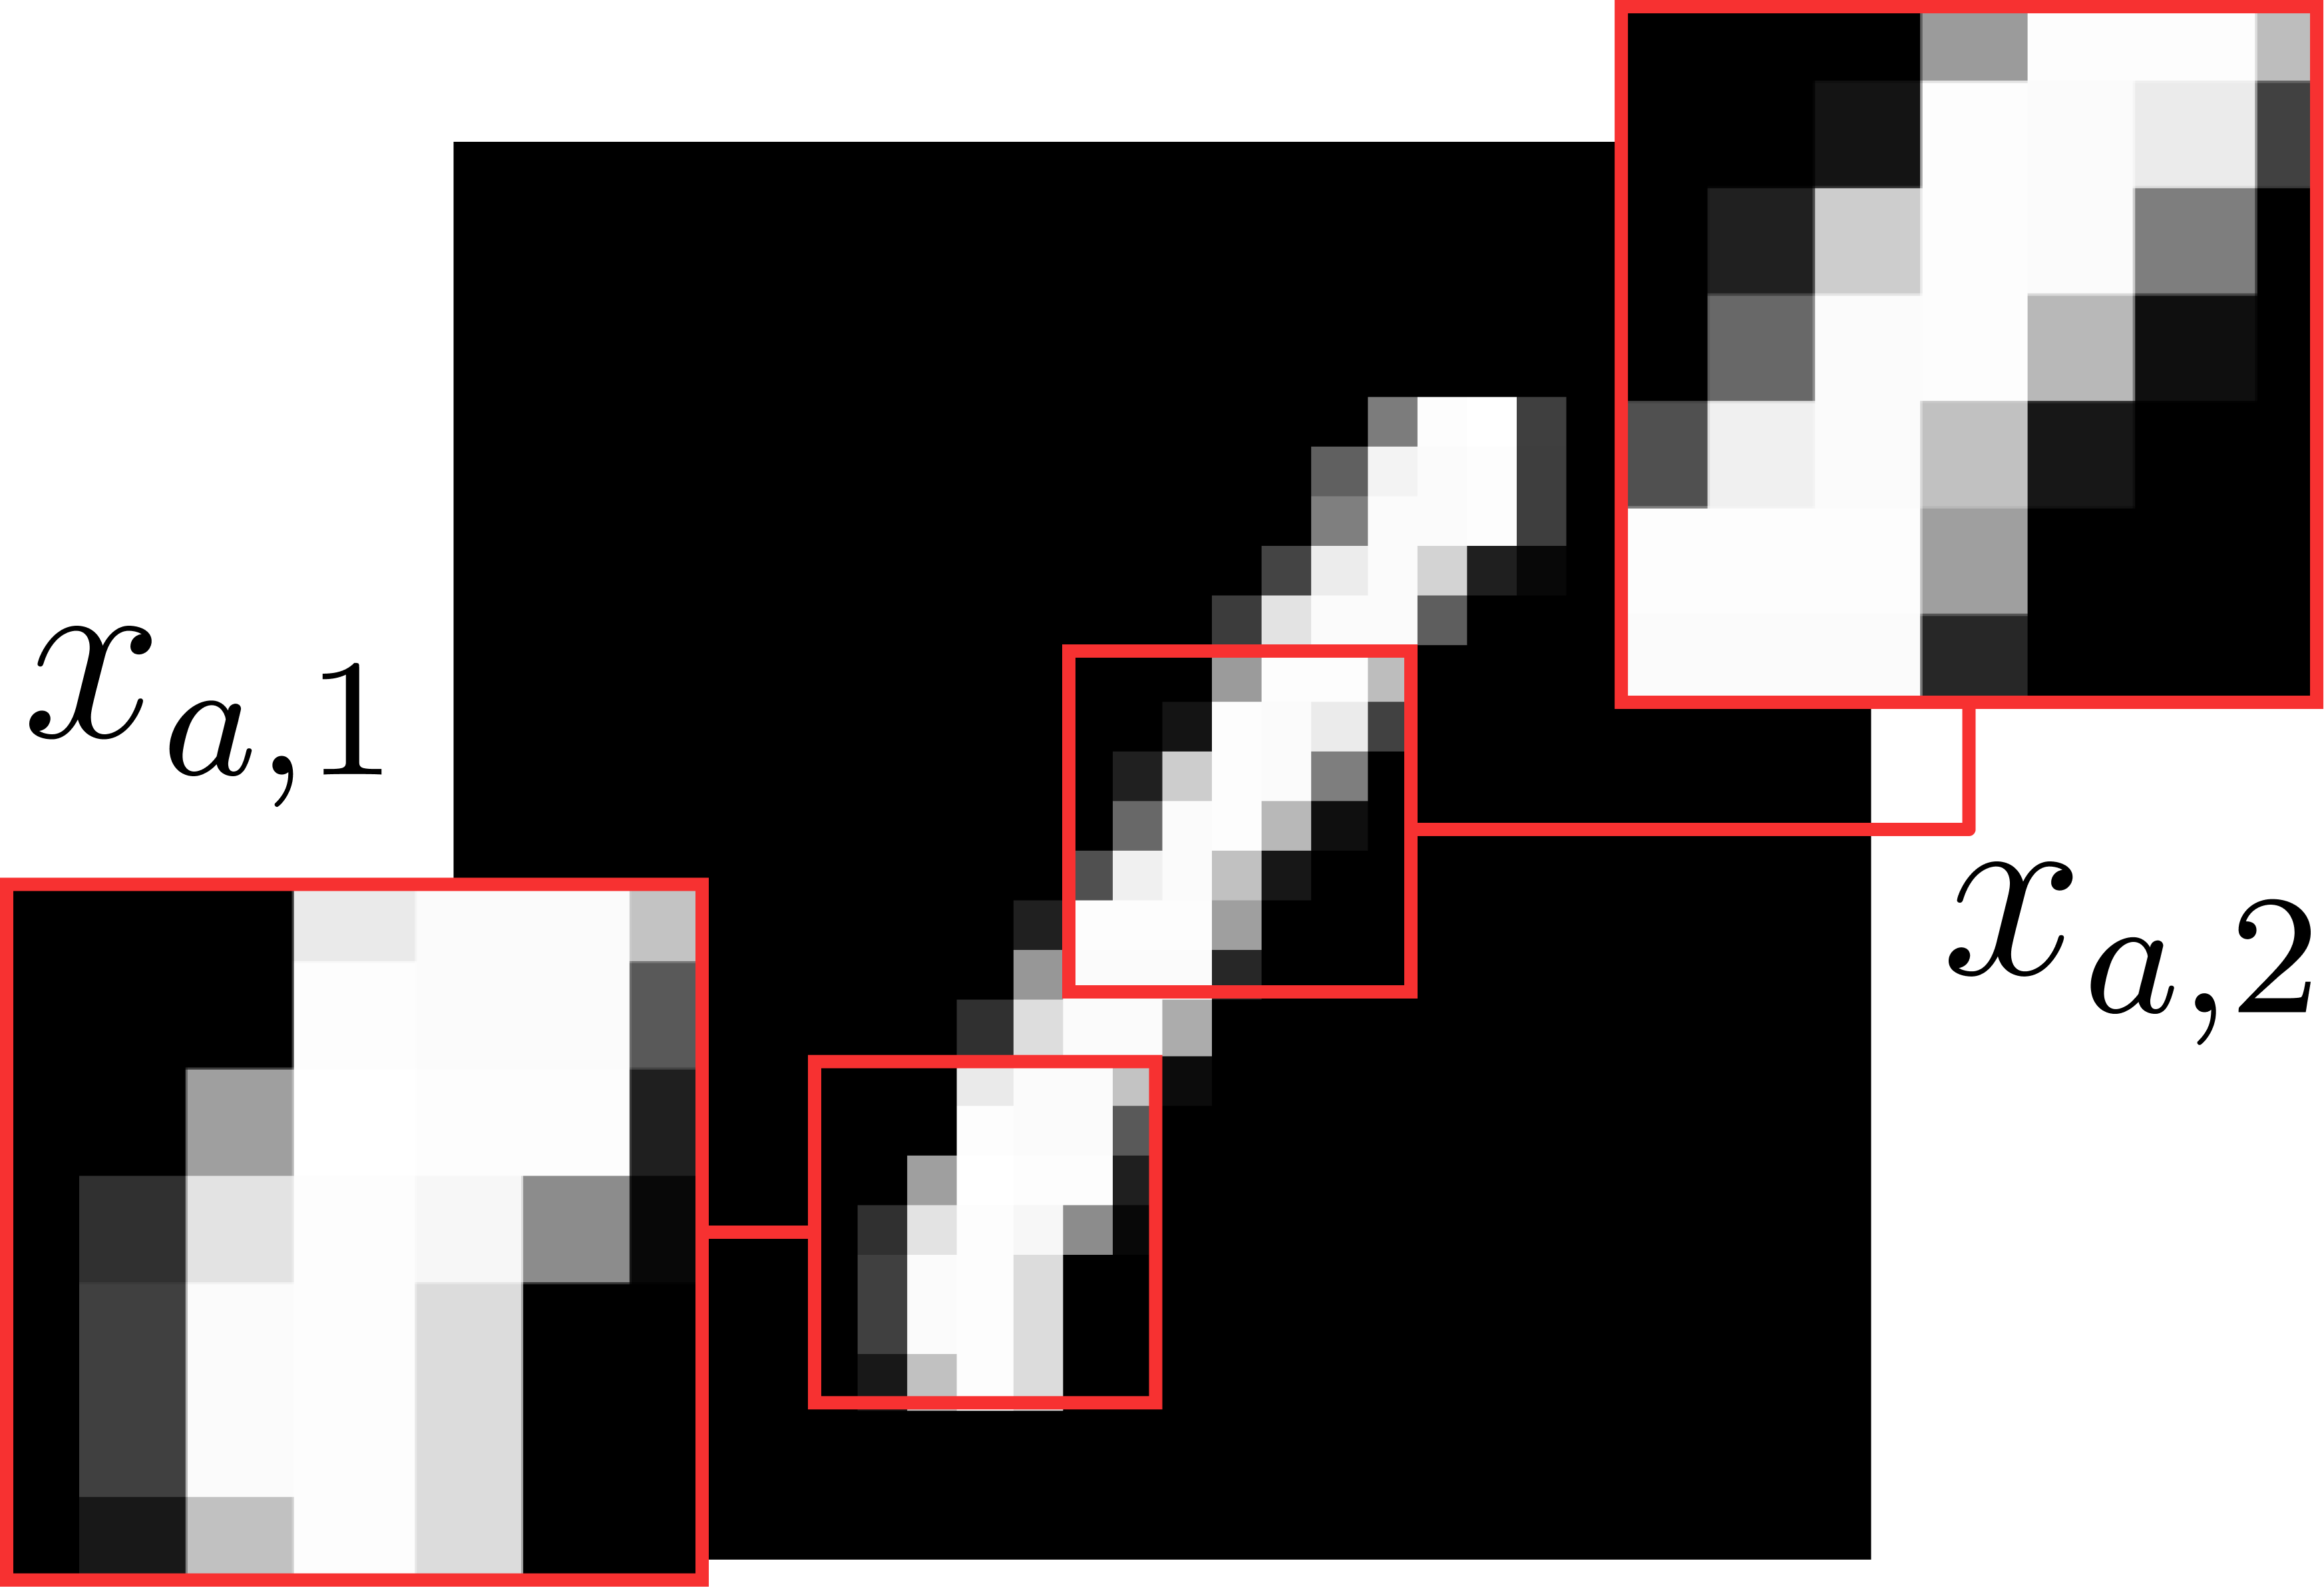
\includegraphics[width=\columnwidth]{figures/rbad/assets/original patch.png}
   \caption{Normal data}
   \label{fig-original-patch}
   \end{subfigure}
   \hfill
   \begin{subfigure}{0.3\columnwidth}
   \centering
   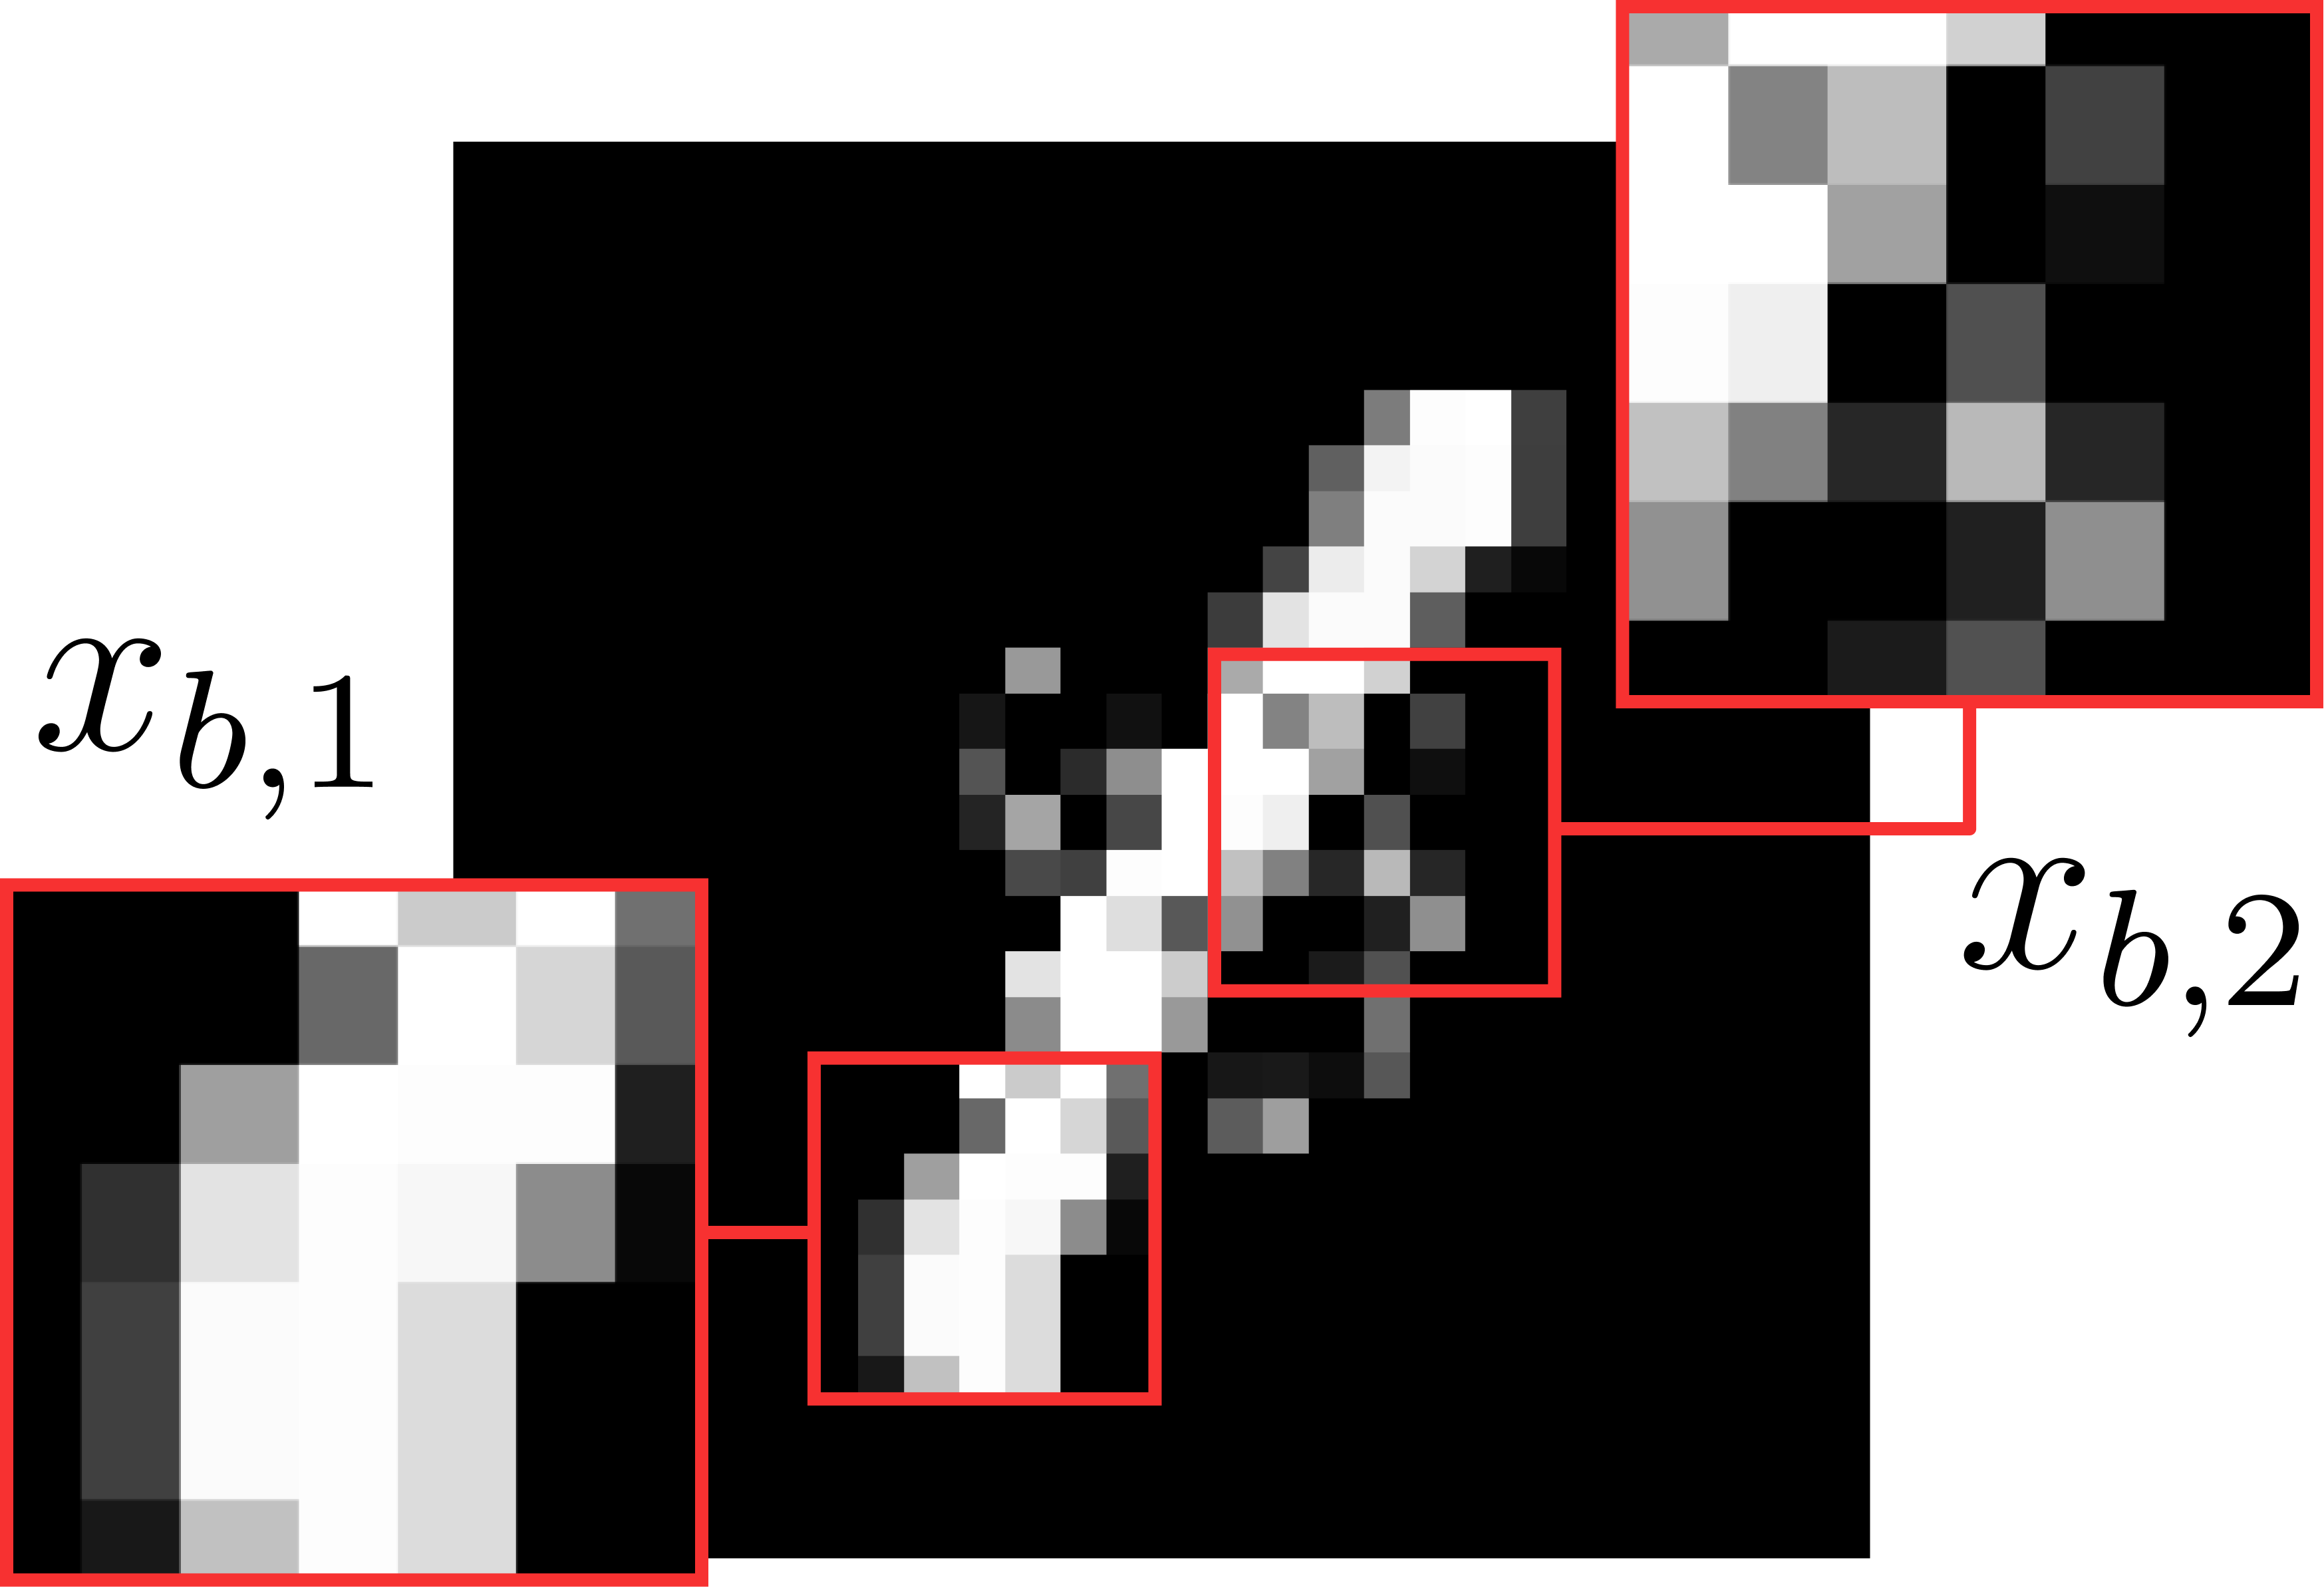
\includegraphics[width=\textwidth]{figures/rbad/assets/sensory anomaly patch.png}
   \caption{Non-semantic anomaly}
   \label{fig-sensory-patch}
   \end{subfigure}
   \hfill
   \begin{subfigure}{0.3\columnwidth}
   \centering
   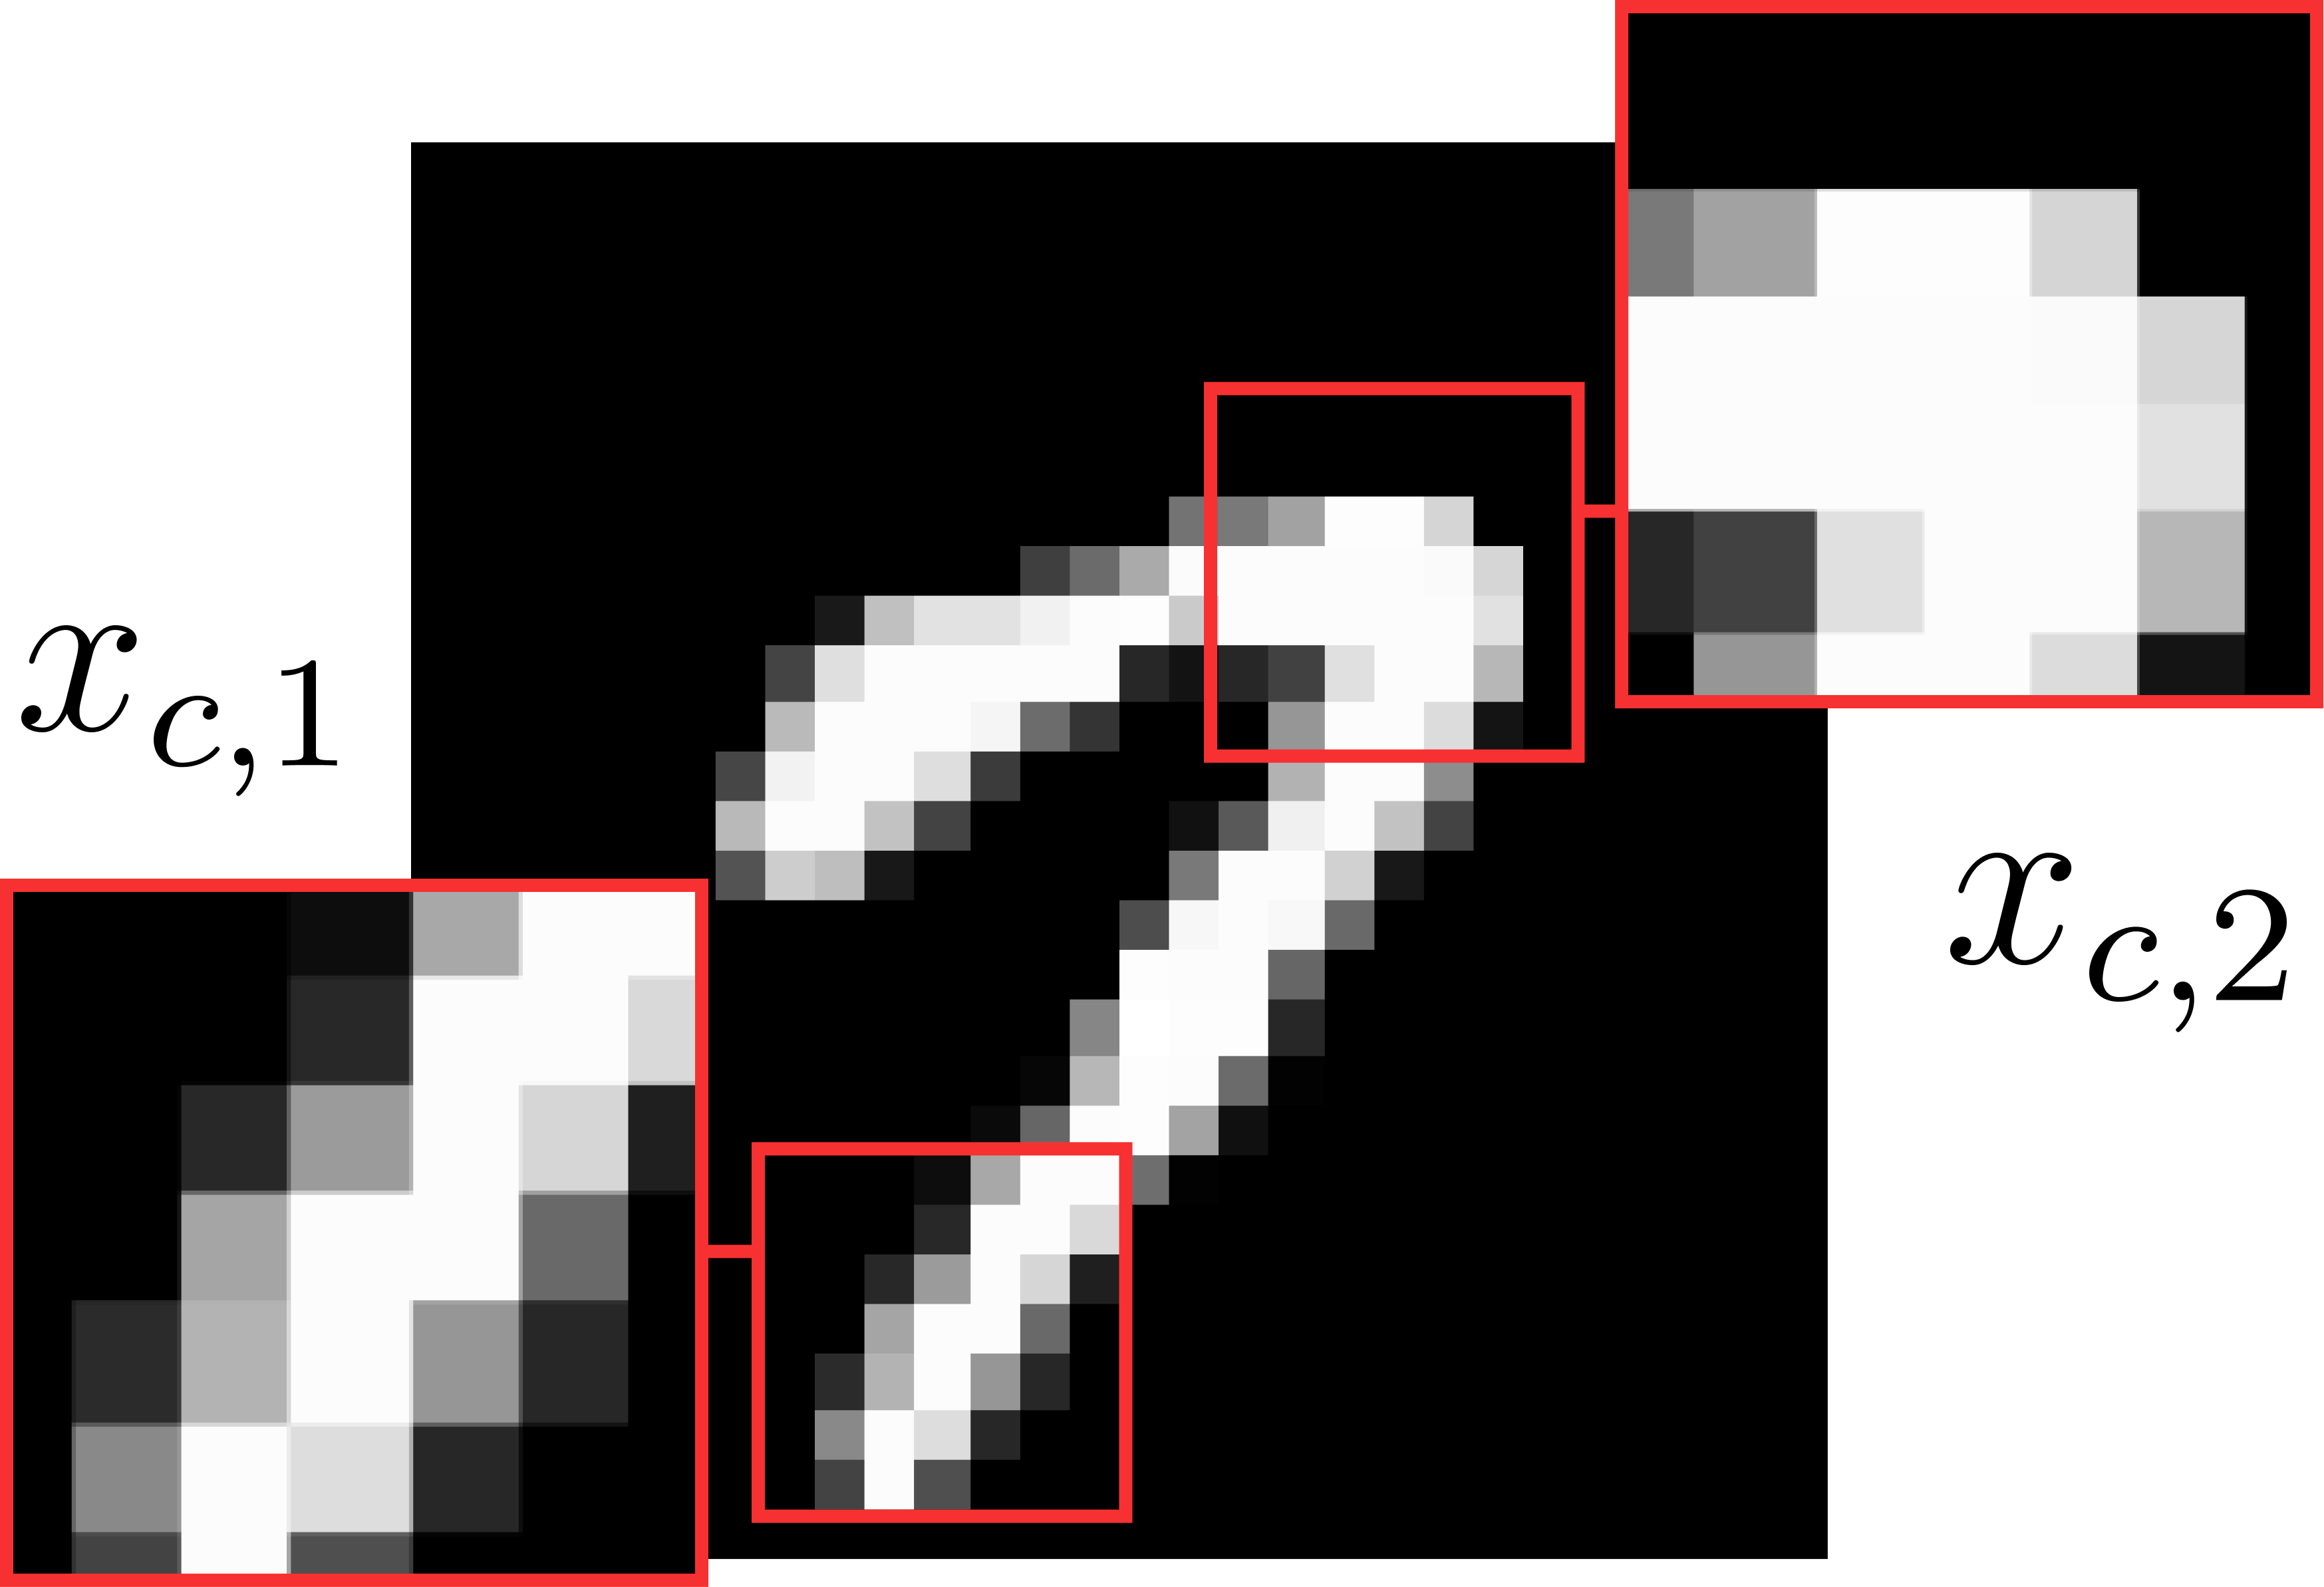
\includegraphics[width=\textwidth]{figures/rbad/assets/semantic anomaly patch.png}
   \caption{Semantic anomaly}
   \label{fig-semantic-patch}
   \end{subfigure}
   \end{center}
   \caption{{
   \textbf{Patches, features, and different types of anomalies}.
   As an illustrative example, consider the handwritten digits with only \qm{1} being normal data.
   Patches $\x$ are small parts of the images, e.g., those outlined with red boxes.
   $\x_{a,1}$, $\x_{a,2}$, $\x_{b,1}$, and $\x_{c,1}$ contain a \textbf{normal feature} that captures the semantic information of \qm{1}.
   \ref{fig-sensory-patch} is called the non-semantic (or sensory) anomaly in the literature since $\x_{b,2}$ contains \textbf{non-feature noise}.
   $\x_{c,2}$ contains an \textbf{auxiliary feature} that does not capture the semantic information of \qm{1}, making \ref{fig-semantic-patch} a semantic anomaly.
   }}
   \label{fig-different-types-of-anomalies}
   \end{figure}

\subsection{Data Distribution}\label{sec-data-assumption}
Our paper assumes that the normal data $\z$ is drawn independently from an implicit distribution $D_{nor}$.
Given normal data $\z$, we assume that each of the patches of $\z$ contains one feature.
Here, we say that a patch $\x_i$ \textit{contains} a feature $\v_k$ if $\x_i = \v_k + \rho$,  in which $\rho$ is a noise term that satisfies $|\langle \rho, \v_k \rangle| \leq \epsilon$ for some given constant $\epsilon > 0$.

For any $k \in [d]$ and $\z \sim \D_{nor}$, we let the probability of the event \{$\exists \x_i \in \z$ such that $\x_i$ contains $\v_k$\} be a given constant $\beta_k \in [0,1]$.
Intuitively, normal data would contain more normal features than auxiliary features.
For simplicity, we assume that $\beta_k = 1$ for all $ k \in \{1,2\}$,
i.e., normal data surely contain normal features.
As for the auxiliary features, we require $\beta_k < 1$ for any $k \in \{ 3,4,\cdots,d \}$ and $\sum_{k^{\prime}=1}^d \beta_{k^{\prime}} = P$ to ensure there is no empty patches.
In summary, we adopt the following assumption for the normal data.
\begin{assumption}[Normal data model]\label{assumption-normal-data}
We assume that normal data $\z = (\x_1, \x_2, \cdots, \x_P)$ is drawn independently from an implicit distribution $D_{nor}$ that satisfies
\begin{enumerate}
    \item for all $i \in [P]$, $\exists k \in [d]$ such that $\x_i$ contains $\v_k$;
    \item for all $k \in [d]$, $\mathbf{P}_{\z \sim \D_{nor}} \left[\exists i \in [P] \mbox{ s.t. } \x_i \mbox{ contains } \v_k\right] = \beta_k$;
    \item $\beta_1 = \beta_2 =1$, $\beta_k < 1$ for all $k \in \{ 3,4,\cdots, d \}$, and $\sum_{k^{\prime}=1}^d \beta_{k^{\prime}} = P$.
\end{enumerate}
\end{assumption}
Given $N \in \mathbb{Z}^+$, let $[\z_N]$ be the training data that is drawn independently from $D_{nor}$, in which $\z_n \in [\z_N]$ is noted by $\z_n := (\x_{n,1}, \x_{n,2}, \cdots, \x_{n,d})$
in the remainder of this paper.
% Note that the anomalies are not considered in the training phase of typical RBADs.
{\color{red}Notably, RBAD does not require anomalies during training, which constitutes one of the core advantages of this method.}
We will introduce the data model for the anomalies later in \ref{sec-reconstruction}.

\subsection{Network Structure}\label{sec-network-structure}
Let $\phi: \H^P \to \H^P$ be a function that reconstructs the inputs.
% One of the main steps of RBAD is to reconstruct the input data. 
It is not hard to show that simple models (e.g., principal component analysis) would fail to reconstruct the normal data due to the unspecified ordering rule of the patches.
Therefore, we use a slightly more sophisticated model, i.e., the 2-layer convolutional autoencoder. 

An autoencoder $\phi$ is composed of an encoder $\phi_e$ and a decoder $\phi_d$, i.e., $\phi(\z) = \phi_d(\phi_e(\z))$ for all $ \z \in \H^P$.
% , i.e., $\phi = \phi_d \circ \phi_e$. 
% Here, $\Z_f$ is a low-dimensional feature space.
Denote the number of channels by $C = c_2 d$ for some given constant $c_2$ and let $\w = (\w_1, \w_2, \cdots, \w_{C})$ be the weight of $\phi_e$, in which $\w_j$ ($j \in [C]$) are kernels as described earlier.
Given input $\z \in \Z$, the output of $\phi_e$ is noted as $\phi_e(\z; \w) = (\phi_e(\z; \w_1), \cdots, \phi_e(\z; \w_C))$, in which
\begin{equation}\label{eq-def-phi-e-entries}
    \phi_e(\z; \w_j) = \left( \sigma(\ip{\w_j,\x_1}), \cdots, \sigma(\ip{\w_j,\x_P}) \right).
\end{equation}
Here, $\sigma(\cdot)$ is the \textit{smoothed ReLU function} defined as
\begin{equation}\label{eq-def-smoothed-relu}
    \sigma(x) = \left\{
    \begin{array}{cl}
        0 & \mbox{if } x \leq 0; \\
        (2c_0)^{-1} x^2&\mbox{if }  0 < x \leq c_0; \\
        x& \mbox{if } x > c_0,
    \end{array}
    \right. 
\end{equation}
for given constant $c_0$.
Unlike the original ReLU function, $\sigma$ is derivable near $0$.
Note that $\phi_e(\z; \w_j)$ is also $P$-patch data, but the dimension of the patch is reduced from $d$ to $1$.

The decoder reconstructs $\z$ according to the features learned by $\phi_e$.
To illustrate how the features are used in construction, consider the following ideal case in which $\w$ perfectly learns the features, i.e., let $C(d) = d$ and $\w_j = \v_j$ for all $ j \in [d]$.
In this case, we can write
\begin{equation}\label{eq-perfect-reconstruction}
    \tilde{\x}_i = \sum_{j \in [d]} \ip{\x_i,\w_j} \w_j = \x_i,
\end{equation}
which provides a trivial yet perfect reconstruction of the patches in $\z$.

We modify the reconstruction in \ref{eq-perfect-reconstruction} by considering an over-parameterized setting with a max pooling operation.
We make these modifications for the following reasons.
First of all, the proof of \ref{theorem-Stk-subset-st+1k} implies that the reconstruction in \ref{eq-perfect-reconstruction} would easily converge to local minima; 
we refer the readers to \ref{remark-overpara-is-necessary} for detailed discussion.
To avoid reaching local minima, we consider an over-parameterized setting with $c_2 > 1$.

In practice, the max pooling operation is placed after the convolution layer to select the most representative patch, i.e., the patch with the maximum convolution value. 
For ease of computation, our work also adds a max pooling operation in the decoder.
For all $ j \in [C]$, let $\delta(i,j)$ be a binary-value function that takes $1$ when 
\begin{equation}\label{eq-def-delta-ij}
        i = \argmax_{i^{\prime} \in [P]} \sigma(\ip{\w_j,\x_{i^{\prime}}})
\end{equation}
and $0$ otherwise.
% \footnote{As discussed in \ref{remark-simplify-delta}, the notation of $\delta(i,j)$ is slightly modified in the proofs after we introduce the training data $\x_{n,i}$ and the iteration step $t$.}. 
Finally, we have the over-parameterized version of \ref{eq-perfect-reconstruction} with max pooling
% A natural extension of \ref{eq-perfect-reconstruction} might be
% \begin{equation}\label{eq-extension-of-perfect-reconstruction}
%     \tilde{\x}_i = \sum_{j \in [C]} a_{i,j} \cdot \sigma( \ip{\w_j, \x_i} ) \w_j,
% \end{equation}
% in which $a_{i,j}$ are parameters.
% However, \ref{eq-extension-of-perfect-reconstruction} introduces too many parameters to the following optimization, making the theoretical analysis hard to proceed. 
% To fix this, we consider
\begin{equation}\label{eq-simplify-extension-of-perfect-reconstruction}
    \phi_d^{(i)} \left(\phi_e(\z) \right) = \sum_{j \in [C]} \sigma(\ip{\w_j,\x_i}) \delta(i,j) \w_j.
\end{equation}
Intuitively, for all $ \x_i \in [\x_P]$, $\phi_d^{(i)} \left(\phi_e(\z) \right)$ reconstructs $\x_i$ by adding together those $\w_j$ such that $\x_i$ is the \qm{most related} patch to $\w_j$.
Combining \ref{eq-def-delta-ij,eq-simplify-extension-of-perfect-reconstruction}, our decoder $\phi_d$ is defined as
\begin{equation}\label{eq-def-phi-d}
\phi_d \left(\phi_e(\z) \right)
= \left( \phi_d^{(1)} \left(\phi_e(\z) \right) , \cdots , \phi_d^{(P)}\left(\phi_e(\z) \right) \right).
\end{equation}
In the rest of this paper, we will always omit the parameter $\w$ if it does not cause confusion.
% \ref{eq-def-phi-e,eq-def-phi-e-entries,eq-def-smoothed-relu,eq-perfect-reconstruction,eq-simplify-extension-of-perfect-reconstruction,eq-def-delta-ij,eq-def-phi-d} give a clear definition of the autoencoder $\phi = \phi_d \circ \phi_e$. 
% We also provide a concrete example of $\phi$ in \ref{appendix-sec-autoencoder} together with several illustrative figures.

\subsection{Training Paradigm}
We train the autoencoder $\phi$ under a standard empirical risk minimization paradigm \cite{DBLP:books/daglib/UML-0033642}.
As mentioned in \ref{sec-data-assumption}, given $N \in \mathbb{Z}^+$, the training data $[\z_{N}]$ are drawn independently from distribution $D_{nor}$.
To measure how well $\phi$ reconstructs the input data, we let the \textit{reconstruction loss} be
\begin{equation}\label{eq-def-loss}
    \ell(\z;\w) = \| \phi(\z;\w) - \z \|^2.
\end{equation}
The corresponding \textit{(empirical) reconstruction error} is defined as $\risk_N(\w) = \frac{1}{N}\sum_{n \in [N]} \ell(\z_n;\w)$.
We minimize $\risk_N(\w)$ using gradient descent with random initialization. 
For all $ j \in [C]$ and $t > 0$, we iterate $\w_j$ by
\begin{equation}\label{eq-def-GD}
    \w^{t+1}_j = \w^t_j - \eta_t \nabla_{\w_j} \risk_N(\w^t)
\end{equation}
for all $ t \in \mathbb{N}$. 
The learning rate $\eta_t$, specified in \ref{sec-parameters}, is a parameter that gradually decreases to $0$ as the iteration step $t$ grows.
Note that $\eta_t$ is independent of $\w_j$.
For all $ j \in [C]$, the random initialization  of $\w_j$ is given by  $\w^{0}_j \sim \N (0,\sigma_0 \I)$, in which $\N(0,\sigma_0 \I)$ is the $d$-dimensional Gaussian distribution and $\sigma_0$ is a given constant.
%%%%%%%%%%%%%%%%%%%%%%%%%%%%%%%%%%%%%%%%%%%%%%%%%%%%%%%%%%%%%%%%%%%%%%%
% Main Results
%%%%%%%%%%%%%%%%%%%%%%%%%%%%%%%%%%%%%%%%%%%%%%%%%%%%%%%%%%%%%%%%%%%%%%%
\section{Theoretical Analysis}\label{sec-main-results}
Our analyses can be roughly divided into two phases: the \textit{training phase} (\ref{sec-training-phase}) and the \textit{reconstruction phase} (\ref{sec-reconstruction}).
The main results and intuitions are summarized in the following theoretical roadmap.
We include a list of summarized terms and notations in \ref{sec-list-of-terms-and-notations}.
The proofs are postponed to \ref{sec-proof}.

\begin{figure}[H]
    \centering
    \includegraphics[width=\textwidth]{figures/rbad/assets/RBAD Theoretical Roadmap.pdf}
    \caption{A \textit{theoretical roadmap} of our analysis. We visualize the dependency of the results and attach a brief explanation for each. We also summarize two major intuitions.}
    \label{fig-theoretical-roadmap}
\end{figure}

% The difference between reconstructing the normal data and the anomalies is discussed in the detection phase.

\subsection{Training Phase}\label{sec-training-phase}

% The central idea of our analysis is that the kernels  by growing fast along the direction of these features.
% In our analyses, the growth rate of the kernels, i.e., $\w_j^{t+1} - \w_j^{t} = -\eta_t \nabla_{\w_j}\risk_N(\w^t)$ is a crucial variable to control.
We start with analyzing the growth of the kernels.
Given $n \in [N]$ and $i \in [P]$, we use
\begin{equation}
\Delta_{n,i} = \x_{n,i} - \phi_d^{(i)} (\phi_e(\z_n))    
\end{equation}
to denote the difference between the input patch $\x_{n,i}$ and its reconstruction $\phi_d^{(i)} (\phi_e(\z_n))$.
Recall that the growth of the kernel is given by $\w_j^{t+1} - \w_j^{t} = -\eta_t \nabla_{\w_j}\risk_N(\w^t)$ in \ref{eq-def-GD}, in which $\nabla_{\w_j}\risk_N(\w^t)$ can be calculated by the following proposition.
\begin{proposition}\label{prop-gradient}
For any $j \in [C]$, the gradient of the empirical reconstruction error is
\begin{equation}\label{eq-prop-gradient-gradient}
\nabla_{\w_j} \risk_N(\w) = - \frac{2}{N} \!  \sum_{n,i} \delta_n(i,j) \left[ \sigma\! \left(\ip{\w_j,\x_{n,i}} \right) \Delta_{n,i} 
+  \ip{\Delta_{n,i}, \w_j} \sigma^{\prime}\!\left(\ip{\w_j,\x_{n,i}} \right) \x_{n,i} \right].
\end{equation}
\end{proposition}
Proposition \ref{prop-gradient} implies a positive correlation between the growth rate of $\w_j$ and 
the size of $\w_j$ (i.e., $\| \w_j\|$), considering that the sizes of $\sigma(\ip{\w_j,\x_{n,i}})$, $\ip{\Delta_{n,i}, \w_j}$, and $\sigma^{\prime}(\ip{\w_j,\x_{n,i}})$ in \ref{eq-prop-gradient-gradient} are all directly related to $\| \w_j \|$. 
The following lemma further controls the initial value and the growth rate of $\|\w_j\|$.
\begin{lemma}\label{lemma-size-of-wj-in-paper}
Let $p_0 = p_0(d)$ and $f_h = f_h(d)$ be parameters.
For all $ j \in [C]$, we have
\begin{equation}\label{eq-lemma-size-of-wj-random-initialization-in-paper}
    \|\w_j^0\| \leq \sigma_0 f_h
\end{equation}
with probability at least $1 - p_0$ with regard to the random initialization of $\w$.
Moreover, for all $ t \in [T]$, the size of $\w_j^t$ is controlled by 
    \begin{equation}\label{eq-lemma-size-of-wj-result-2-in-paper}
        \|\w_j^t\| \leq  t \sigma_0 f_h.
    \end{equation}
    with probability at least $1 - p_0$.
    Here, $T(t,d)$ is a parameter depending on $t$ and $d$.
    % In both \ref{eq-lemma-size-of-wj-random-initialization,eq-lemma-size-of-wj-result-2}, we let $p_0$ take
    % \begin{equation}\label{eq-lemma-size-of-wj-p0}
    %      p_0 = 2\exp \left(- \frac{(f_h - d)^2}{8d}\right).
    % \end{equation}
\end{lemma}

\begin{remark}[\textbf{\textit{Parameter Analysis}}]
Some parameters in this paper, e.g., $p_0$, $f_h$, and $T$, have clear geometrical or probabilistic intuition.
We will explain them in later parts of this paper.
A summary for the parameters can be found in Appendix \ref{sec-list-of-terms-and-notations}.
For simplicity, we will omit the sup- or sub-scripts $t$ and $d$ if it does not cause confusion. 
A set of recommended parameters is given in Appendix \ref{sec-parameters}. \myqed    
\end{remark}

Note that the probability lower bound for \ref{eq-lemma-size-of-wj-random-initialization-in-paper,eq-lemma-size-of-wj-result-2-in-paper} to hold (i.e., at least $1-p_0$) is the same  because, after random initialization, the kernels would grow in a deterministic manner; 
the iteration rule given by \ref{eq-def-GD} introduces no randomness.
The above discussion implies that
those kernels with larger initial values will grow faster.
A simple deduction is that after multiple iterations, the \textit{faster-growing kernels} would take larger values, thus significantly affecting the reconstruction phase of RBAD. 

The following definition introduces the main intuition of our analysis.

% Similarly, we can prove that kernels with a high correlation with the features will also grow faster.
% The following definition specifies a subset of $[\w_{C}]$ that is \qm{most related} to one of the features. 
% The initial value of $\|\w_j\|$ is 
% As discussed in \ref{sec-introduction,sec-related-work}, our analysis is non-asymptotic. The results in our paper include very complicated expressions.
% Therefore, due to limited space, we do not specify the choice of some parameters in this section.
% The choice of parameters is discussed in \ref{sec-remarks}.
\begin{definition}[Cone set]\label{def-smost-in-paper}
    Let $c_1 = c_1(d) \in (0,1)$ and $f_r = f_r(d,t) \leq c_1(d) f_h(d)$ be parameters with $f_r = f_h \cdot o(t)$.
    For any $t \in [T]$ and $k \in [d]$, let the cone set of feature $\v_k$ at iteration $t$, denoted by $\smost^t(k)$, be the collection of $\w_j \in [w_C]$ such that
\begin{itemize}
    \item $ \ip{ \w_j^{t} , \v_{k} } \geq t \sigma_0 c_1 f_h $, and
    \item for any $k^{\prime} \neq k $, $ \ip{ \w_{j}^{t} ,  \v_{k^{\prime}} } \leq t \sigma_0 f_r $.
    % \item $\| \w_j \| \leq (c_1 - c_2) (\sqrt{2\epsilon})^{-1} \eta_t \sigma_0 \sqrt{ \log d }$
\end{itemize}
We say that kernel $\w_j$ is \textbf{absorbed} by the cone sets of feature $\v_k$ if $\exists t_0 \in [T]$ such that $\w_j^t \in \smost^{t}(k)$ for all $t \geq t_0$, i.e., after the iteration step $t_0$, the kernel $\w_j$ is always in the cone set of feature $\v_k$.
\myqed
\end{definition}

\begin{remark}[\textbf{\textit{Cone Set Intuition}}]
\label{remark-cone-set-intuition}
For any $k \in [d]$ and $t \in [T]$, $k$, $t$ together with the parameters $\sigma_0$,  $c_1$, $f_h$ and $f_r$ specify a $d$-dimensional hypercone with height $t \sigma_0 c_1 f_h$ and radius $t \sigma_0 f_r$.
According to Definition \ref{def-smost-in-paper}, those $\w_j^t \in \smost^{t}(k)$ are bounded by the surface of the cone.
Since we let $f_r = f_h \cdot o(t)$, the cone would get sharper during training (cf. \ref{fig-geometric-intuition}).
As a result, the kernels in the cone would get more aligned to feature $\v_k$.
In particular, the kernels absorbed by the cone set of a feature will eventually approximate to the direction of that feature.
\myqed
\end{remark}

We can obtain the following lemma directly from Definition \ref{def-smost-in-paper}.
\begin{lemma}\label{lemma-smost-delta-ij-in-paper}
    For all $ t \geq 1$, if $j \in \smost^t(k)$ and $\x_i$ contain $\v_k$, then we have $\delta(i,j) = 1$.
\end{lemma}
% The good properties of $\smost$ would greatly simplify the analysis of the training process of $\phi$.
Lemma \ref{lemma-smost-delta-ij-in-paper} implies that the kernels in the cones of a feature $\v_k$ will contribute to the reconstruction of the patches that contain $\v_k$ at all iterations.
Lemma \ref{lemma-smost-delta-ij-in-paper} also simplifies the iteration analysis for the kernels in the cones.
We can prove the following theorem with the help of Lemmas \ref{lemma-size-of-wj-in-paper} and \ref{lemma-smost-delta-ij-in-paper}.

\begin{theorem}\label{theorem-Stk-subset-st+1k}
    For all $k \in [d]$, if $|\smost^{0}(k)| \geq 1$, then $\smost^{t}(k) \subseteq \smost^{t+1}(k)$ for all $t \in [T]$.
\end{theorem}

\begin{remark}[\textbf{\textit{Interpretation of \ref{theorem-Stk-subset-st+1k}}}]
\ref{theorem-Stk-subset-st+1k} characterizes how the kernels of the autoencoder extract features from the training data, providing an answer for question $\bm{Q}_1$.
For all $k \in [d]$ and $t \in [T]$, \ref{theorem-Stk-subset-st+1k} implies that $\w_j \in \smost^t(k)$ will keep growing faster along $\v_k$ than along $\v_{k^{\prime}}$ for all $ k^{\prime} \neq k$.
The geometrical intuition is that \textit{the kernel will be absorbed by the cone set of a feature if it comes into the cone set once}.
After multiple iterations, $\langle \w_{j}^{t} ,  \v_{k^{\prime}} \rangle$ would become almost negligible compared to $ \langle  \w_j^{t} , \v_{k} \rangle$ since $f_r = f_h \cdot o(t)$.
The direction of $\w_j$ gradually approximates to the direction of $\v_k$ as $t$ increases, i.e., $\w_j$ learns the direction of $\v_k$.
\end{remark}

For any $ k \in [d]$, the following theorem proves that $\smost(k)^{0}$ is not empty with high probability.
\begin{theorem}\label{theorem-initial-size-in-paper}
Let $p_1 = p_1(d)$ and $p_2 = p_2(d)$ be parameters.
For all $ k \in [d]$, the size of $\smost^0(k)$ can be upper-bounded by
\begin{equation}\label{eq-lemma-init-prob-smost-result-upper-bound}
     | \smost^0(k) |  \leq C p_2 + \lambda,
\end{equation}
with probability at least $ 1 - \exp\left( - \frac{3\lambda^2}{6C p_2 + 2\lambda} \right)$ over random initialization.
The lower-bound
\begin{equation}\label{eq-lemma-init-prob-smost-result-lower-bound}
    | \smost^0(k) | \geq C p_1 - \lambda
\end{equation}
hold with probability at least $1 - \exp \left( - \frac{\lambda^2}{2 C p_2} \right)$.
\end{theorem}

Theorems \ref{theorem-Stk-subset-st+1k} and \ref{theorem-initial-size-in-paper} together characterize the growth of the kernels $\w_j$ in the cones of the features.
\ref{fig-geometric-intuition} demonstrates the geometric intuition of our results. 

\begin{figure}[H]
    \centering
    \begin{subfigure}{0.32\columnwidth}
    \centering
    \begin{tikzpicture}[tdplot_main_coords]
    % Draw axes
    \draw[->] (0,0,0) -- (2,0,0) node[anchor=north east]{ $\v_1$ };
    \draw[->] (0,0,0) -- (0,2,0) node[anchor=north west]{$\v_2$};
    \draw[->] (0,0,0) -- (0,0,2) node[anchor=south]{$\v_3$};
    \draw[dashed] (-1,0,0) -- (0,0,0) ;
    \draw[dashed] (0,-1,0) -- (0,0,0) ;
    \draw[dashed] (0,0,-1) -- (0,0,0) ;

    \draw[fill=blue!40, , opacity=0.3] (0,0,0) -- plot[variable=\t,domain=-40:115] ({0.2*cos(\t)}, {0.2*sin(\t)}, {0.2}) -- cycle;
    \draw[fill=blue!40, , opacity=0.3] (0,0,0) -- plot[variable=\t,domain=115:212] ({0.2*cos(\t)}, {0.2*sin(\t)}, {0.2}) -- cycle;
    \draw[fill=blue!40, , opacity=0.3] (0,0,0) -- plot[variable=\t,domain=212:320] ({0.2*cos(\t)}, {0.2*sin(\t)}, {0.2}) -- cycle;

    \draw[->] (0,0,0) -- ({0.4*cos(70)}, {0.3*sin(70)}, {0.2}); 
    \node[anchor=west] at (0.3,0.5,0.25) {$\w_{j_1}$};
    \draw[->] (0,0,0) -- ({0.1*cos(270)}, {0.1*sin(270)}, {0.2}); 
    \node[anchor=center] at (0.3,-0.5,-0.05) {$\w_{j_2}$};

    \end{tikzpicture}
    \caption{{At initialization ($t = 0$)}}
    \label{fig-geometric-intuition-1}
    \end{subfigure}
    \hfill
    \begin{subfigure}{0.32\columnwidth}
    \centering
    \begin{tikzpicture}[tdplot_main_coords]
    % Draw axes
    \draw[->] (0,0,0) -- (2,0,0) node[anchor=north east]{$\v_1$};
    \draw[->] (0,0,0) -- (0,2,0) node[anchor=north west]{$\v_2$};
    \draw[->] (0,0,0) -- (0,0,2) node[anchor=south]{$\v_3$};
    \draw[dashed] (-1,0,0) -- (0,0,0) ;
    \draw[dashed] (0,-1,0) -- (0,0,0) ;
    \draw[dashed] (0,0,-1) -- (0,0,0) ;

    \draw[fill=blue!40, opacity=0.3] (0,0,0) -- plot[variable=\t,domain=-40:115] ({0.23*cos(\t)}, {0.23*sin(\t)}, {0.6}) -- cycle;
    \draw[fill=blue!40, opacity=0.3] (0,0,0) -- plot[variable=\t,domain=115:212] ({0.23*cos(\t)}, {0.23*sin(\t)}, {0.6}) -- cycle;
    \draw[fill=blue!40, opacity=0.3] (0,0,0) -- plot[variable=\t,domain=212:320] ({0.23*cos(\t)}, {0.23*sin(\t)}, {0.6}) -- cycle;

    \draw[->] (0,0,0) -- ({0.2*cos(270)}, {0.2*sin(270)}, {0.8});     \node[anchor=center] at (-0.5,-0.8,0.9) {$\w_{j_2}$};
    \draw[->] (0,0,0) -- ({0.2*cos(165)}, {0.2*sin(165)}, {0.8});     \node[anchor=center] at (0,0.5,1.1) {$\w_{j_1}$};

    \end{tikzpicture}
    \caption{{After multiple steps}}
    \label{fig-geometric-intuition-2}
    \end{subfigure}
    \hfill
    \begin{subfigure}{0.32\columnwidth}
    \centering
    \begin{tikzpicture}[tdplot_main_coords]
    % Axes
    \draw[->] (0,0,0) -- (2,0,0) node[anchor=north east]{$\v_1$};
    \draw[->] (0,0,0) -- (0,2,0) node[anchor=north west]{$\v_2$};
    \draw[->] (0,0,0) -- (0,0,2) node[anchor=south]{$\v_3$};
    \draw[dashed] (-1,0,0) -- (0,0,0) ;
    \draw[dashed] (0,-1,0) -- (0,0,0) ;
    \draw[dashed] (0,0,-1) -- (0,0,0) ;

    \draw[fill=blue!40, opacity=0.3] (0,0,0) -- plot[variable=\t,domain=-40:115] ({0.25*cos(\t)}, {0.25*sin(\t)}, {1.7}) -- cycle;
    \draw[fill=blue!40, opacity=0.3] (0,0,0) -- plot[variable=\t,domain=115:212] ({0.25*cos(\t)}, {0.25*sin(\t)}, {1.7}) -- cycle;
    \draw[fill=blue!40, opacity=0.3] (0,0,0) -- plot[variable=\t,domain=212:320] ({0.25*cos(\t)}, {0.25*sin(\t)}, {1.7}) -- cycle;

    \draw[->] (0,0,0) -- ({0.2*cos(270)}, {0.2*sin(270)}, {1.8});     \node[anchor=center] at (-0.1,-0.8,1.4) {$\w_{j_2}$};
    \draw[->] (0,0,0) -- ({0.2*cos(165)}, {0.2*sin(165)}, {1.8});     \node[anchor=center] at (0,0.8,1.6) {$\w_{j_1}$};
    
    \end{tikzpicture}
    \caption{At convergence}
    \label{fig-geometric-intuition-3}
    \end{subfigure}
    \caption{\textbf{The geometry intuition for \ref{theorem-initial-size-in-paper,theorem-Stk-subset-st+1k}.}
    Consider $d = 3$ and $\w_{j_1},\w_{j_2} \in \smost(3)^0$.
    The kernels are absorbed in the cone represented by the light blue surface.
    Definition \ref{def-smost-in-paper} implies that the cone would get sharper as $t$ increases. 
    \ref{theorem-Stk-subset-st+1k} proves that $\w_{j_1}, \w_{j_2}$ will be absorbed if $\w_{j_1},\w_{j_2} \in \smost(3)^0$.
    \ref{theorem-initial-size-in-paper} implies that the cone set is non-empty with high probability.
    }
    \label{fig-geometric-intuition}
\end{figure}

It is worth mentioning that the above results hold for all feature $\v_k$ with $\beta_{k} \neq 0$, regardless of whether $\v_k$ is a normal feature or an auxiliary feature.
Recall that we use auxiliary features to characterize patterns not directly related to the semantics of the normal data.
As a minor implication, we prove that neural networks would also learn the auxiliary features.
The following corollary discusses the tightness of the bounds for different features.

\begin{corollary}[Informal]\label{corollary-cone}
Recall that \ref{def-smost-in-paper} implies a growth rate gap between the kernels growth along the ``cone feature's direction'' and other features direction.
For those kernels absorbed in the cones of normal features, the growth rate gap is larger than those in auxiliary features.
\end{corollary}

The formal version of this corollary is postponed to Appendix \ref{sec-proof} due to limited space.

In summary, this section analyzes the training phase of RBADs.
Notice that the question $\bm{Q}_1$ is answered in this section.
It remains to discuss how the features are used in the reconstruction phase and why the anomalies are hard to reconstruct.

\subsection{Reconstruction Phase}\label{sec-reconstruction}
Since the learning rate $\eta_t$ decreases to $0$ as $t$ grows, the kernels would gradually converge. 
Denote the converged kernels by $\w^{*}:= (\w^*_1, \w^*_2, \cdots, \w^*_P)$ and the corresponding network by $\phi^{*}$.
\ref{sec-reconstruction} discusses how $\phi^{*}$ reconstruct the input images.

We start by introducing the data model for anomalies.
% discussing the non-semantic anomalies.
Let $\z \sim D_{nor}$ be normal data (cf. Assumption \ref{assumption-normal-data}) and $\x_a \in \H$ be a patch.
Given $i_0 \in [P]$,
% we say that a $P$-patch data is if one of its patches is replaced by another patch-like vector that does not contains a feature.
% More specifically, we assume that $\exists \x_a \in \H$ and $\| \x_a \| \in [1-\epsilon,1+\epsilon]$. 
the \textit{anomaly} is defined as 
\begin{equation}\label{eq-def-anomalies}
    \z(i_0,\x_a) := (\x_1, \cdots, \x_{i_0-1},\x_a, \x_{i_0+1}, \cdots, \x_P),
\end{equation}
i.e., one of the patches in $\z$ is replaced by $\x_a$.
We call $\z(i_0,\x_a)$ a \textit{semantic anomaly} if $\exists k \in [d]$ such that $\x_a$ contains $\v_k$ and a \textit{non-semantic anomaly} if otherwise.
For non-semantic anomalies, we further assume that $\x_a$ is drawn from the uniform distribution supported on $\{\x : \|\x\| = 1\}$.
% In other words, we assume that the non-semantic anomalies are average data with one of its patches being replaced by another patch-like vector that does not necessarily contain a feature.
Note that our analysis can be trivially extended to the case where multiple patches are replaced.

In order to answer $\bm{Q}_2$, we go on to analyze the behavior of the kernels in the reconstruction phase.
Taking $\z(i,\x_a)$ as the input of $\phi^*$, by definition, we have
\begin{equation}
    \phi_e^{(i)}(\z(i_0,\x_a); \w^{*}_j) = \sigma(\ip{\w_j, \x_i}) = \phi^{(i)}_e(\z; \w^{*}_j)
\end{equation}
for all $ i \in [P]$ such that $i \neq i_0$.
% We first discuss the non-semantic anomalies.
Since $\V$ is an orthonormal basis of $\H$, we can decompose $\x_a$ as 
\begin{equation}\label{eq-xa-decomposition}
    \x_a = \sum_{k \in [d]} \ip{\x_a,\v_k} \v_k.
\end{equation}
By taking \ref{eq-xa-decomposition} into \ref{eq-def-phi-e-entries}, the replaced patch is encoded as follows.
\begin{equation}
    \phi_e^{(i_0)}(\z(i_0,\x_a); \w^{*}_j) 
    =  \sigma(\ipsmall{\w_j^*, \sum_{k \in [d]} \ip{\x_a,\v_k} \v_k}) 
    = \sigma( \sum_{k \in d} \ip{\x_a,\v_k} \ip{\w_j^*,\v_k} ).
\end{equation}
For all $ j \in [C]$, by definition, the max pooling operation only reserves $\max_{i \in [P]} \sigma(\langle \w_j,\x_i \rangle)$.
We have proved in \ref{sec-training-phase} that the direction of the kernels would gradually get closer to the directions of the features.
% However, \ref{theorem-main-in-paper} proves that the kernels would stay in the cones of the features. 
For non-semantic anomalies, we can prove the following theorem.
\begin{theorem}\label{theorem-small-convolution-in-paper}
    For all $ \theta \in (0,1)$, $\forall j \in [C]$, and $\forall k \in [d]$, if $\ip{\w_j, \v_k} > (1 - \theta)\cdot \|\w_j\|$, then
    \begin{equation}
        \ip{{\w_j}, \x_a} < \|\w_j\| \cdot \max\{ 2\theta, \frac{1}{\theta \sqrt{d-1}} \}
    \end{equation}
    hold with probability at least $1 - 2\theta \cdot \exp(-1/(2\theta^2))$.
\end{theorem}

\ref{theorem-small-convolution-in-paper} implies that the convolution between non-semantic anomalies $\x_a$ and the kernels in the cones will take small values with high probability.
Therefore, the signal in the replaced patch will be filtered by the max pooling operation, making the replaced patches in the anomalies hard to reconstruct with high probability.
The above discussion answers the questions $\bm{Q}_2$ and $\bm{Q}_3$.

\begin{remark}[\textbf{\textit{Semantic Anomalies are hard to detect}}]
\label{remark-semantic-anomalies-are-hard-to-detect}
As reported in the previous survey \cite{DBLP:journals/pieee/RuffKVMSKDM21}, RBADs are unsuitable for detecting semantic anomalies.
As discussed in \cite{DBLP:conf/iclr/Allen-ZhuL23}, data with different semantic information could contain similar features.
In our model, denote the feature contained in the replaced patch of a semantic anomaly by $\v_{k_0}$.
Lemma \ref{lemma-smost-delta-ij-in-paper}, \ref{theorem-Stk-subset-st+1k}, and \ref{theorem-initial-size-in-paper} together imply that the autoencoder would also learn the semantic information of $\v_{k_0}$ if $\beta_{k_0} \neq 0$.
As a result, the kernels in the cone of $\v_{k_0}$ would align larger value (depending on $\beta_{k_0}$) to $\langle \w_j,\x_a \rangle$ for semantic anomalies than non-semantic anomalies.
The reconstruction error or the semantic anomalies would be smaller than the non-semantic anomalies, making the semantic anomalies harder to detect.   
\end{remark}

In summary, this section analyzes the reconstruction phase of the obtained autoencoder and explains why the non-semantic anomalies are hard to reconstruct.
We also discuss why RBADs are unsuitable for detecting semantic anomalies.
All the questions raised in \ref{sec-introduction} are answered.

\section{Numerical Validation}\label{sec-numerical-validation}
This section presents synthesized and real-world experiments that validate our theoretical findings.
{\color{red}Due to limited space, the implementation details and auxiliary results are reported in \ref{sec-experiments-detail}.}

\paragraph{Synthesized Experiments} 
We conduct this experiment on a synthesis dataset that contains $4000$ training data and $1000$ test data for each of the normal data, semantic anomalies, and non-semantic anomalies.
The training and test data are drawn from the distribution specified by Assumption \ref{assumption-normal-data}.
We consider different noise levels from $\epsilon \in \{0.1, 0.01, 0.001\}$. 
The number of patches $P$ is selected from $\{20 + 4u: u = 0, 1, \cdots, 10\}$ and we let $d = {\rm{int}}(c_3 P)$ for $c_3 \in \{1.2, 1.5, 2\}$.
We explore other choices of $d$ and $C$ in Appendix \ref{sec-aux-results-syn}.
The anomalies are generated according to \ref{eq-def-anomalies}. 
We consider an over-parameterized scenario with $C = {\rm{int}}(1.2d)$.
The network is specified in \ref{sec-problem-setup}. 
We use the mean square error (MSE) for the loss function and SGD for optimization.
% Detailed results are reported in \ref{sec-aux-results-syn}.

\begin{figure}[H]
   \centering
   \begin{subfigure}[b]{0.3\textwidth}
       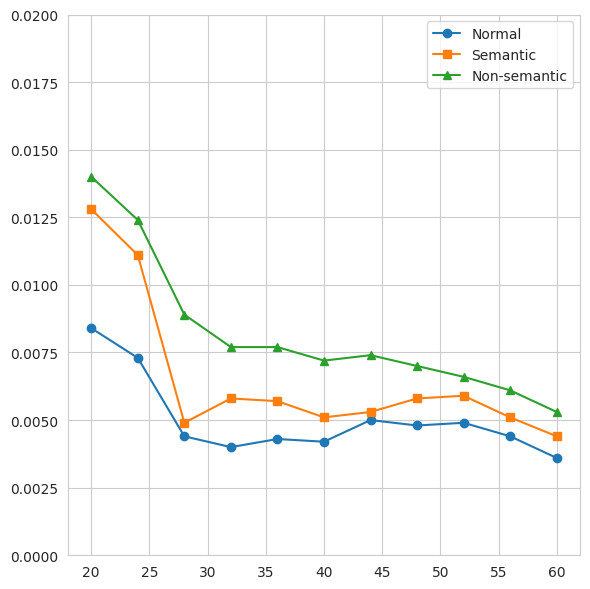
\includegraphics[width=\textwidth]{figures/rbad/assets/Synthesized Experiments/latest-eps=0.01, NNF-ratio=0.2, NRP-ratio=0.2, C-ratio=1.2, d-ratio=1.2.png}
       \caption{$c_3 = 1.2$}
       \label{fig-c_3=1.2}
   \end{subfigure}
   \hfill
   \begin{subfigure}[b]{0.3\textwidth}
       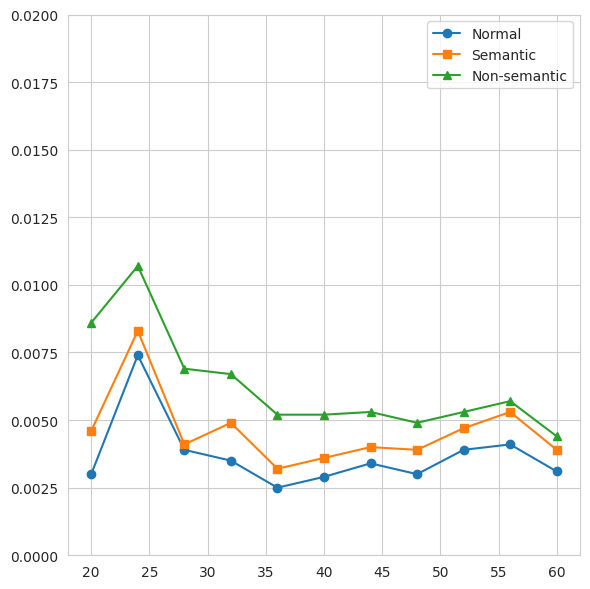
\includegraphics[width=\textwidth]{figures/rbad/assets/Synthesized Experiments/latest-eps=0.01, NNF-ratio=0.2, NRP-ratio=0.2, C-ratio=1.2, d-ratio=1.5.png}
       \caption{$c_3 = 1.5$}
       \label{fig-c_3=1.5}
   \end{subfigure}
   \hfill
   \begin{subfigure}[b]{0.3\textwidth}
       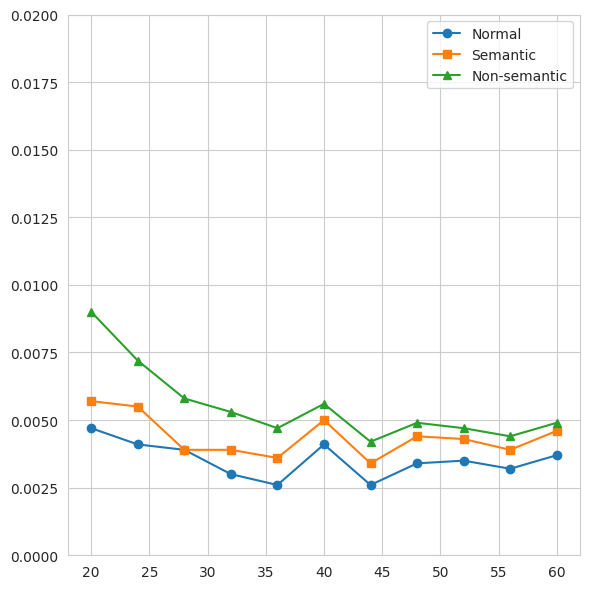
\includegraphics[width=\textwidth]{figures/rbad/assets/Synthesized Experiments/latest-eps=0.01, NNF-ratio=0.2, NRP-ratio=0.2, C-ratio=1.2, d-ratio=2.png}
       \caption{$c_3 = 2$}
       \label{fig-c_3=2}
   \end{subfigure}    
   \caption{\textbf{Results of the synthesized experiments}. 
   In these figures, the $x$-axis is the number of patches $P$. 
   The $y$-axis reports the reconstruction losses. 
   We let $d = {\rm{int}}(c_3 P)$ for $c_3 \in \{1.2, 1.5, 2\}$ and $C = {\rm{int}}(1.2 d)$ in the study.
   All of the experiments exhibit clear gaps between the reconstruction errors of the normal data and the non-semantic anomalies.
   Besides, as discussed in \ref{remark-semantic-anomalies-are-hard-to-detect}, the gap between the reconstruction errors of the normal data and the semantic anomalies is not as significant as that between the normal data and the non-semantic anomalies.}
\label{fig-synthesized-experiment-results}
\end{figure}

\paragraph{Visualization of the kernels}
   
\ref{fig-features-learned-by-autoencoder} visualize the first-layer features learned from MNIST and CIFAR-10, which validates our proposed cone set intuition.
It can be observed that the shapes and colors of the kernels do not significantly change during training because, as claimed in \ref{sec-main-results}, the kernels are absorbed by the cones of the features.
Notice that some of the kernels remain noisy even after 50 epochs.
We interpret these kernels as those $\w_j$ such that $j \notin \cup_{k\in [d]} \smost(k)$.
% The details of the experiments are reported in Appendix \ref{appendix-feature-visualization}.

\begin{figure}[H]
   \begin{center}
   
   \begin{subfigure}[b]{0.32\textwidth}
      \centering
      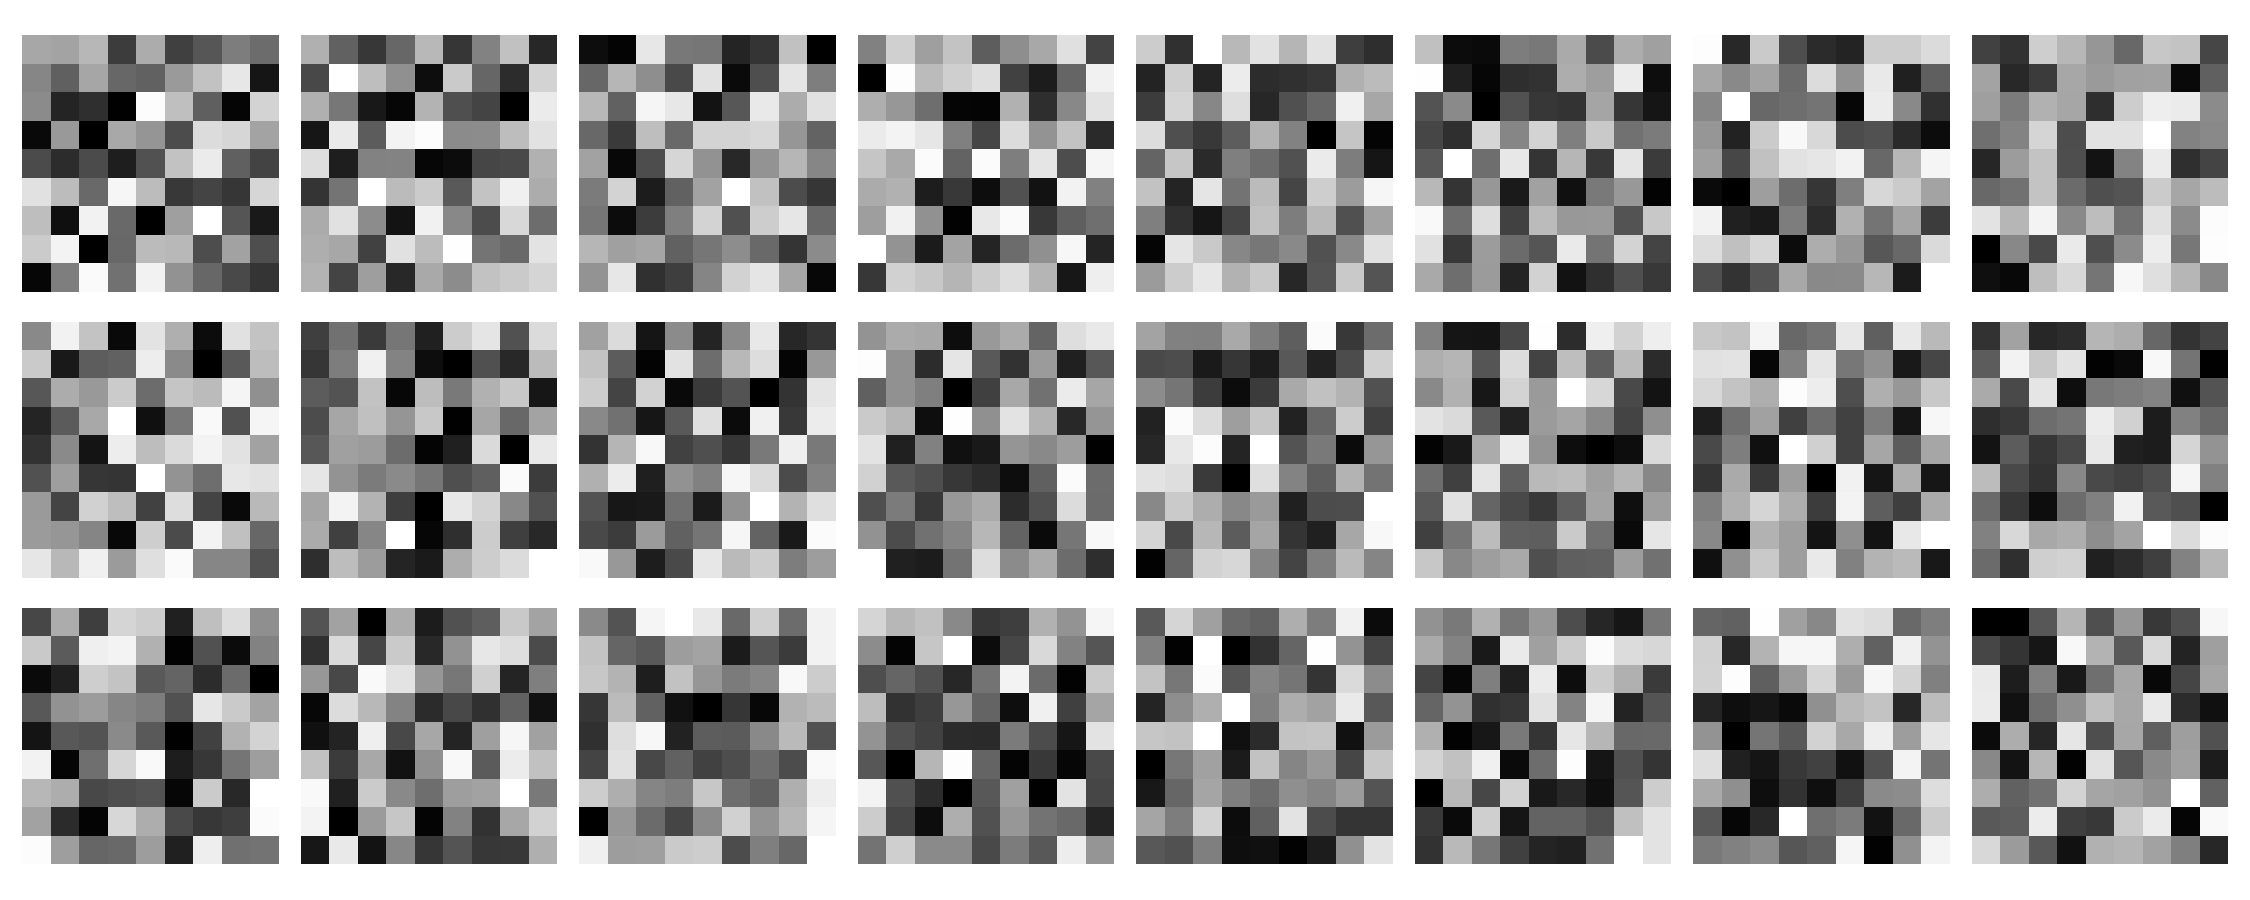
\includegraphics[width=\textwidth]{figures/rbad/assets/visualization/mnist_vae_0.pdf}
      \caption{Mnist, Epoch 0}
   \end{subfigure}
   \hfill
   \begin{subfigure}[b]{0.32\textwidth}
      \centering
      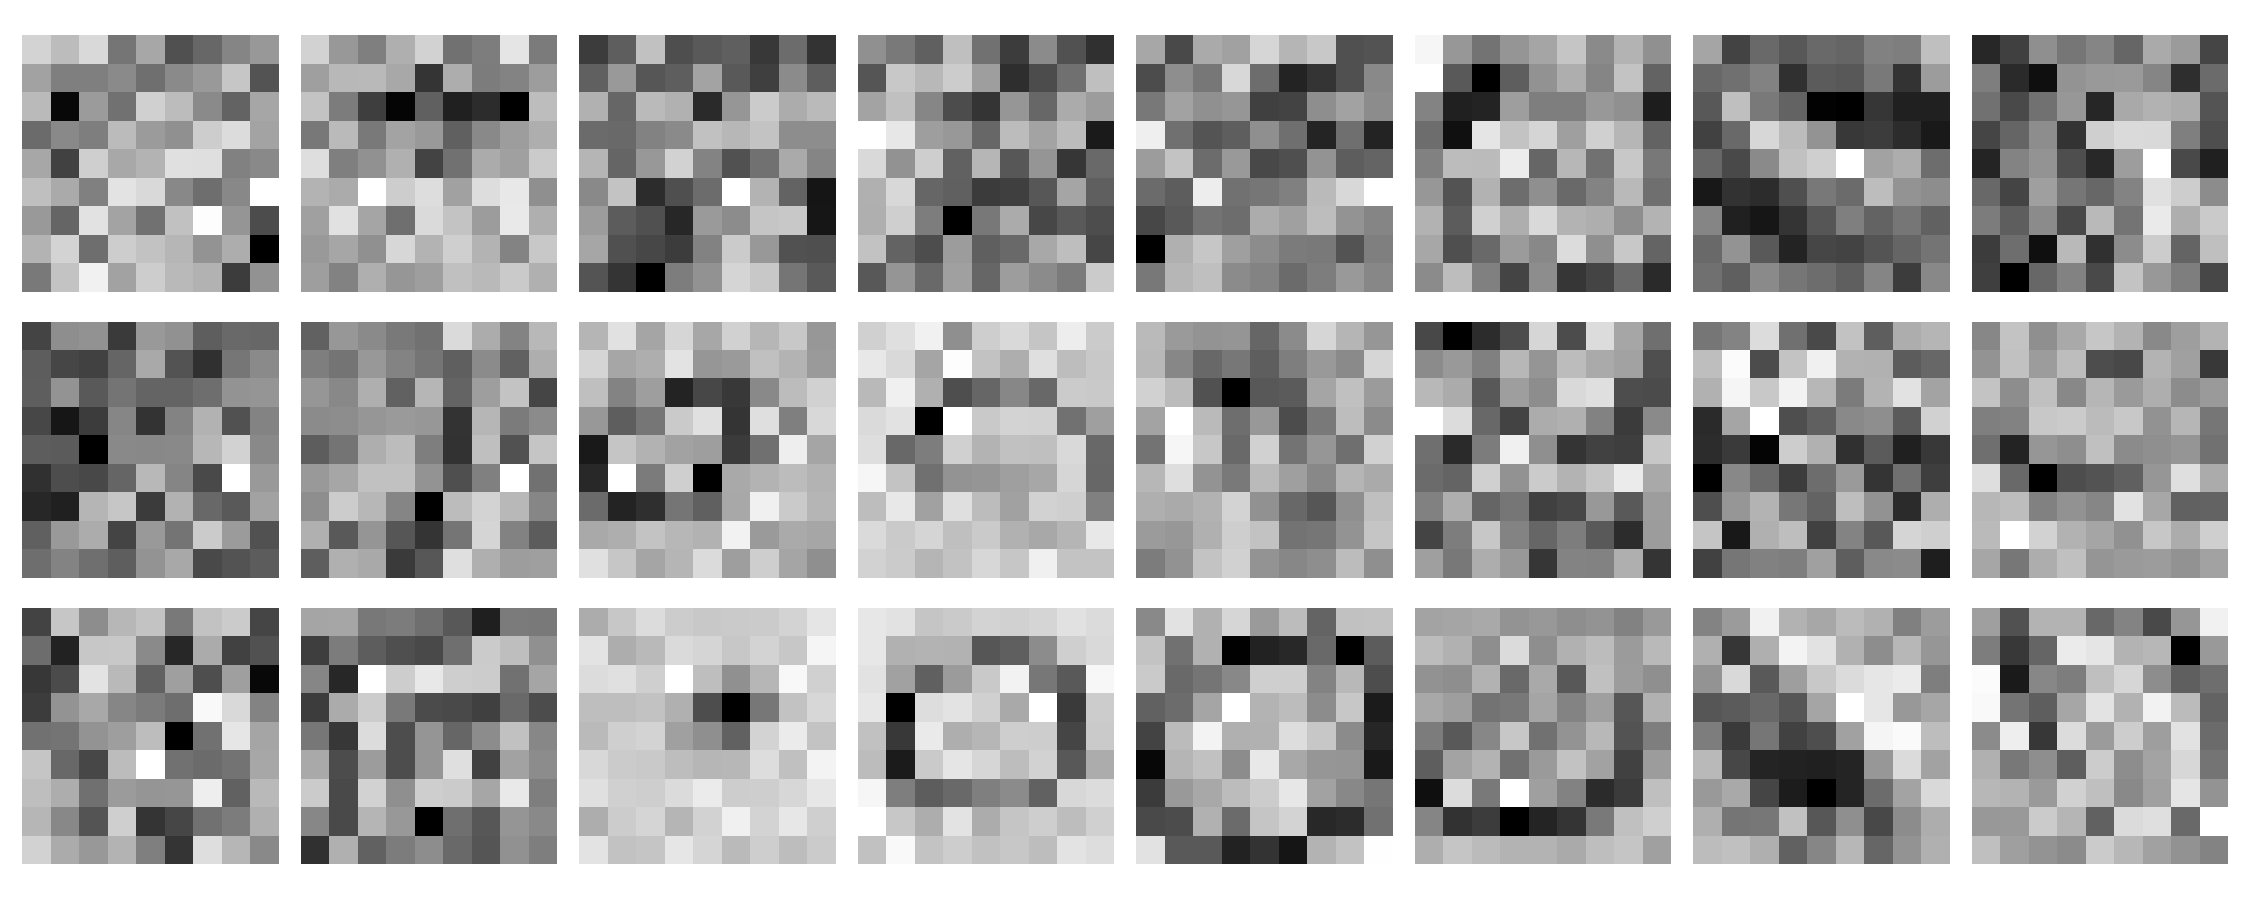
\includegraphics[width=\textwidth]{figures/rbad/assets/visualization/mnist_vae_10.pdf}
      \caption{Mnist, Epoch 10}
   \end{subfigure}
   \hfill
   \begin{subfigure}[b]{0.32\textwidth}
      \centering
      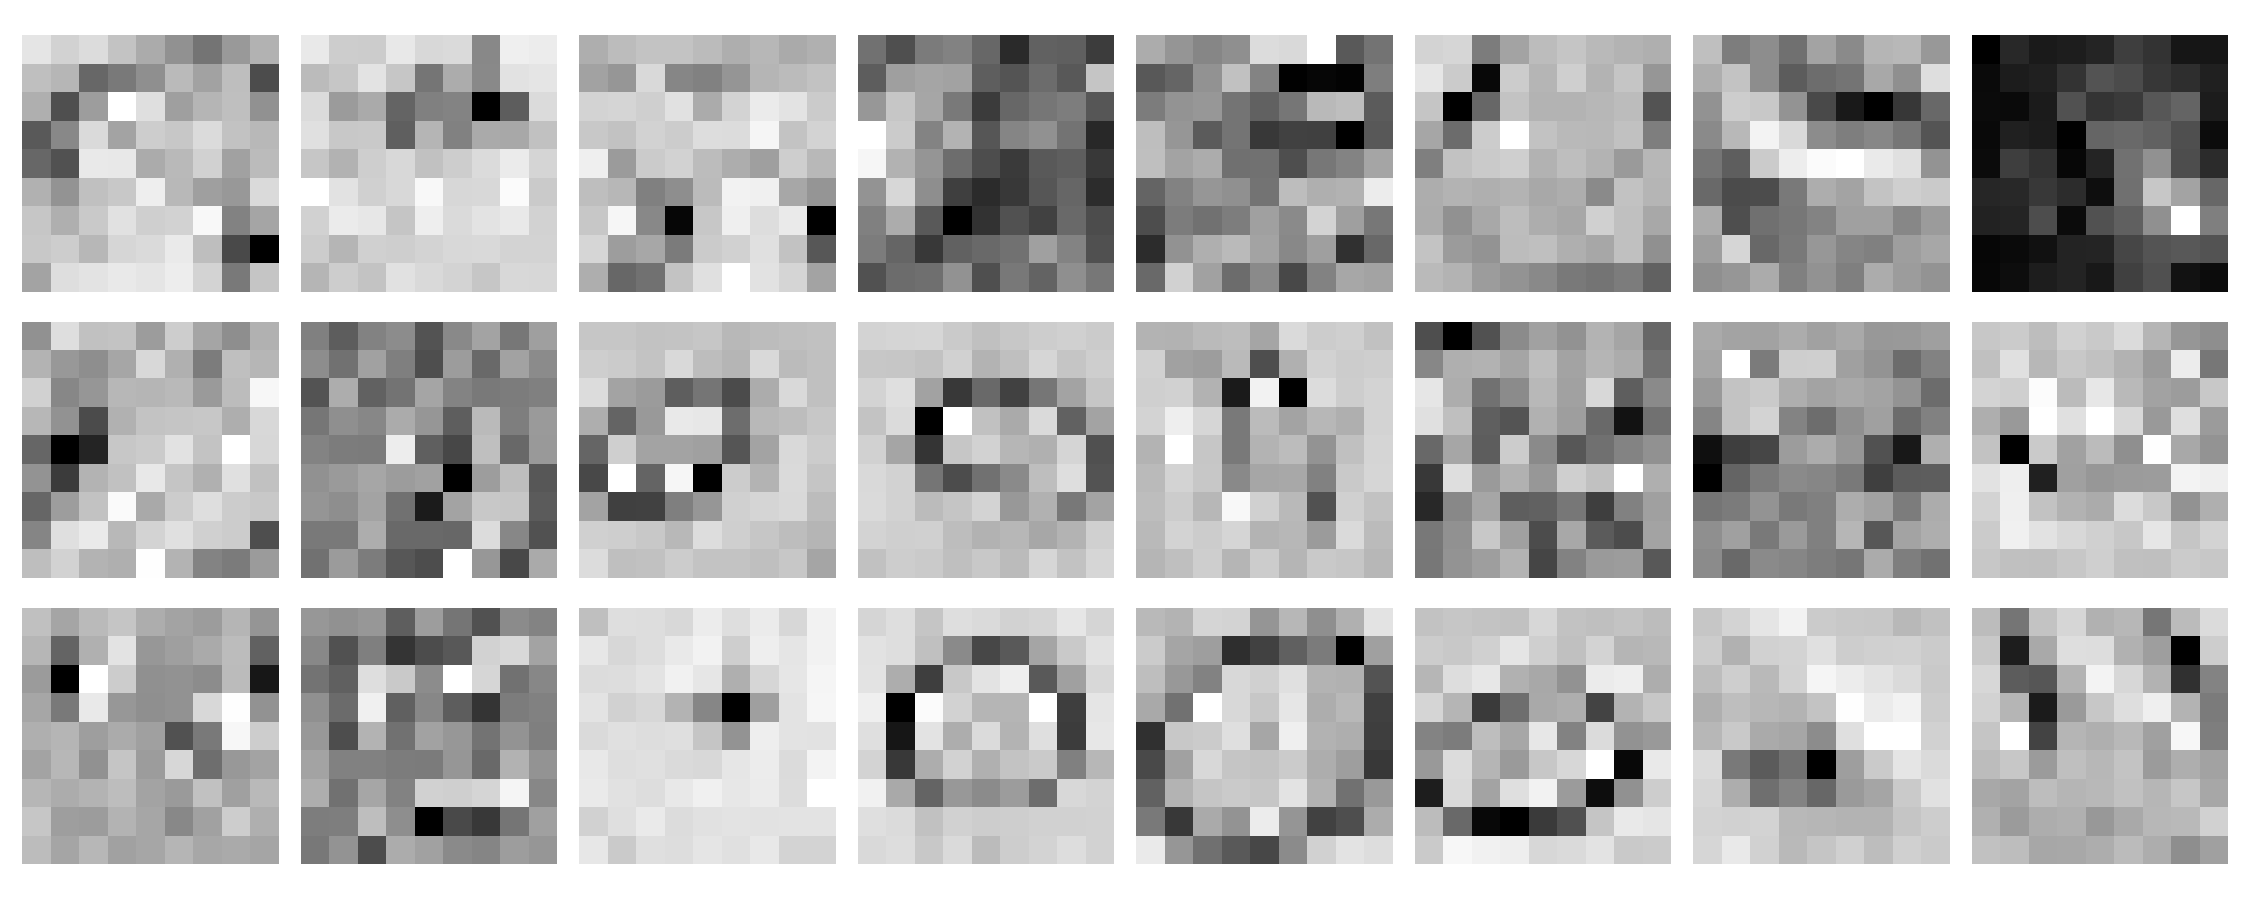
\includegraphics[width=\textwidth]{figures/rbad/assets/visualization/mnist_vae_50.pdf}
      \caption{Mnist, Epoch 50}
   \end{subfigure}
   
   \begin{subfigure}[b]{0.32\textwidth}
   \centering
   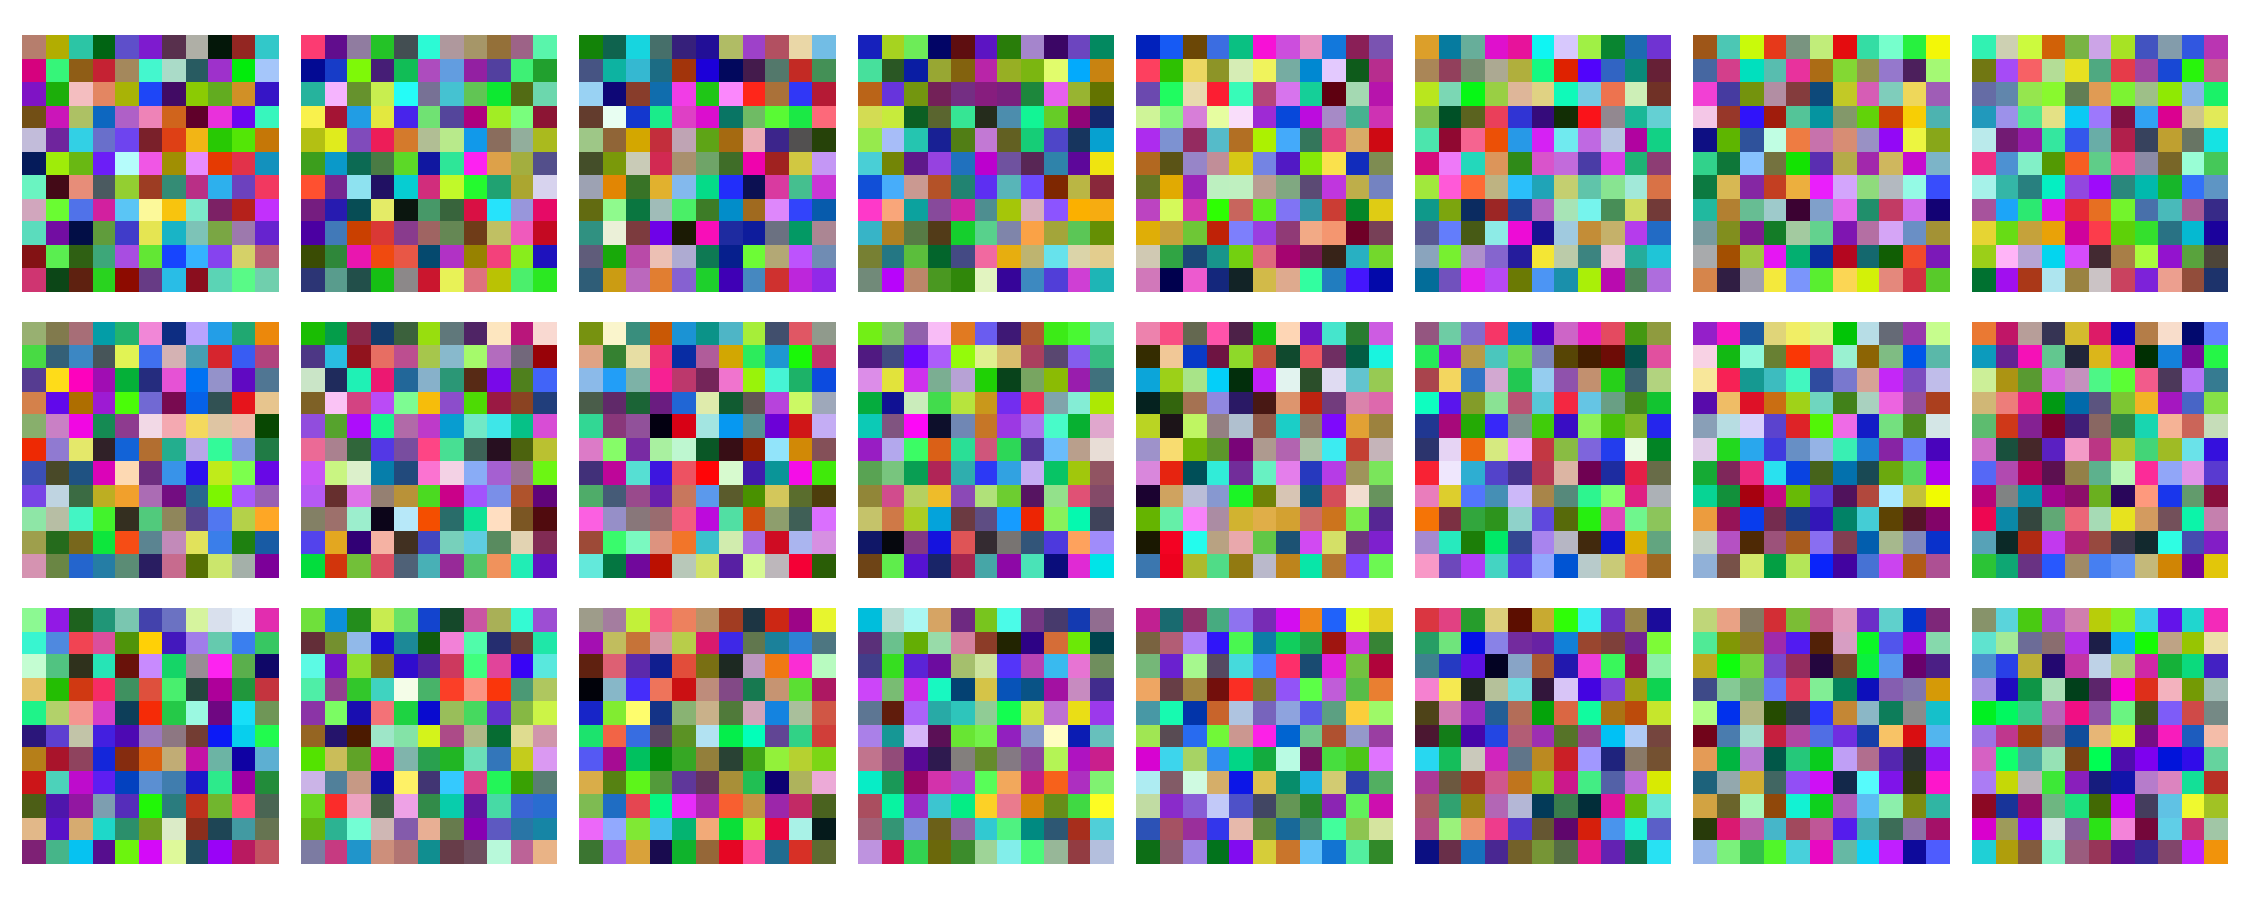
\includegraphics[width=\textwidth]{figures/rbad/assets/visualization/imagenet_scnn_0.pdf}
   \caption{CIFAR-10, Epoch 0}
   \end{subfigure}
   \hfill
   \begin{subfigure}[b]{0.32\textwidth}
   \centering
   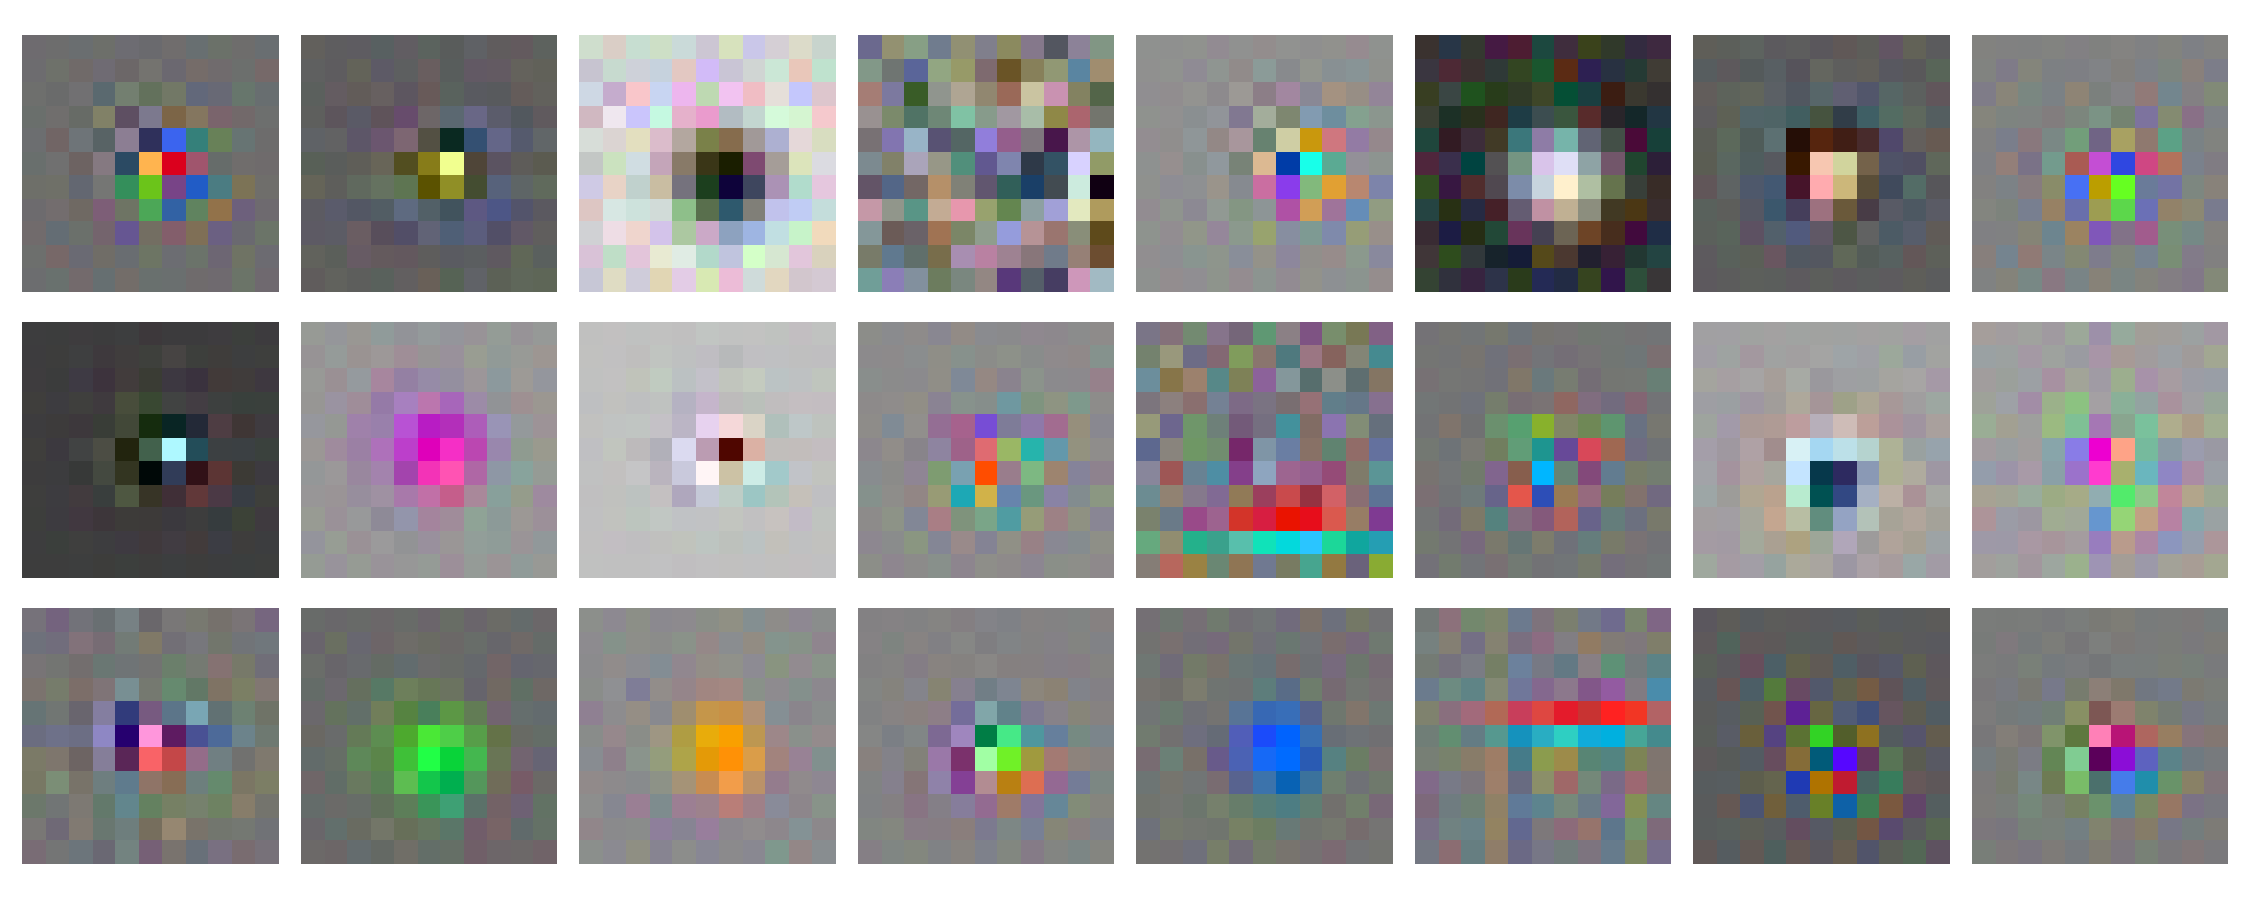
\includegraphics[width=\textwidth]{figures/rbad/assets/visualization/imagenet_scnn_10.pdf}
   \caption{CIFAR-10, Epoch 10}
   \end{subfigure}
   \hfill
   \begin{subfigure}[b]{0.32\textwidth}
   \centering
   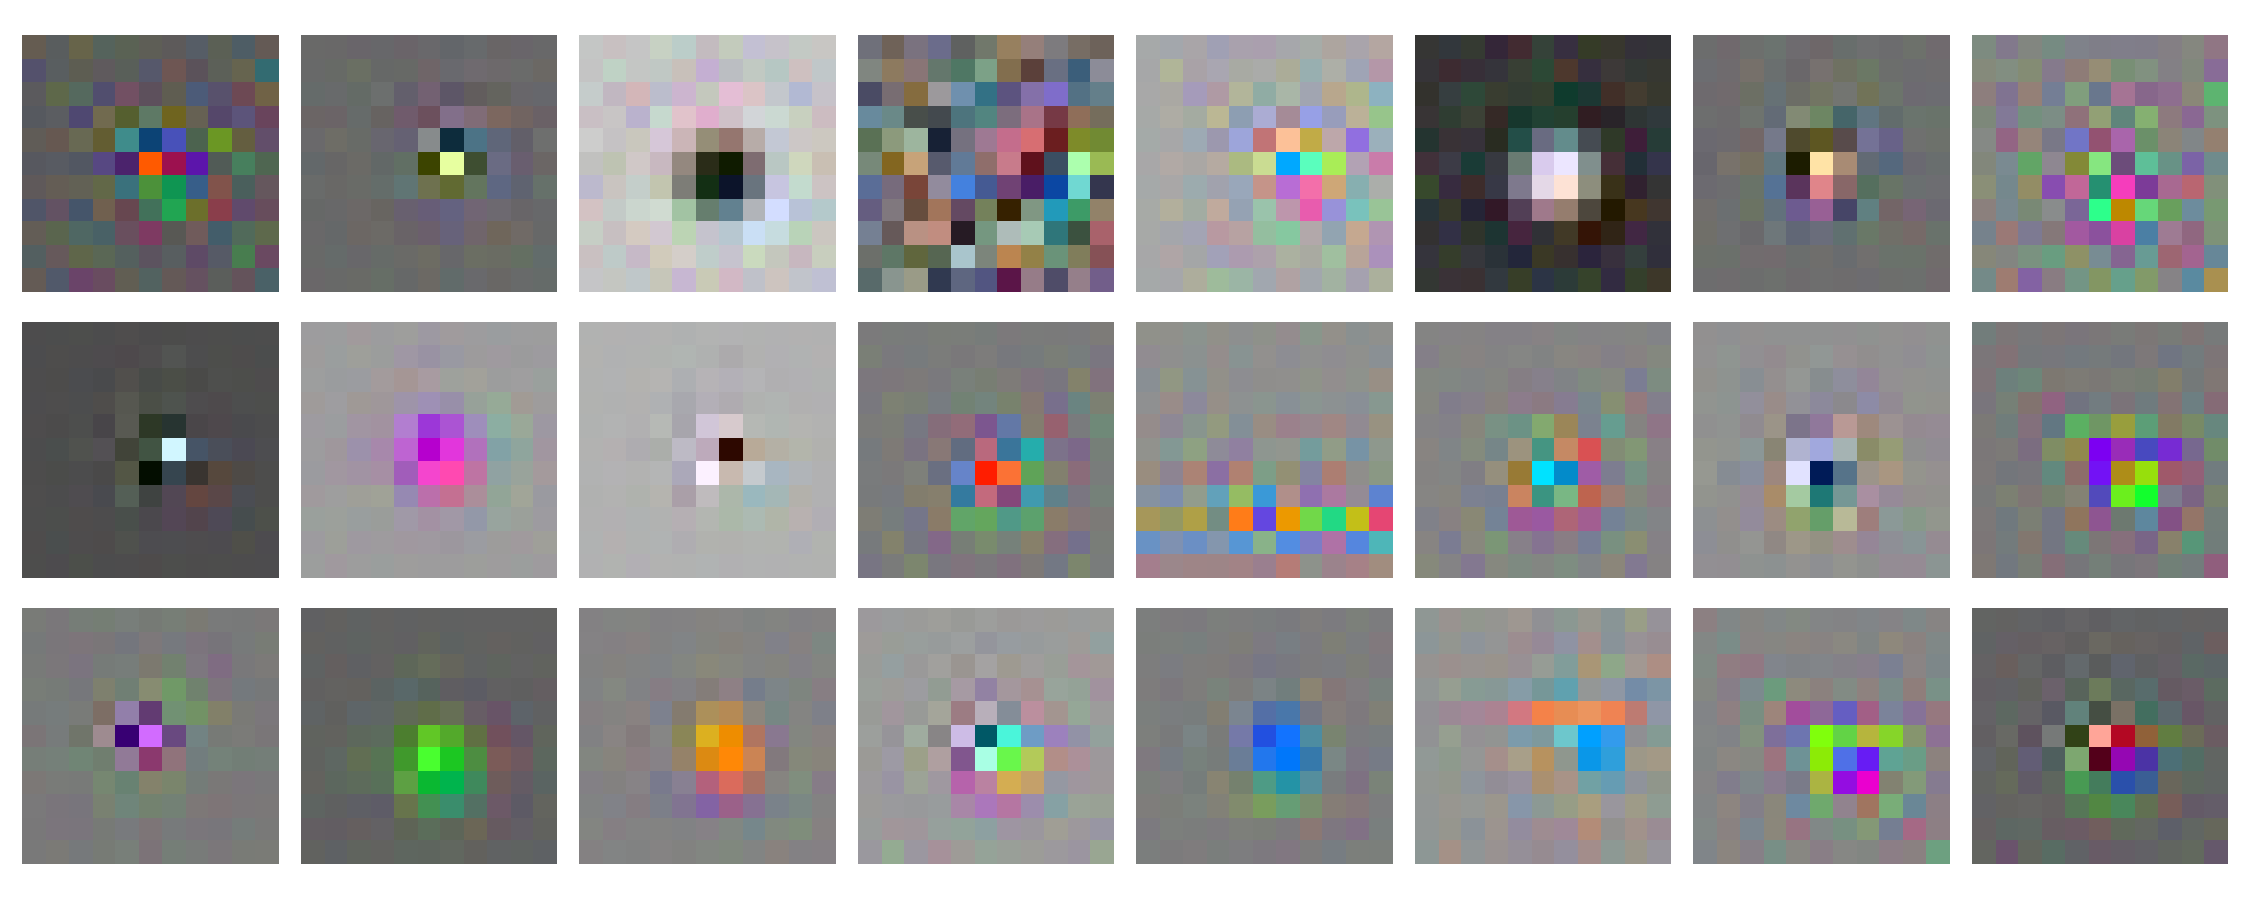
\includegraphics[width=\textwidth]{figures/rbad/assets/visualization/imagenet_scnn_40.pdf}
   \caption{CIFAR-10, Epoch 50}
   \end{subfigure}
   \end{center}
   \caption{Visualization of the kernels in the first layer of the autoencoder. }
   \label{fig-features-learned-by-autoencoder}
   \end{figure}

%%%%%%%%%%%%%%%%%%%%%%%%%%%%%%%%%%%%%%%%%%%%%%%%%%%%%%%%%%%%%%%%%%%%%%%
% Conclusion
%%%%%%%%%%%%%%%%%%%%%%%%%%%%%%%%%%%%%%%%%%%%%%%%%%%%%%%%%%%%%%%%%%%%%%%

\section{Conclusion}\label{sec-conclusion}
This paper studies the training dynamics of a 2-layer convolutional autoencoder and how it reconstructs different types of inputs. 
Particularly, we answer $\bm{Q}_1$ - $\bm{Q}_3$ raised in \ref{sec-introduction} as follows.

($\bm{Q}_1$) How does the model learn the features from training data in RBAD? 
($\bm{A}_1$) \textit{The kernels absorbed by the cone sets of the features would approximate the features.}

($\bm{Q}_2$) What is the role of the learned features in the reconstruction phase? 
($\bm{A}_2$) \textit{The features process the signal from the input patches and use them for reconstruction.}
    
($\bm{Q}_3$) Why are the anomalies harder to reconstruct? 
($\bm{A}_3$) \textit{The processed signal from the auxiliary features and the random noise is smaller than that from the normal features.}

Our theoretical findings and intuitions are supported by synthesized and real-world experiments.

\section{Complete Proofs}\label{sec-proof}
In this section, we go through the proofs in our analysis.
We use a separate numbering for the equations in this section so that the readers do not need to turn back to the main parts to reference the equations. 
Denote 
\begin{equation}
\Delta_{n,i} = \x_{n,i} - \phi_d^{(i)} (\phi_e(\z_n)),    
\end{equation}
i.e., the difference between the original patch $\x_{n,i}$ and the reconstructed patch $\phi_d^{(i)} (\phi_e(\z_n))$.
Then, the empirical reconstruction error can be written as
\begin{equation}
    \risk_N(\w) 
    = \frac{1}{N} \sum_{n \in [N]} \ell(\z_n;\w) 
    = \frac{1}{N} \sum_{n \in [N]} \| \phi(\z_n;\w) - \z_n \|^2 
    = \frac{1}{N} \sum_{n \in [N]} \sum_{i \in [P]} \ip{\Delta_{n,i},\Delta_{n,i}}.
\end{equation}
As a warm-up, the following proposition computes the gradient of $\risk_N(\w)$.
\begin{customprop}{\ref{prop-gradient}}
For all $ j \in [C]$, the gradient of the empirical reconstruction error is
\begin{equation}\label{eq-prop-gradient-gradient-in-proof}
\nabla_{\w_j} \risk_N(\w) = - \frac{2}{N} \!  \sum_{n,i} \delta_n(i,j) \left[ \sigma\! \left(\ip{\w_j,\x_{n,i}} \right) \Delta_{n,i} 
+  \ip{\Delta_{n,i}, \w_j} \sigma^{\prime}\!\left(\ip{\w_j,\x_{n,i}} \right) \x_{n,i} \right].
\end{equation}
\end{customprop}
\begin{proof}[Proof of Proposition \ref{prop-gradient}]
By definition, we have
\begin{equation} \label{eq-prop-gradient-nabla-R-N}
    \nabla_{\w_j} \risk_N(\w) 
    = \nabla_{\w_j} \left( \frac{1}{N} \sum_{n \in N} \ell(\z_n) \right) 
    = \frac{1}{N} \sum_{n \in [N]} \nabla_{\w_j} \ell(\z_n).
\end{equation}
Recall
\begin{equation}\label{eq-def-phi-d-in-proof}
\phi(\z;\w) = \phi_d \left(\phi_e(\z;\w) \right)
= \left( \phi_d^{(1)} \left(\phi_e(\z;\w) \right) , \cdots , \phi_d^{(P)}\left(\phi_e(\z;\w) \right) \right)
\end{equation}
and 
\begin{equation}\label{eq-def-loss-in-proof}
    \ell(\z;\w) = \| \phi(\z;\w) - \z \|^2.
\end{equation}
According to \ref{eq-def-phi-d-in-proof,eq-def-loss-in-proof}, for all $ n \in [N]$, we have
\begin{equation}
    \ell(\z_n) 
    = \| \phi(\z_n) - \z_n \|^2 
    = \sum_{i \in P}   \ip{ \phi_d^{(i)}(\phi_e(\z_n)) -\x_{n,i}, \phi_d^{(i)}(\phi_e(\z_n)) -\x_{n,i}} = \sum_{i \in [P]} \ip{\Delta_{n,i},\Delta_{n,i}},
\end{equation}
and the gradient of $\l(\z_n)$ can be written as
\begin{equation} \label{eq-prop-gradient-gradient-of-l-zn}
    \nabla_{\w_j} \left( \sum_{i \in P} \ip{\Delta_{n,i},\Delta_{n,i}} \right) 
    = \sum_{i \in P} 2 \left\langle \nabla_{\w_j}\Delta_{n,i}, \Delta_{n,i} \right\rangle
\end{equation}
Here, we abuse the notion of inner product $\ip{\nabla_{\w_j}\Delta_{n,i}, \Delta_{n,i}}$ to simplify the calculation of the gradient of $\l$ without causing confusion.  
Consider the right-hand side (RHS) of \ref{eq-prop-gradient-gradient-of-l-zn}.
For all $ i \in [P]$, the term in the sum equal to
\begin{equation}\label{eq-prop-gradient-2nabla-delta}
\begin{aligned}
    \left\langle \nabla_{\w_j}\Delta_{n,i}, \Delta_{n,i} \right\rangle
    &= \ip{\Delta_{n,i} , \nabla_{\w_j} \left( \x_{n,i} -  \sum_{{j^{\prime}} \in C} \sigma(\ip{\w_{j^{\prime}},\x_{n,i}}) \delta_n(i,{j^{\prime}}) \w_{j^{\prime}} \right) } \\
    &= - \ip{\Delta_{n,i} , \nabla_{\w_j} \left( \sum_{{j^{\prime}} \in \S_{n}(i)} \sigma(\ip{\w_{j^{\prime}},\x_{n,i}}) \w_{j^{\prime}} \right) }.
\end{aligned}
\end{equation}    
Here, $\delta_n(i,j)$ is the natural extension of $\delta(i,j)$, considering that $\x_i$ is replaced by $\x_{n,i}$ in the proof.
$\S_n(i)$ is defined as
\begin{equation}\label{eq-prop-gradient-def-Sni}
    \S_n(i) := \{ j \in [C] : \delta_n(i,{j{}}) = 1 \}.
\end{equation}
$\S_n(i)$ can be interpreted as the ``empirical cone set of the patch $\x_i$''.
From \ref{eq-prop-gradient-2nabla-delta} we know that $\left\langle \nabla_{\w_j}\Delta_{n,i}, \Delta_{n,i} \right\rangle$ takes $0$ when $j \notin \S_{n}(i)$.
Otherwise, we have
\begin{equation}
\begin{aligned}
   - \left\langle \nabla_{\w_j}\Delta_{n,i}, \Delta_{n,i} \right\rangle 
    &= \ip{\Delta_{n,i} , \nabla_{\w_j} \left( \sigma(\ip{\w_j,\x_{n,i}}) \w_j \right) }\\
    &= \sigma\left(\ip{\w_j,\x_{n,i}} \right)\Delta_{n,i} + \ip{\Delta_{n,i}, \w_j} \sigma^{\prime}\left(\ip{\w_j,\x_{n,i}}  \right) \x_{n,i},
\end{aligned}
\end{equation}
in which for all $ u \in \R$, the derivative of $\sigma$ at $u$ is 
\begin{equation}\label{eq-prop-gradient-sigma-prime}
    \sigma^{\prime}(u) = \left\{
    \begin{array}{cl}
        0 & \mbox{if } u \leq 0; \\
        (c_0)^{-1} x&\mbox{if }  0 < u \leq c_0; \\
        1& \mbox{if } u > c_0.
    \end{array}
    \right. 
\end{equation}
Finally, we can obtain \ref{eq-prop-gradient-gradient-in-proof} by combining Equations (\ref{eq-prop-gradient-nabla-R-N}) to (\ref{eq-prop-gradient-sigma-prime}), which completes the proof.
\end{proof}

% According to \ref{eq-prop-gradient-gradient}, for all $ j \in \S_{n,i}$, the gradient direction is composed of two major directions.
% Denote
% \begin{align}
%     \u_1(\w_j) &= \sum_{n \in N} \delta_n(i,j)  \sigma\left(\ip{\w_j,\x_{n,i}}   \right)\Delta_{n,i}, \label{eq-gradient-direction-1}\\ 
%     \u_2(\w_j) &= \sum_{n \in N} \delta_n(i,j) \ip{\Delta_{n,i}, \w_j} \sigma^{\prime}\left(\ip{\w_j,\x_{n,i}}  \right) \x_{n,i}, \label{eq-gradient-direction-2}
% \end{align}
% Intuitively, $\u_2$ should be closed $\x_{n,i}$ 
% \begin{align}
%     \u_{\x}(\w_j) &= \ip{\u_1(\w_j), \u_2(\w_j)} \u_2(\w_j) \\
%     \u_{\perp}(\w_j) &= \u_1(\w_j) - \ip{\u_1(\w_j), \u_2(\w_j)} \u_2(\w_j)
% \end{align}
% $\u_1$ and $\u_2$ are linearly independent in general.
% Otherwise, 

After random initialization, the kernels iterate according to the gradient descent rule, i.e.,  
\begin{equation}
    \w^{t+1}_j = \w^t_j - \eta_t \nabla_{\w_j} \risk_N(\w^t).
\end{equation} 
Let $f_h = f_h(d)$ be the control function of the growth of the major part of the kernels (i.e., the height of the cone in our cone set intuition.
At each iteration step, the size of the kernels can be bounded by the following lemma.

\begin{customlemma}{\ref{lemma-size-of-wj-in-paper}}
With probability at least $1 - p_0$, the random initialization of $\w_j^0$ satisfies
\begin{equation}\label{eq-lemma-size-of-wj-random-initialization}
    \|\w_j^0\| \leq \sigma_0 f_h.
\end{equation}
    For all $ t \geq 1$, the size of $\w_j^t$ is controlled by 
    \begin{equation}\label{eq-lemma-size-of-wj-result-2}
        \|\w_j^t\| \leq  t \sigma_0 f_h.
    \end{equation}
    with probability at least $1 - p_0$.
    In both \ref{eq-lemma-size-of-wj-random-initialization,eq-lemma-size-of-wj-result-2}, we let $p_0$ take
    \begin{equation}\label{eq-lemma-size-of-wj-p0}
         p_0 = 2\exp \left(- \frac{(f_h - d)^2}{8d}\right).
    \end{equation}
    % In particular, $f_h > d$
\end{customlemma}

\begin{proof}[Proof of Lemma \ref{lemma-size-of-wj-in-paper}]
    By definition, we can write
    \begin{equation}
        \w_j^0 = \left(  \w_j^{0,(1)}, \w_j^{0,(2)}, \cdots, \w_j^{0,(d)} \right)^T \sim \N(0,\sigma_0 \I)
    \end{equation}
    and
    \begin{equation}
        \frac{1}{\sigma_0^2}\|\w_j^0\|^2 = \sum_{i \in [d]} \left( \frac{\w_j^{0,(i)}}{\sigma_0} \right)^2 \sim \chi_d^2,
    \end{equation}
    in which $\chi_d^2$ is the chi-squared distribution with $d$ degrees of freedom.
    Lemma \ref{lemma-chi-square-concentration-inequality} implies that
    \begin{equation}\label{eq-lemma-size-of-wj-main-equation-1}
                \P \left[ \left| \|\w_j^0\|^2 - \sigma_0^2d \right| \geq \lambda \sigma_0^2 d \right] \leq 2 e^{-\lambda^2 d/8}
    \end{equation}
    for all $ \lambda \in (0,1)$.
    We can obtain \ref{eq-lemma-size-of-wj-random-initialization} by letting
    \begin{equation}
    \lambda = \frac{f_h^2 - d}{d}.    
    \end{equation}

    We prove the second result by induction. 
    \ref{eq-lemma-size-of-wj-main-equation-1} implies that $\|\w_j^{1}\| = \|\w_j^{0}\| \leq \sigma_0 f_h$ as required.
    For all $ t > 1$, assume that $\w_j^{t-1}$ satisfies \ref{eq-lemma-size-of-wj-result-2}.
    By definition, we have
    \begin{equation}\label{eq-lemma-size-of-wj-induction}
    \begin{aligned}
        &\|\w_j^{t}\| \\
        =& \left\| \w_j^{t-1} - \eta_{t-1} \nabla_{\w_j^{t-1}} \risk_N(\w^{t-1}) \right\| \\
        =& \left\|\w_j + \frac{\eta}{N} \! \! \!\sum_{n \in [N]} \sum_{i \in [P]} 2 \delta_n(i,j) \left[ \sigma\left(\ip{\w_j,\x_{n,i}}   \right) \Delta_{n,i} 
        + \ip{\Delta_{n,i}, \w_j} \sigma^{\prime}\left(\ip{\w_j,\x_{n,i}}  \right) \x_{n,i} \right] \right\| \\
        \leq& \|\w_j\| \! + \! \left\| \frac{\eta}{N}\! \! \! \sum_{n \in [N]} \sum_{i \in [P]} 2 \delta_n(i,j) \left[ \sigma\left(\ip{\w_j,\x_{n,i}}   \right) \Delta_{n,i} 
        \!+\! \ip{\Delta_{n,i}, \w_j} \sigma^{\prime}\left(\ip{\w_j,\x_{n,i}}  \right) \x_{n,i} \right] \right\|.
    \end{aligned}
    \end{equation}
    Due to limited space, the subscript or superscript of $t-1$ is omitted without causing any confusion. For all $ n \in [N]$ and $\forall i \in [P]$, it is easy to obtain that
    \begin{equation}
    \begin{aligned}
    &\| \sigma\left(\ip{\w_j,\x_{n,i}}   \right) \Delta_{n,i} 
    + \ip{\Delta_{n,i}, \w_j} \sigma^{\prime}\left(\ip{\w_j,\x_{n,i}}  \right) \x_{n,i} \| \\
    \leq &
    2 \|\x_{n,i}\| \|\Delta_{n,i}\| \|\w_j\| \\
    \leq  &
    2 (1+\epsilon)^2 \| \w_j \|.
    \end{aligned}
    \end{equation}
    Since only one of the $i \in [P]$ is counted in the second summation in \ref{eq-lemma-size-of-wj-induction} for all $ n \in [N]$ due to the property of $\delta_n(i,j)$, we have
    \begin{equation*}
    % \label{eq-lemma-size-of-wj-induction-result}
\left\| \frac{\eta}{N} \!\!\! \sum_{n \in [N]}\! \sum_{i \in [P]}\! 2 \delta_n(i,j)\! \left[ \sigma \! \left(\ip{\w_j,\x_{n,i}}   \right)\! \Delta_{n,i} 
       \! + \!\ip{\Delta_{n,i}, \w_j} \sigma^{\prime}\!\left(\ip{\w_j,\x_{n,i}}  \right) \x_{n,i} \right] \right\|
        \!\leq \! 4 (1+\epsilon)^2 \eta \| \w_j \|,
    \end{equation*}
    which implies that
    \begin{equation}\label{eq-lemma-size-of-wj-induction-final-result}
        \|\w_j^{t}\| \leq (1 + 5 \eta_{t-1})\|\w_j^{t-1}\|.
    \end{equation}
    We can obtain \ref{eq-lemma-size-of-wj-result-2} by taking $\eta_t = 0.2t^{-1}$ into \ref{eq-lemma-size-of-wj-induction-final-result}, which finishes the proof of this lemma.
\end{proof}

\begin{customlemma}{\ref{lemma-smost-delta-ij-in-paper}}
    For all $ t \geq 1$, if $j \in \smost^t(k)$ and $\x_i$ (or $\x_{n,i}$) contains $\v_k$, then we 
 have $\delta(i,j) = 1$ (or $\delta_n(i,j) = 1$).
\end{customlemma}
\begin{proof}\label{proof-lemma-smost-delta-ij}
    Recall that $\delta(i,j)$ is a binary-value function that takes $1$ when 
    \begin{equation}
            i = \argmax_{i^{\prime} \in [P]} \sigma(\ip{\w^t_j,\x_{i^{\prime}}})
    \end{equation}
and $0$ otherwise.
    Since $\sigma$ is non-decreasing, we have
    \begin{equation}
        \argmax_{i \in [P]} \sigma(\ip{\w_j,\x_i}) = \argmax_{i \in [P]} \ip{\w_j,\x_i}.
    \end{equation}
When $j \in \smost^t(k)$ and $\x_i$ contains $\v_k$, $\ip{ \w_j , \x_{i} }$ can be bounded by
    \begin{equation}\label{eq-lemma-smost-delta-ij-upper}\begin{aligned}
        \ip{ \w_j^t , \x_{i} } 
        &= \ip{ \w_j^t , \v_{k} } + \ip{ \w_j^t , \x_{i} - \v_{k} } \\
        &\geq  t \sigma_0 c_1 f_h - \|\w_j^t\| \| \x_i - \v_k \| \\
        &\geq (c_1 - \sqrt{2\epsilon}) t \sigma_0 f_h.
    \end{aligned}\end{equation}
On the other hand, consider $i^{\prime}$ and $k^{\prime}$ such that $\x_{i^{\prime}}$ contains $\v_{k^{\prime}}$.
    By Assumption \ref{assumption-normal-data}, $k^{\prime} \neq k$ if given $i^{\prime} \neq i$.
    Therefore, we have
    \begin{equation}\label{eq-lemma-smost-delta-ij-lower}\begin{aligned}
        \ip{ \w_j , \x_{i^{\prime}} } 
        &= \ip{ \w_j , \v_{k^{\prime} } } + \ip{ \w_j , \x_{i^{\prime} } - \v_{k^{\prime} } } \\
        &\leq t \sigma_0 f_r + \|\w_j\| \| \x_i - \v_k \| \\
        &\leq (f_r +  \sqrt{2\epsilon} f_h ) t \sigma_0 
    \end{aligned}\end{equation}
    We prove the lemma by combining \ref{eq-lemma-smost-delta-ij-upper,eq-lemma-smost-delta-ij-lower}.
\end{proof}

% \begin{remark}[Relationship between $\smost^t(k)$ and $\S_n^t(i)$]
%     This paper uses $\smost^t(k)$ and $\S_n^t(i)$ (defined in \ref{eq-prop-gradient-def-Sni}) to represent the collection index $j \in [C]$ such that $\w_j^t$ is \qm{highly related} to $\v_k$ and $\x_{n,i}$, respectively. 
%     Lemma \ref{lemma-smost-delta-ij} reveals the relationship between these two similar notations.
%     For all $ t \geq 1$, $\x_{n,i}$ contains $\v_k$ implies that $\smost^t(k) \subset \S_n^t(i)$, but the inverse is not true in general. \myqed 
% \end{remark}


Denote
\begin{equation}\label{eq-def-p1}
    p_1 =  
    \left( \frac{c_1 f_h}{(c_1 f_h)^2 + 1} \frac{ e^{-(c_1 f_h)^2} }{\sqrt{2\pi}} \right)
    \left(1 - \frac{1}{f_r} \frac{ e^{-f_r^2} }{\sqrt{2\pi}} \right)^{C-1}
\end{equation}
and
\begin{equation}\label{eq-def-p2}
    p_2 = 
    \left( \frac{1}{c_1f_h} \frac{ e^{-(c_1f_h)^2} }{\sqrt{2\pi}} \right)
    \left(1 - \frac{f_r}{f_r^2 + 1} \frac{ e^{-f_r^2} }{\sqrt{2\pi}} \right)^{C-1}.
\end{equation}
The following lemma proves that the size of $\smost$ at random initialization is bounded from both sides.
Note that $\w^0 = \w^1$ since we set $\eta_0 = 0$.
\begin{customlemma}{\ref{theorem-initial-size-in-paper}}
Let $p_1$ and $p_2$ be parameters depending on $d$ and $t$.
For all $ k \in [d]$, the size of $\smost^0(k)$ can be upper-bounded by
\begin{equation}
     | \smost^0(k) |  \leq C p_2 + \lambda,
\end{equation}
with probability at least $ 1 - \exp\left( - \frac{3\lambda^2}{6C p_2 + 2\lambda} \right)$ over random initialization.
The lower-bound
\begin{equation}
    | \smost^0(k) | \geq C p_1 - \lambda
\end{equation}
hold with probability at least $1 - \exp \left( - \frac{\lambda^2}{2 C p_2} \right)$.
\end{customlemma}
\begin{proof}[Proof of \ref{theorem-initial-size-in-paper}]
According to \cite{Dumbgen10}, we have 
\begin{equation}\label{eq-lemma-init-prob-smost-dumbgen10}
    \frac{1}{x + 1/x} \frac{ e^{-x^2} }{\sqrt{2\pi}}
     < \mathop{\P}_{g \sim \N(0,1)} \left[ g > x \right]
     < \frac{1}{x} \frac{ e^{-x^2} }{\sqrt{2\pi}}
\end{equation}
for arbitrary $x > 0$. 
For all $ j \in [C]$, we have
\begin{equation}\label{eq-lemma-inti-prob-constraint-1}
    \frac{\langle{\w_j^1, \v_k \rangle}}{\sigma_0} = \sum_{k \in [d]} \v_k^{(k)} \frac{\w_j^{1,(k)}}{\sigma_0}  \sim \N(0,1).
\end{equation}
Take $x = c_1 f_h $ in \ref{eq-lemma-init-prob-smost-dumbgen10}, we can obtain
\begin{equation}\label{eq-lemma-inti-prob-4-pm-c0}
\frac{c_1 f_h}{(c_1 f_h)^2 + 1} \frac{ e^{-(c_1 f_h)^2} }{\sqrt{2\pi}}
 < {\P}_{\w_j^{0}} \left[ \ip{\w_j^1, \v_k} > \sigma_0 c_1 f_h \right]
 < \frac{1}{c_1f_h} \frac{ e^{-(c_1f_h)^2} }{\sqrt{2\pi}}.
\end{equation}
Similarly, we have
\begin{equation}\label{eq-lemma-inti-prob-constraint-2}
\frac{f_r}{f_r^2 + 1} \frac{ e^{-f_r^2} }{\sqrt{2\pi}}
 < {\P}_{\w_j^{0}} \left[ \ip{\w_j^1, \v_k} > \sigma_0 f_r \right]
 < \frac{1}{f_r} \frac{ e^{-f_r^2} }{\sqrt{2\pi}}.
\end{equation}
by letting $x = f_r$.
By definition, we have
\begin{equation}\label{eq-lemma-inti-prob-by-def-smost}
    {\P}_{\w^{0}} \left[ j \in  \smost^0(k) \right] = 
    {\P}_{\w_j^{0}} \left[ \ip{\w_j^1, \v_k} > \sigma_0 c_1 f_h \right] \cdot 
    \left( 1 -  {\P}_{\w_j^{0}} \left[ \ip{\w_j^1, \v_k} > \sigma_0 f_r \right] \right)^{C-1}.
\end{equation}
Combining \ref{eq-lemma-inti-prob-4-pm-c0,eq-lemma-inti-prob-constraint-2,eq-lemma-inti-prob-by-def-smost}, we obtain that
\begin{equation}
    p_1 \leq {\P}_{\w_j^{0}} \left[ j \in  \smost^0(k) \right] \leq p_2
\end{equation}
By \ref{corollary-cp-lambda} we immediately get \ref{eq-lemma-init-prob-smost-result-upper-bound,eq-lemma-init-prob-smost-result-lower-bound}.
\end{proof}

% In the rest of this paper, we use the following slightly weaker result that can be viewed as a simple corollary of Lemma \ref{lemma-init-prob-smost}.
% \begin{corollary}\label{corollary-init-prob-smost}
    
% \end{corollary}


% In a similar sense, Definition \ref{def-sless,def-snot} introduces the collection of kernels that are \textit{less} or \textit{not} related to feature $i$.

% \begin{definition}[Less related kernels]\label{def-sless}
%     Let $\sless^t(k)$ be the collection of indices $j \in [C]$ such that
% \begin{itemize}
%     \item $ \ip{ \w_j^{t} , \v_{k} } \geq t \sigma_0 f_r $, and
%     \item for all $ k^{\prime} \neq k $, $ \ip{ \w_{j}^{t} ,  \v_{k^{\prime}} } \leq t \sigma_0 f_r $. \myqed
% \end{itemize}
% \end{definition}

% \begin{definition}[Not related kernels]\label{def-snot}
%     Let $\snot^t$ be the collection of indices $j \in [C]$ such that
%     \begin{equation}
%          \ip{ \w_j^{t} , \v_{k} } < t \sigma_0 f_r 
%     \end{equation}
%     for all $ k \in [d]$. \myqed
% \end{definition}

% Lemma \ref{lemma-init-prob-sless,lemma-init-prob-snot} bound the initial size of $\sless$ and $\snot$, respectively.
% \begin{lemma}[Size of $\sless$ at random initialization]\label{lemma-init-prob-sless}
% For all $ k \in [P]$, with probability at least $1 - $ over random initialization, the size of $\sless^0(k)$ can be controlled by
    
% \end{lemma}

% \begin{lemma}[Size of $\snot$ at random initialization]\label{lemma-init-prob-snot}
% For all $ i \in [P]$, with probability at least $1 - $ over random initialization, the size of $\snot^0$ can be controlled by
    
% \end{lemma}

% \begin{lemma}
% With probability at least $1 - p_4$
%     \begin{equation}
%         |\S| < \frac{c_2 C}{d}
%     \end{equation}
% \end{lemma}
% As discussed in \ref{sec-main-results}, the growth of kernels is determined after initialization. 

% \begin{remark}[Simplifying the max pooling operation]\label{remark-simplify-delta}
    
% \end{remark}

% \subsection{Main Results}
% \begin{itemize}
%     \item if $j \in \smost(k)$, (1) $\Delta \ip{\w_j,v_k} \geq \sigma_0 c_1 ((t+1)f_h(t+1,d) - t f_h(t,d))$ and (2) $\Delta \ip{\w_j,v_{k^{\prime}}} \leq \sigma_0 f_r$
%     \item if $j \in \sless(k)$, (1) $\Delta \ip{\w_j,v_k} \geq \sigma_0 c_1 f_h$ and (2) $\Delta \ip{\w_j,v_{k^{\prime}}} \leq \sigma_0 f_r$
% \end{itemize}

\begin{customthm}{\ref{theorem-Stk-subset-st+1k}}
    Assume that $|\smost^{0}(k)| \geq 1$ for all $k \in [d]$.
    For all $ t \in [T]$ and $\forall k \in [d]$, we have $\smost^{t}(k) \subseteq \smost^{t+1}(k)$.
\end{customthm}

\begin{proof}[Proof of \ref{theorem-Stk-subset-st+1k}]
% \begin{equation}
%     \w^{t+1}_j - \w^{t}_j = \sum_{i \in d} \ip{\w^{t+1}_j - \w^{t}_j,\v_k} \v_k
% \end{equation}
We prove $\smost^{t}(k) \subseteq \smost^{t+1}(k)$ by induction. 
For any $j \in [C]$, assume that $\w_j \in \smost^{t}(k)$ at iteration $t$. 
The growth of $\w_{j}^{t}$ along $\v_k$ is given by
\begin{equation}\label{eq-theorem-phase-I-main-wjt+1-wjt}
\begin{aligned}
    \ip{\w^{t+1}_j - \w^{t}_j,\v_k} 
    =& \ip{ - \eta_t \nabla_{\w_j^{t}} \risk_N (\w) , \v_k}  \\
    =& \sum_{n \in [N]} \sum_{i \in [P]} 2 \eta_t \delta_n(i,j) \left[ \sigma\left(\ip{\w_j^{t},\x_{n,i}}   \right) \ip{\Delta_{n,i},\v_k} 
    {+} \ip{\Delta_{n,i}, \w_j^{t}} \sigma^{\prime}\left(\ip{\w_j^{t},\x_{n,i}}  \right) \ip{\x_{n,i},\v_k} \right]
\end{aligned}
\end{equation}

Given $n \in [N]$, suppose $\exists \x_{n,i_n}$ such that $\x_{n,i_n}$ contains $\v_k$.
By definition, this condition holds for $\beta_k N$ many training samples.
Then, Lemma \ref{lemma-smost-delta-ij-in-paper} implies that
\begin{equation}\label{eq-theorem-phase-I-main-xni-contains-vk}
\begin{aligned}
    &\sum_{i \in [P]} \delta_n(i,j) \left[ \sigma\left(\ip{\w_j^{t},\x_{n,i}}   \right) \ip{\Delta_{n,i},\v_k} 
    {+} \ip{\Delta_{n,i}, \w_j^{t}} \sigma^{\prime}\left(\ip{\w_j^{t},\x_{n,i}}  \right) \ip{\x_{n,i},\v_k} \right] \\
    = \ & \sigma\left(\ip{\w_j^{t},\x_{n,i_n}}   \right) \ip{\Delta_{n,i_n},\v_k} 
    {+} \ip{\Delta_{n,i_n}, \w_j^{t}} \sigma^{\prime}\left(\ip{\w_j^{t},\x_{n,i_n}}  \right) \ip{\x_{n,i_n},\v_k}.
\end{aligned}
\end{equation}


Otherwise, given $n \in [N]$, we let $\x_{n,i_n} := 0$ when there is no $\x_{n,i}$ such that $\x_{n,i}$ contains $\v_k$ with slight abuse of notation.
Using these notations, we can write
\begin{equation}\label{eq-theorem-phase-I-main-smost-combine}
    \ip{\w^{t+1}_j - \w^{t}_j,\v_k}
    = 2 \eta_t \sum_{n \in [N]} \sigma\left(\ip{\w_j^{t},\x_{n,i_n}}   \right) \ip{\Delta_{n,i_n},\v_k} 
    {+} \ip{\Delta_{n,i_n}, \w_j^{t}} \sigma^{\prime}\left(\ip{\w_j^{t},\x_{n,i_n}}  \right) \ip{\x_{n,i_n},\v_k} 
\end{equation}

It remains to bound the terms in \ref{eq-theorem-phase-I-main-smost-combine}.
We first look at $\ip{\Delta_{n,i_n},\v_k} $.
\begin{equation}\label{eq-theorem-phase-I-main-sum-ip-delta-ni-vi}
\begin{aligned}
    \ip{\Delta_{n,i_n},\v_k} 
    &= \ip{ \left(\x_{n,i_n} - \sum_{{j^{\prime}} \in \S_{n}(i_n)} \relu{\ip{\w_{j^{\prime}}^{t},\x_{n,i_n}}  } \w_{j^{\prime}}^{t} \right), \v_k } \\
    &= \ip{ \x_{n,i_n}, \v_k } - \ip{ \sum_{{j^{\prime}} \in \S_{n}(i_n)} \relu{\ip{\w_{j^{\prime}}^{t},\x_{n,i_n}}  } \w_{j^{\prime}}^{t}, \v_k } \\
    &= \ip{ \x_{n,i_n}, \v_k } -  \sum_{{j^{\prime}} \in \S_{n}(i_n)} \ip{  \relu{\ip{\w_{j^{\prime}}^{t},\x_{n,i_n}}  } \w_{j^{\prime}}^{t}, \v_k }
\end{aligned}
\end{equation}
Apparently, both sides of \ref{eq-theorem-phase-I-main-sum-ip-delta-ni-vi} would take zero if $\x_{n,i_n} = 0$.
We only need to consider the case when $\x_{n,i_n} \neq 0$. 
Since $\x_{n,i_n}$ contains $\v_k$, for all $ j^{\prime} \in \S_{n}(i_n) $, we have 
\begin{equation}\label{eq-theorem-phase-I-main-sigma-wj-xni-leq-wjvi}
\begin{aligned}
    \relu{\ip{\w_{j^{\prime}}^{t},\x_{n,i_n}}  } &\leq \ip{\w_{j^{\prime}}^{t},\x_{n,i_n}}   \\
    &= \ip{\w_{j^{\prime}}^{t}, \v_k} + \ip{\w_{j^{\prime}}^{t},\x_{n,i_n} - \v_k }   \\
    &\leq \ip{\w_{j^{\prime}}^{t}, \v_k} + \sqrt{2\epsilon} \|\w_{j^{\prime}}^t\|   \\ % TODO: b限制条件
    % &\leq (1 + \sqrt{2\epsilon})\| \w_{j^{\prime}}^{t} \|.
    &\leq (1 + \sqrt{2\epsilon}) \wbound.
\end{aligned}
\end{equation}
Lemma \ref{lemma-smost-delta-ij-in-paper} implies that \ref{eq-theorem-phase-I-main-sigma-wj-xni-leq-wjvi} also hold for $\relu{\ip{\w_j^{t},\x_{n,i_n}}  }$ since $j \in \smost^t(k)$. 
Combining \ref{eq-theorem-phase-I-main-sum-ip-delta-ni-vi,eq-theorem-phase-I-main-sigma-wj-xni-leq-wjvi}, we have
\begin{equation}
    \ip{\Delta_{n,i},\v_k} 
    \geq 1 - \epsilon 
    - (1 + \sqrt{2\epsilon})\sum_{{j^{\prime}} \in \S_{n}(i_n)} \|\w_{j^{\prime}}^{t}\|^2
    \geq 1 - \epsilon - (1 + \sqrt{2 \epsilon})(\wbound)^2|\S^t_n(i_n)|.
\end{equation}
Since we assume $\smost^{0}(k) \geq 1$ for all features, we have
\begin{equation}
    |\S^t_n(i_n)| \leq (c_2 - 1) d.
\end{equation}
Next, we turn to $\ip{\Delta_{n,i},\w_j^{t}}$.
Similarly, we have
\begin{equation}\label{eq-theorem-phase-I-main-sum-deltani-vi}
\begin{aligned}
    \ip{\Delta_{n,i},\w_j^{t}} 
    &= \ip{ \left(\x_{n,i} - \sum_{j^{\prime} \in \S_{n,i}} \relu{\ip{\w_{j^{\prime}}^{t},\x_{n,i}}  } \w_{j^{\prime}}^{t} \right), \w_j^{t} } \\
    &= \ip{ \x_{n,i}, \w_j^{t} } - \ip{ \sum_{j^{\prime} \in \S_{n,i}} \relu{\ip{\w_{j^{\prime}}^{t},\x_{n,i}}  } \w_{j^{\prime}}^{t}, \w_j^{t} } \\
    &= \ip{ \x_{n,i}, \w_j^{t} } - \sum_{j^{\prime} \in \S_{n,i}} \ip{ \relu{\ip{\w_{j^{\prime}}^{t},\x_{n,i}}  } \w_{j^{\prime}}^{t}, \w_j^{t} } \\
    &\geq \ip{\w_j^{t}, \v_k} - \sqrt{2\epsilon} \|\w_j^t\| - (1 + \sqrt{2\epsilon})\sum_{{j^{\prime}} \in \S_{n,i}} \|\w_{j^{\prime}}^t\|^2 \|\w_{j}^t\| \\
    % &\geq t \sigma_0 c_1 f_h
    % - \sqrt{2\epsilon} \wbound
    % - (1 + \sqrt{2\epsilon})(\wbound)^3 |\S_n^t(i_n)|.
    % - (1 + \sqrt{2\epsilon})\sum_{{j^{\prime}} \in \S_{n,i}} \|\w_{j^{\prime}}^t\|^2 \|\w_{j}^t\
    &\geq \wbound \cdot \left( c_1 
    - \sqrt{2\epsilon} 
    - (1 + \sqrt{2\epsilon})(\wbound)^2 |\S_n^t(i_n)| \right).
\end{aligned}
\end{equation}

Finally, we derive the lower bound of  $\ip{\w_j^{t},\x_{n,i_n}}  $ by
\begin{equation}\label{eq-theorem-phase-I-main-lower-bound-of-ip-wj-xnin}
\begin{aligned}
\ip{\w_j^{t},\x_{n,i_n}}  
&= \ip{\w_j^{t}, \v_k} + \ip{\w_j^{t},\x_{n,i_n} - \v_k }   \\
&\geq \ip{\w_j^{t}, \v_k} - \sqrt{2\epsilon} \|\w_j^t\|   \\
% &\geq \frac{1}{2} \|\w_j^t\|,
&\geq (c_1 - \sqrt{2\epsilon}) \wbound,
\end{aligned}
\end{equation}

which also implies that $\relu{\ip{\w_j^{t},\x_{n,i_n}}  } \geq (c_1 - \sqrt{2\epsilon}) \wbound $ and $\relup{\ip{\w_j^{t},\x_{n,i_n}}  } = 1$.

Combining all above, we have
\begin{equation}\begin{aligned}
    & \frac{1}{2\eta_t} \ip{\w^{t+1}_j - \w^{t}_j,\v_k} \\
    =& \sum_{n \in [N]} \sigma\left(\ip{\w_j^{t},\x_{n,i_n}}   \right) \ip{\Delta_{n,i_n},\v_k} 
    {+} \ip{\Delta_{n,i_n}, \w_j^{t}} \sigma^{\prime}\left(\ip{\w_j^{t},\x_{n,i_n}}  \right) \ip{\x_{n,i_n},\v_k} \\
    \geq& \ N \beta_k \left(
    (c_1 - \sqrt{2\epsilon}) \wbound \left( 1 - \epsilon - (1 + \sqrt{2 \epsilon})(\wbound)^2|\S^t_n(i_n)| \right)\right) \\
    &+ (1 - \epsilon) N \beta_k \wbound \cdot \left( c_1 
    - \sqrt{2\epsilon} 
    - (1 + \sqrt{2\epsilon})(\wbound)^2 |\S_n^t(i_n)| \right),
\end{aligned}\end{equation}
which implies that 
\begin{equation}\label{eq-theorem-phase-I-main-smost-what-we-need-1}
\begin{aligned}
        \ip{ \w_j^{t+1} ,\! \v_{k} } &\!\geq  c_1 \sigma_0 f_h \!\left( t \!+ \!2c_1^{-1}t\eta_t N\beta_k\left( 
        % 2\tilde{c}_1\hat{\epsilon} - (1+\sqrt{2\epsilon})(\tilde{c}_1 + \hat{\epsilon})(\wbound)^2|\S_n(i_n)|
        2\tilde{c}_1\hat{\epsilon} - (1+\sqrt{2\epsilon})(\tilde{c}_1 + \hat{\epsilon})(\wbound)^2 \! \cdot \! (c_2 - 1)d
        \right) \! \right)
\end{aligned}
\end{equation}
As discussed in \ref{sec-parameters},
\begin{equation}\label{eq-conditions-on-parameters-1}
    2c_1^{-1}t\eta_t N\beta_k\left( 
        % 2\tilde{c}_1\hat{\epsilon} - (1+\sqrt{2\epsilon})(\tilde{c}_1 + \hat{\epsilon})(\wbound)^2|\S_n(i_n)|
        2\tilde{c}_1\hat{\epsilon} - (1+\sqrt{2\epsilon})(\tilde{c}_1 + \hat{\epsilon})(\wbound)^2 \! \cdot \! (c_2 - 1)d
        \right) \leq 1
\end{equation}
is not a tight bound.
Under mild conditions on the choice of the parameters, we can obtain
\begin{equation}
    \ip{\w_j^{t+1}, \v_k} \geq (t+1) c_1 \sigma_0 f_h
\end{equation}
as expected.

Next, for all $k^{\prime} \neq k $, from Definition \ref{def-smost-in-paper} we know that
\begin{equation}
    \ip{ \w_{j}^{t} , \v_{k^{\prime}} } \leq \slessbound. 
\end{equation}
For all $ j \in [C]$, the growth of $\w_{j}^{t}$ along $\v_{k^{\prime}}$ is given by
\begin{equation}\label{eq-theorem-phase-I-main-wjt+1-wjt-kprime}
\begin{aligned}
    &\ip{\w^{t+1}_j - \w^{t}_j,\v_{k^{\prime}}} \\
    =& \sum_{n \in [N]} \!\sum_{i \in [P]}\! 2 \eta_t \delta_n(i,j) \!\left[ \sigma\!\left(\!\ip{\w_j^{t},\x_{n,i}}\!   \right) \!\ip{\Delta_{n,i},\v_{k^{\prime}}} 
    \!{+}\! \ip{\Delta_{n,i}, \w_j^{t}} \!\sigma^{\prime}\!\left(\!\ip{\w_j^{t},\x_{n,i}} \! \right) \ip{\x_{n,i},\v_{k^{\prime}}} \right]
\end{aligned}
\end{equation}
Note that the evaluation of $\delta_n(i,j)$ is independent of $k$ (or $k^{\prime}$).
Therefore, similar to \ref{eq-theorem-phase-I-main-xni-contains-vk,eq-theorem-phase-I-main-smost-combine}, we have
\begin{equation}\label{eq-theorem-phase-I-main-xni-contains-vk-but-the-feature-is-vkprime}
\begin{aligned}
    &\sum_{i \in [P]} \delta_n(i,j) \left[ \sigma\left(\ip{\w_j^{t},\x_{n,i}}   \right) \ip{\Delta_{n,i},\v_{k^{\prime}}} 
    {+} \ip{\Delta_{n,i}, \w_j^{t}} \sigma^{\prime}\left(\ip{\w_j^{t},\x_{n,i}}  \right) \ip{\x_{n,i},\v_{k^{\prime}}} \right] \\
    = \ & \sigma\left(\ip{\w_j^{t},\x_{n,i_n}}   \right) \ip{\Delta_{n,i_n},\v_{k^{\prime}}} 
    {+} \ip{\Delta_{n,i_n}, \w_j^{t}} \sigma^{\prime}\left(\ip{\w_j^{t},\x_{n,i_n}}  \right) \ip{\x_{n,i_n},\v_{k^{\prime}}}
\end{aligned}
\end{equation}
and
\begin{equation}\label{eq-theorem-phase-I-main-smost-combine-but-the-feature-is-vkprime}
    \ip{\w^{t+1}_j - \w^{t}_j,\v_{k^{\prime}}}
    = 2\eta_t \sum_{n \in [N]} \sigma\left(\ip{\w_j^{t},\x_{n,i_n}}   \right) \ip{\Delta_{n,i_n},\v_{k^{\prime}}} 
    {+} \ip{\Delta_{n,i_n}, \w_j^{t}} \sigma^{\prime}\left(\ip{\w_j^{t},\x_{n,i_n}}  \right) \ip{\x_{n,i_n},\v_{k^{\prime}}}.
\end{equation}
In \ref{eq-theorem-phase-I-main-xni-contains-vk-but-the-feature-is-vkprime,eq-theorem-phase-I-main-smost-combine-but-the-feature-is-vkprime}, $\x_{n, i_n}$ refers to the patch that contain $\v_{k^{\prime}}$ if $\exists i \in [P]$ such that $\x_{n,i}$ contains $\v_{k^{\prime}}$ or $\x_{n, i_n}  = 0$ otherwise (cf. \ref{eq-theorem-phase-I-main-xni-contains-vk}).
It remains  to upper-bound the terms in \ref{{eq-theorem-phase-I-main-smost-combine-but-the-feature-is-vkprime}}
\begin{equation}\label{eq-theorem-phase-I-main-sum-ip-delta-ni-vi-but-the-feature-is-vkprime}
\begin{aligned}
    \ip{\Delta_{n,i_n},\v_{k^{\prime}}} 
    &= \ip{ \left(\x_{n,i_n} - \sum_{{j^{\prime}} \in \S_{n}(i_n)} \relu{\ip{\w_{j^{\prime}}^{t},\x_{n,i_n}}  } \w_{j^{\prime}}^{t} \right), \v_{k^{\prime}} } \\
    &= \ip{ \x_{n,i_n}, \v_{k^{\prime}} } - \ip{ \sum_{{j^{\prime}} \in \S_{n}(i_n)} \relu{\ip{\w_{j^{\prime}}^{t},\x_{n,i_n}}  } \w_{j^{\prime}}^{t}, \v_{k^{\prime}} } \\
    &= \ip{ \x_{n,i_n}, \v_{k^{\prime}} } -  \sum_{{j^{\prime}} \in \S_{n}(i_n)} \ip{  \relu{\ip{\w_{j^{\prime}}^{t},\x_{n,i_n}}  } \w_{j^{\prime}}^{t}, \v_{k^{\prime}} },
\end{aligned}
\end{equation}
in which
\begin{equation}
    \ip{ \x_{n,i_n}, \v_{k^{\prime}} } = \ip{ \x_{n,i_n} - \v_k, \v_{k^{\prime}} } + \ip{ \v_k, \v_{k^{\prime}} } = \ip{ \x_{n,i_n} - \v_k, \v_{k^{\prime}} } \leq \sqrt{2\epsilon}.
\end{equation}
By definition, we have $\ip{\w_{j^{\prime}}^{t}, \v_{k^{\prime}}} \geq 0$ for all ${j^{\prime}} \in \S_{n}(i_n)$.
Therefore, we can bound \ref{eq-theorem-phase-I-main-sum-ip-delta-ni-vi-but-the-feature-is-vkprime} simply by
\begin{equation}\label{eq-theorem-phase-I-main-deltanin-vkprime}
    \ip{\Delta_{n,i_n},\v_{k^{\prime}}} 
    \leq \sqrt{2\epsilon}.
\end{equation}
We also need to find an upper bound for $\ip{\Delta_{n,i_n},\w_j^{t}}$.
Similar to previous analyses, we have
\begin{equation}\label{eq-theorem-phase-I-main-sum-deltani-vi-upper-bound}
\begin{aligned}
    \ip{\Delta_{n,i_n},\w_j^{t}} 
    &= \ip{ \x_{n,i_n}, \w_j^{t} } 
    - \sum_{j^{\prime} \in \S_{n}(i_n)} \ip{ \relu{\ip{\w_{j^{\prime}}^{t},\x_{n,i_n}}  } \w_{j^{\prime}}^{t}, \w_j^{t} } \\
    &\leq t \sigma_0 f_r + \sqrt{2\epsilon} \wbound
    + \wbound \cdot \left( 
    \sqrt{2\epsilon}\wbound + t\sigma_0 f_r \right) \cdot
    |\S_n^t(i_n)|.
\end{aligned}
\end{equation}
Combine Equations (\ref{eq-theorem-phase-I-main-smost-combine-but-the-feature-is-vkprime}) to (\ref{eq-theorem-phase-I-main-sum-deltani-vi-upper-bound}), we finally get
\begin{equation}\label{eq-theorem-phase-I-main-smost-result-2}
    \begin{aligned}
        \frac{1}{2\eta_t} \ip{\w^{t+1}_j - \w^{t}_j,\v_{k^{\prime}}} 
        \leq& N \beta_{k^{\prime}} 
        (2\epsilon + \sqrt{2\epsilon}) \wbound \\
    &+ \sqrt{2\epsilon} N \beta_{k^{\prime}} \left( t \sigma_0 f_r + \sqrt{2\epsilon} \wbound
    + \wbound \cdot \left( 
    \sqrt{2\epsilon}\wbound + t\sigma_0 f_r \right) \cdot
    |\S_n^t(i_n)| \right),
    \end{aligned}
\end{equation}
which can be further simplified to
\begin{equation}\label{eq-theorem-phase-I-main-smost-what-we-need-2}
\begin{aligned}
    \ip{ \w_{j}^{t+1} ,  \v_{k^{\prime}} } 
    &\leq 0.4 N \beta_{k^{\prime}} \sigma_0 \left(
    f_h \cdot (6\epsilon + \sqrt{2\epsilon} + \sqrt{2\epsilon} \wbound (c_2 - 1)d ) + f_r \cdot \left(\wbound \cdot (c_2 - 1) d + \sqrt{2\epsilon}\right)
    \right).
\end{aligned}
\end{equation}
As discussed in \ref{sec-parameters}, we can obtain
\begin{equation}
    \ip{ \w_{j}^{t+1} ,  \v_{k^{\prime}} } \leq (t+1)\sigma_0 f_r
\end{equation}
by setting parameters.
\ref{eq-theorem-phase-I-main-smost-what-we-need-1,eq-theorem-phase-I-main-smost-what-we-need-2} together prove that $\w_j \in \smost^{t+1}(k)$.

% Next, we prove $\sless^{t+1}(k) \subseteq \sless^{t}(k)$ also by induction. 
% For any $j \in [C]$ and $t \in [T]$, it suffices to prove that $j \notin \sless^t(k)$ implies that $ j \notin \sless^{t+1}(k)$.
% If $j \notin \sless^t(k)$, then $ \ip{ \w_j^{t} , \v_{k} } < c_2 \eta_t \sigma_0 \sqrt{ \log d } $.
% The growth of $\ip{ \w_j^{t} , \v_{k} }$ is given by \ref{eq-theorem-phase-I-main-wjt+1-wjt}.
% However, the result in Lemma \ref{lemma-smost-delta-ij} no longer holds.
% With slight abuse of notation, let $i_n$ be the index such that $\delta_n(i_n,j) = 1$.
% \begin{equation}
%     \ip{\w^{t+1}_j - \w^{t}_j,\v_k} = 2 \eta_t \sum_{n \in [N]} \sigma\left(\ip{\w_j^{t},\x_{n,i_n}}   \right) \ip{\Delta_{n,i_n},\v_k} 
%     {+} \ip{\Delta_{n,i_n}, \w_j^{t}} \sigma^{\prime}\left(\ip{\w_j^{t},\x_{n,i_n}}  \right) \ip{\x_{n,i_n},\v_k}.
% \end{equation}
% Let the feature contained by $\x_{n,i_n}$ be $\v_{k^{*}}$.
% We can obtain that
% \begin{equation}
%     \relu{\ip{\w_{j^{\prime}}^{t},\x_{n,i_n}}  } 
%     \leq \ip{\w_{j^{\prime}}^{t}, \v_{k^{*}}} + \sqrt{2\epsilon} \|\w_{j^{\prime}}^t\|
%     \leq (1 + \sqrt{2\epsilon})\| \w_{j^{\prime}}^{t} \|.
% \end{equation}
% Similar to \ref{eq-theorem-phase-I-main-sum-ip-delta-ni-vi-but-the-feature-is-vkprime}, we have
% \begin{equation}
% \begin{aligned}
%     \ip{\Delta_{n,i_n},\v_{k}} 
%     &= \ip{ \x_{n,i_n}, \v_{k} } -  \sum_{{j^{\prime}} \in \S_{n}(i_n)} \ip{  \relu{\ip{\w_{j^{\prime}}^{t},\x_{n,i_n}}  } \w_{j^{\prime}}^{t}, \v_{k}} \\
%     &\leq 1 + \sum_{{j^{\prime}} \in \S_{n}(i_n)} (1 + \sqrt{2\epsilon})\| \w_{j^{\prime}}^{t} \|^2.
% \end{aligned}
% \end{equation}
% According to \ref{eq-theorem-phase-I-main-sum-deltani-vi-upper-bound}, we have
% \begin{equation}
%     \ip{\Delta_{n,i_n},\w_j^{t}} 
%     \leq \|\w_j^t\| + (1 + \sqrt{2\epsilon})\sum_{{j^{\prime}} \in \S_{n,i_n}} \|\w_{j^{\prime}}^t\|^2 \|\w_{j}^t\|.
% \end{equation}
% Combine all above, we have
% \begin{equation}
% \begin{aligned}
% \frac{1}{2 \eta_t}\ip{\w^{t+1}_j - \w^{t}_j,\v_k} 
% \leq&  \sum_{n \in [N]} 
% \left( (1 + \sqrt{2\epsilon})\| \w_{j^{\prime}}^{t} \| \right) 
% \left( 1 + \sum_{{j^{\prime}} \in \S_{n}(i_n)} (1 + \sqrt{2\epsilon})\| \w_{j^{\prime}}^{t} \|^2 \right)\\
% &+ 
% \sum_{n \in [N]} 
% \left( \|\w_j^t\| + (1 + \sqrt{2\epsilon})\sum_{{j^{\prime}} \in \S_{n,i_n}} \|\w_{j^{\prime}}^t\|^2 \|\w_{j}^t\| \right),
% \end{aligned}
% \end{equation}
% which implies that 
% \begin{equation}
%     \ip{ \w_j^{t+1} , \v_{k} } < c_2 \eta_{t+1} \sigma_0 \sqrt{ \log d },
% \end{equation}
% i.e., $j \in \sless^{t+1}(k)$.

% The third result can be viewed as a simple corollary of the second result.
% $j \in \snot^{t}$ implies that $j \notin \sless^{t}(k)$ for all $ k \in [d]$ at iteration $t$.
% On the other hand, we have proved that $j \notin \sless^{t+1}(k)$ if $j \notin \sless^{t}(k)$.
% Therefore, we obtain that
% \begin{equation}
%     \ip{ \w_{j}^{t+1} ,  \v_{k} } \leq c_2 \eta_{t+1} \sigma_0 \sqrt{ \log d }.
% \end{equation}
% for all $ k \in [d]$ at iteration $t+1$. 
\end{proof}

\begin{remark}[Over-parameterized model is necessary]\label{remark-overpara-is-necessary}
    The \qm{perfect reconstruction} given by \ref{eq-perfect-reconstruction} could easily converge to local minima.
    According to the proof of \ref{theorem-Stk-subset-st+1k}, the member of each $\smost(K)$ is decided by random initialization.
    It is possible that multiple kernels are included in one $\smost(k)$.
    If $C=d$, then the kernels might not be able to learn all of the features.
    Therefore, to ensure (at least with high probability) that every feature with $\beta_k \neq 0$ is extracted by at least one of the kernels, we let $C > d$ in this paper.
    For simplicity, we let $C = c_2 d$ for some constant $c_2 > 0$.
\end{remark}

\begin{customcor}{\ref{corollary-cone}}
Consider two features $v_{k_1}$ and $v_{k_2}$ with $\beta_{k_1} > \beta_{k_2}$. 
For all $ \alpha \in \{1,2\}$, let $\w_{j_\alpha}$ be a kernel in the cone of $\v_{k_\alpha}$.
% As demonstrated in Figure3, for $\alpha \in \{1,2\}$, the kernels in the cone of $v_{k_\alpha}$ would better extract $v_{k_\alpha}$ if the growth rate gap between $\langle w_j, v_{k_\alpha}\rangle$ and $\langle w_j, v_{{k_\alpha}^{\prime}}\rangle$ for all $ {k_\alpha}^{\prime} \neq {k_\alpha}$ is wider. 
Then, the bounds (cf. \ref{eq-theorem-phase-I-main-smost-what-we-need-1,eq-theorem-phase-I-main-smost-what-we-need-2}) for $\langle w_{j_1}, v_{k_1}\rangle -\langle w_{j_1}, v_{{k}^{\prime}}\rangle$ (for all $ {k}^{\prime} \neq k_1$) is larger than those for $\langle w_{j_2}, v_{k_2}\rangle -\langle w_{j_2}, v_{{k}^{\prime}}\rangle$ (for all $ {k}^{\prime} \neq k_2$).
\end{customcor}

% The following theorem discusses the convergence of the reconstruction of a patch.
% \begin{theorem}[Convergence analysis]\label{theorem-convergence}
% The iteration given by \ref{eq-def-GD} converges to $\risk_N(\w) = 0$. 
% \end{theorem}

% \begin{proof}
% % Denote
% % \begin{equation}
% %     \tilde{\Delta}^t_{n,i}(k) := \ip{\Delta_{n,i}^{t}, {\v}_{k}} {\v}_{k} 
% % \end{equation}
% With slight abuse of notation, let $\S_P(\v_k)$ be the collection of index pairs $(n,i_n) \in [N] \times [P]$ such that  $\x_{n,i_n}$ contains $\v_k$, and let $\S_C(\v_k)$ be the collection of $j \in [C]$ such that $\w_j$ is most related to $\v_k$.
% We can prove that for all $ k \in [d]$, both $\S_P(\v_k)$ and $\S_C(\v_k)$ are fixed set that independent of $t$ for all $ t > T$.
% Using new notations, the empirical risk can be written as
% \begin{equation}\label{eq-theorem-convergence-reform-risk-N}
%     \risk_N(\w^t) = \sum_{n \in N} \sum_{i \in P} \left( \Delta_{n,i}^t \right)^2 = \sum_{k \in [d]} \sum_{(n,i_n) \in \S_P(\v_k)} \left( \x_{n,i_n} - \sum_{j \in \S_C(\v_k)} \ip{\w_j, \x_{n,i_n}} \w_j  \right)^2.
% \end{equation}
% \ref{eq-theorem-convergence-reform-risk-N} implies that $\risk_N(\w^t)$ converges if and only if
% \begin{equation}
%     \sum_{(n,i_n) \in \S_P(\v_k)} \left( \x_{n,i_n} - \sum_{j \in \S_C(\v_k)} \ip{\w_j, \x_{n,i_n}} \w_j  \right)^2
% \end{equation}
% converges for all $ k \in [d]$.
% For ease of notation, let 
% \begin{equation}
%     \{\u_1, \u_2, \cdots, \u_{N_k}\} := \{ \x_{n,i_n} : (n,i_n) \in \S_P(\v_k) \}
% \end{equation}
% and $\S_C(\v_k) = \{1,2, \cdots, C_k\}$ without loss of generality, in which $C_k = |\S_C(\v_k)|$. 
% Denote
% \begin{equation}
%     f_k\left(( \w_1, \w_2, \cdots, \w_{C_k} )\right) := \frac{1}{N}  \sum_{i \in [N_k]} \left\| \u_i - \sum_{j \in [C_k]} \ip{\u_i,\w_j} \w_j \right\|^2
% \end{equation}
% and $\Delta_i = \u_i - \sum_{j \in [C_k]} \ip{\u_i,\w_j} \w_j$.
% The gradient of $f_k$ is
% \begin{equation}
%     \nabla_{\w_j} f_k \left(( \w_1, \w_2, \cdots, \w_{C_k} )\right) = 
%     - \frac{2}{N} \sum_{i \in [N_k]} \left( \ip{\w_j,\u_i}  \Delta_i
%     + \ip{ \Delta_i, \w_j} \u_i \right)
% \end{equation}
% Observe that
% \begin{equation}
%     \nabla_{\w_j} \risk_N(\w) 
%     = - \frac{2}{N} \sum_{(n,i_n) \in \S(\v_k)} \left( \ip{\w_j,\x_{n,i_n}} \Delta_{n,i_n} + \ip{\Delta_{n,i_n}, \w_j} \x_{n,i_n} \right) = \nabla_{\w_j} f_k \left(( \w_1, \w_2, \cdots, \w_{C_k} )\right)
% \end{equation}
% holds for all $ j \in [C_k]$.
% Therefore, it suffices to prove the convergence of $f_k$.
% As shown in Lemma \ref{lemma-convergence}, this result holds if the parameters are properly chosen.
% \end{proof}
% Denote $\tilde{\w} = ( \w_1, \w_2, \cdots, \w_{C_k} )$ and 
% \begin{equation}
%     \tilde{\w}^+ = ( \w_1 - \eta \nabla_{\w_1} f_k(\tilde{\w}), \w_2 - \eta \nabla_{\w_2} f_k(\tilde{\w}), \cdots, \w_{C_k} - \eta \nabla_{\w_{C_k}} f_k(\tilde{\w}) )
% \end{equation}



% \begin{equation}
% \begin{aligned}
%     \nabla_{\w_j} \risk_N(\w) 
%     =& - \frac{2}{N} \sum_{(n,i_n) \in \S(\v_k)} \left( \ip{\w_j,\x_{n,i_n}} \Delta_{n,i_n} + \ip{\Delta_{n,i_n}, \w_j} \x_{n,i_n} \right) \\
%     =& - \frac{2}{N} \sum_{(n,i_n) \in \S(\v_k)} \left( \ip{\w_j,\x_{n,i_n}} \tilde{\Delta}^t_{n,i} + 
%     \ip{\w_j,\x_{n,i_n}}\left(\Delta_{n,i_n} - \tilde{\Delta}^t_{n,i} \right)
%     + \ip{\Delta_{n,i_n}, \w_j} \x_{n,i_n} \right)
% \end{aligned}
% \end{equation}


%     \begin{equation}
%         \ip{\Delta_{n,i}^{t+1} - \Delta_{n,i}^{t}, \x_{n,i} } = 
%         \sum_{{j} \in \S_{n}(i)} \ip{  \relu{\ip{\w_{j}^{t},\x_{n,i}}  } \w_{j}^{t}, \x_{n,i}} - \sum_{{j} \in \S_{n}(i)} \ip{  \relu{\ip{\w_{j^{\prime}}^{t+1},\x_{n,i}}  } \w_{j}^{t}, \x_{n,i}}
%     \end{equation}

\begin{customthm}{\ref{theorem-small-convolution-in-paper}}
    For $\theta \in (0,1)$, $\forall j \in [C]$, and $\forall k \in [d]$, if $\ip{\w_j, \v_k} > (1 - \theta)\cdot \|\w_j\|$, then
    \begin{equation}
        \ip{{\w_j}, \x_a} < \|\w_j\| \cdot \max\{ 2\theta, \frac{1}{\theta \sqrt{d-1}} \}
    \end{equation}
    hold with probability at least $2\theta \cdot \exp(-1/(2\theta^2))$
\end{customthm}

\ref{theorem-small-convolution-in-paper} can be viewed as the direct corollary of the geometrical inequalities in high-dimensional spaces (e.g., Lemma \ref{lemma-high-dimensional-space}).
The proof of \ref{theorem-small-convolution-in-paper} is omitted here.

\section{Technical Lemmas}
The following two lemmas bound the upper and tail probability of i.i.d. random variables.
\begin{lemma}[Upper tail]\label{lemma-concentration-inequality-upper-tail}
Let $X_1, X_2, \cdots, X_L$ be i.i.d. random variables upper bounded by $M$. 
Denote $X = \sum_{i \in C}$. 
Then we have
\begin{equation}
    \P\left[ X \geq \E\left[ X \right] + \lambda \right] 
    \leq 
    \exp{ 
        \left(- \frac{3\lambda^2}{6 \sum_i \E(X_i^2) + {2M\lambda} } 
        \right)
        }
\end{equation}
for all $ \lambda >0$.
\end{lemma}

\begin{lemma}[Lower tail]\label{lemma-concentration-inequality-lower-tail}
Let $X_1, X_2, \cdots, X_L$ be i.i.d. random variables such that $X_i \leq - M$ for all $ i \in [C]$. 
Denote $X = \sum_{i \in C}$. 
Then we have
\begin{equation}
    \P\left[ X \leq \E\left[ X \right] - \lambda \right] 
    \leq 
    \exp{ 
        \left(- \frac{3\lambda^2}{6 \sum_i \E(X_i^2) + {2M\lambda} } 
        \right)
        }
\end{equation}
for all $ \lambda >0$.
\end{lemma}
The proofs of Lemmas \ref{lemma-concentration-inequality-upper-tail} and \ref{lemma-concentration-inequality-lower-tail} can be found in various textbooks, which is omitted here.
The following corollary is useful in \ref{sec-proof}.
\begin{corollary}\label{corollary-cp-lambda}
Let $X_1, X_2, \cdots, X_C$ be i.i.d. Bernoulli variables such that $\P[X_i = 1] = p$ and $\P[X_i = 0] = 1-p$ for all $ i \in [C]$.
Let $0 < p_1 < p_2 < 1$ be constants.
If $p \in  (p_1, p_2)$, then we have
\begin{equation}
    \P \left[ \sum_{i \in [C]} X_i \leq C p_1 - \lambda \right] \leq \exp \left( - \frac{\lambda^2}{2 C p_2} \right)
\end{equation}
and
\begin{equation}
    \P \left[ \sum_{i \in [C]} X_i \geq L p_2 + \lambda \right] \leq \exp \left( - \frac{3\lambda^2}{6C p_2 + 2\lambda} \right)
\end{equation}
for all $ \lambda >0$.
\end{corollary}

\begin{lemma}[Concentration inequality for chi-squared random variables]\label{lemma-chi-square-concentration-inequality}
    \begin{equation}
        \P \left[ \left| \chi_d^2 - d \right| \geq \lambda d \right] \leq 2 e^{-\lambda^2 d/8}
    \end{equation}
\end{lemma}
The proof of this lemma can be found in Example 2.11 of \cite{wainwright_2019}, which is omitted here.

% \begin{lemma}\label{lemma-independence-of-ip-wj-vk}
%     Given $\sigma > 0$, let $[X_N]$ be drawn independently form $\N(0, \sigma^2)$.
%     Let $[a_N]$ and $[b_N]$ be two sets of parameters that satisfy
%     \begin{equation}
%         \sum_{i \in [N]} a_i = \sum_{j \in [N]} b_j = 1.
%     \end{equation}
%     Then, the random variables $X_a := \sum_{i \in [N]} a_iX_i$ and $X_b := \sum_{j \in [N]} b_j X_j$ are also independent.
% \end{lemma}
% \begin{proof}[Proof of Lemma \ref{lemma-independence-of-ip-wj-vk}]
%     We prove this lemma by definition.
%     For all $ i,j \in [N]$, we have $\E[X_iX_j] = \E[X_i]\E[X_j]$ due to the independence of $[X_N]$.
%     Therefore, we have
%     \begin{equation}
%     \begin{aligned}
%         \E[X_aX_b] &= \E\left[ \left( \sum_{i = 1}^N a_iX_i \right) \left( \sum_{j = 1}^N b_jX_j \right) \right] \\
%         &= \E\left[  \sum_{i,j} a_i b_j X_i X_j  \right] \\
%         &= \sum_{i,j} a_i b_j \E[X_i] \E[X_j] \\
%         &= \E[X_a] \E[X_b],
%     \end{aligned}
%     \end{equation}
%     which completes the proof.
% \end{proof}

% \begin{lemma}\label{lemma-convergence}
% Let $\w_1, \w_2, \cdots, \w_c$ and $\x$ be $d$-dimensional patch-like data that satisfy the assumptions of the kernels and the patches in \ref{sec-parameters}. 
% Then, the following function
%     \begin{equation}
%         f\left( \w_1, \w_2, \cdots, \w_C \right) := \left\| 
%         \x - \sum_{j \in [C]} \ip{\w_j,\x} \w_j
%         \right\|^2
%     \end{equation}
%     with
%     \begin{equation}
%         \w_j^{t+1} = \w_j^{t} - \eta \nabla_{\w_j} f(\w_1, \w_2, \cdots, \w_C)
%     \end{equation}
%     converges to $0$.
% \end{lemma}

% \begin{proof}
% Without loss of generality, we prove this lemma in the special case of $C=d=2$.
% Given $C=d=2$, we have
% \begin{equation}
% \begin{aligned}
%     f(\w_1,\w_2) 
%     &= \| \x - \ip{\w_1,\x} \w_1 - \ip{\w_2,\x}\w_2 \|^2 \\
%     &= \left(\x^{(1)} - \ip{\w_1,\x} \w_1^{(1)} - \ip{\w_2,\x}\w_2^{(1)}\right)^2 
%      + \left(\x^{(2)} - \ip{\w_1,\x} \w_1^{(2)} - \ip{\w_2,\x}\w_2^{(2)}\right)^2 \\
%     &= \left(\x^{(1)} - \w_1^{(i)}\x^{(i)} \w_1^{(1)} - \w_2^{(i)}\x^{(i)}\w_2^{(1)}\right)^2 +
%     \left(\x^{(2)} - \w_1^{(i)}\x^{(i)} \w_1^{(2)} - \w_2^{(i)}\x^{(i)}\w_2^{(2)}\right)^2 ,
% \end{aligned}
% \end{equation}
% in which $\w^{(i)} \x^{(i)} = \w^{(1)} \x^{(1)} + \w^{(2)} \x^{(2)}$ is the Einstein notation. 
% Denote
% \begin{equation}
%     \Delta = \left(
% \begin{array}{c}
%     \x^{(1)} - \w_1^{(i)}\x^{(i)} \w_1^{(1)} - \w_2^{(i)}\x^{(i)}\w_2^{(1)}  \\
%     \x^{(2)} - \w_1^{(i)}\x^{(i)} \w_1^{(2)} - \w_2^{(i)}\x^{(i)}\w_2^{(2)}
% \end{array}
%     \right).
% \end{equation}
% Then, the gradient of $f$ is given by
% \begin{equation}
%     \nabla_{\w_1} f(\w_1,\w_2) = \left(
% \begin{array}{c}
%     -4 \Delta^{(1)} \x^{(1)} \w_1^{(1)} - 2 \Delta^{(2)} \x^{(1)}\w_1^{(2)} \\
%     -2 \Delta^{(1)} \x^{(2)}\w_1^{(1)}  - 4 \Delta^{(2)} \x^{(2)}\w_1^{(2)}
% \end{array}
%     \right)
% \end{equation}
% and
% \begin{equation}
%     \nabla_{\w_2} f(\w_1,\w_2) = \left(
% \begin{array}{c}
%     -4 \Delta^{(1)} \x^{(1)} \w_2^{(1)} - 2 \Delta^{(2)} \x^{(1)}\w_2^{(2)} \\
%     -2 \Delta^{(1)} \x^{(2)}\w_2^{(1)}  - 4 \Delta^{(2)} \x^{(2)}\w_2^{(2)}
% \end{array}
%     \right).
% \end{equation}
% Consider $\u = (u_1,u_2,u_3,u_4) = (\w_1^{(1)}, \w_1^{(2)}, \w_2^{(1)}, \w_2^{(2)}) $ and $\v = (v_1, v_2, v_3 ,v_4) = (\x^{(1)},\x^{(2)},\x^{(1)},\x^{(2)})$.
% Let
% \begin{equation}
%     g(u_1,u_2,u_3,u_4) = \left(v_1 - u_1v_1u_1 - u_2v_2u_1 - u_3v_3u_3 - u_4v_4u_3 \right)^2 +
%     \left(v_2 - u_1v_1u_2 - u_2v_2u_2 - u_3v_3u_4 - u_4v_4u_4 \right)^2,
% \end{equation}
% and
% \begin{equation}
%     \Delta_1 = v_1 - u_1v_1u_1 - u_2v_2u_1 - u_3v_3u_3 - u_4v_4u_3, \ 
%     \Delta_2 = v_2 - u_1v_1u_2 - u_2v_2u_2 - u_3v_3u_4 - u_4v_4u_4,
% \end{equation}
% together with
% \begin{equation}
%     \nabla_{\u} g(\u) = \left(
% \begin{array}{c}
%     -4 \Delta_1 v_1u_1 - 2 \Delta_2 v_1u_2 \\
%     -2 \Delta_1 v_2u_1  - 4 \Delta_2 v_2u_2 \\
%     -4 \Delta_1 v_3u_3 - 2 \Delta_2 v_3u_4 \\
%     -2 \Delta_1 v_4u_3  - 4 \Delta_2 v_4u_4
% \end{array}
%     \right)
% \end{equation}
% It is easy to check that $f(\w_1,\w_2)$ and $g(u_1,u_2,u_3,u_4)$  is equivalent in this optimization problem.
% We take a detour from $f(\w_1,\w_2)$ to its equivalent $g(u_1,u_2,u_3,u_4)$ because the entries of the Hessian matrix of $f$, i.e., 
% \begin{equation}
%     \left(\mathbf{H}_f\right)_{i,j} = {\nabla_{\w_i} \nabla_{\w_j} f(\w_1,\w_2)} 
% \end{equation}
% is already a matrix, making the subsequent analysis hard to proceed.
% As for the Hessian of $g$, we have $-\frac{1}{2} \mathbf{H}_g$ equals
% \begin{equation}\label{eq-assume-positive-definite}
%     \left(
% \begin{array}{cccc}
%     2 \frac{\partial\Delta_1}{\partial u_1} v_1u_1 + 2 \Delta_1 v_1  +  \frac{\partial\Delta_2}{\partial u_1} v_1u_2 &
%     2 \frac{\partial\Delta_1}{\partial u_2} v_1u_1 +  \frac{\partial\Delta_2}{\partial u_2} v_1u_2 +  \Delta_2 v_1 &
%     2 \frac{\partial\Delta_1}{\partial u_3} v_1u_1 +  \frac{\partial\Delta_2}{\partial u_3} v_1u_2 &
%     2 \frac{\partial\Delta_1}{\partial u_4} v_1u_1 +  \frac{\partial\Delta_2}{\partial u_4} v_1u_2\\
%     %%%%%%%%%%%%%%%%%%%%%%%%%%%%%%%%%%%%%%%%%
%     %%%%%%%%%%%%%%%%%%%%%%%%%%%%%%%%%%%%%%%%%
%     \frac{\partial\Delta_1}{\partial u_1} v_2u_1 + \Delta_1 v_2  + 2 \frac{\partial\Delta_2}{\partial u_1} v_2u_2 &
%     \frac{\partial\Delta_1}{\partial u_2} v_2u_1  + 2 \frac{\partial\Delta_2}{\partial u_2} v_2u_2 + 2 \Delta_2 v_2 &
%     \frac{\partial\Delta_1}{\partial u_3} v_2u_1  + 2 \frac{\partial\Delta_2}{\partial u_3} v_2u_2 &
%     \frac{\partial\Delta_1}{\partial u_4} v_2u_1  + 2 \frac{\partial\Delta_2}{\partial u_4} v_2u_2 \\
%     %%%%%%%%%%%%%%%%%%%%%%%%%%%%%%%%%%%%%%%%%
%     %%%%%%%%%%%%%%%%%%%%%%%%%%%%%%%%%%%%%%%%%
%     2 \frac{\partial\Delta_1}{\partial u_1} v_3u_3 + \frac{\partial\Delta_2}{\partial u_1} v_3u_4 &
%     2 \frac{\partial\Delta_1}{\partial u_2} v_3u_3 + \frac{\partial\Delta_2}{\partial u_2} v_3u_4 &
%     2 \frac{\partial\Delta_1}{\partial u_3} v_3u_3 + 2 \Delta_1 v_3 + \frac{\partial\Delta_2}{\partial u_3} v_3u_4 &
%     2 \frac{\partial\Delta_1}{\partial u_4} v_3u_3 + \frac{\partial\Delta_2}{\partial u_4} v_3u_4 +  \Delta_2 v_3 \\
%     %%%%%%%%%%%%%%%%%%%%%%%%%%%%%%%%%%%%%%%%%
%     %%%%%%%%%%%%%%%%%%%%%%%%%%%%%%%%%%%%%%%%%
%     \frac{\partial\Delta_1}{\partial u_1} v_4u_3  + 2 \frac{\partial\Delta_2}{\partial u_1} v_4u_4 &
%     \frac{\partial\Delta_1}{\partial u_2} v_4u_3  + 2 \frac{\partial\Delta_2}{\partial u_2} v_4u_4 &
%     \frac{\partial\Delta_1}{\partial u_3} v_4u_3 +  \Delta_1 v_4 + 2 \frac{\partial\Delta_2}{\partial u_3} v_4u_4 &
%      \frac{\partial\Delta_1}{\partial u_4} v_4u_3  + 2 \frac{\partial\Delta_2}{\partial u_4} v_4u_4 + 2 \Delta_2 v_4
% \end{array}
%     \right)
% \end{equation}
% in which
% \begin{equation}
% \begin{aligned}
%     &\frac{\partial\Delta_1}{\partial u_1} =  -2v_1u_1 - v_2u_2,\ 
%     \frac{\partial\Delta_1}{\partial u_2} =  - v_2u_1,\ 
%     \frac{\partial\Delta_1}{\partial u_3} =  -2v_3u_3 - v_4u_4,\ 
%     \frac{\partial\Delta_1}{\partial u_4} =  - v_4u_3,\  \\
%     &\frac{\partial\Delta_2}{\partial u_1} =  - v_1u_2,\ 
%     \frac{\partial\Delta_2}{\partial u_2} =  - v_1u_1 - 2v_2u_2,\ 
%     \frac{\partial\Delta_2}{\partial u_3} =  - v_4u_4,\ 
%     \frac{\partial\Delta_2}{\partial u_4} =  - v_3u_3 - 2v_4u_4.
% \end{aligned}
% \end{equation}
% It is hard to analytically prove that $\mathbf{H}_g$ is positive definite even if we let $d=C=2$.
% Therefore, we turn the proof to an assumption in \ref{sec-parameters}.
% Note that the convergence of $g$ and $f$ can be numerically verified, which is omitted here.
% \end{proof}

The following lemma characterizes the concentration of probability on $d$-dimensional sphere.
\begin{lemma}\label{lemma-high-dimensional-space}
Let $X := (X_1, X_2, \cdots, X_d)$ be a random variable drawn from the uniform distribution on $\{\x : \|\x\| = 1 \} \subset \R^d$.
For all $ c > 0$, the probability
\begin{equation}
    \P\left[ X_1 > \frac{c}{\sqrt{d-1}} \right] \leq \frac{2}{c} e^{-\frac{c^2}{2}}.
\end{equation}
\end{lemma}
The proof of this lemma can be found on the course website of Guruswami (2012).

\section{Experiments Details}\label{sec-experiments-detail}
This section provides more details on the experiments and some auxiliary results. 

\subsection{Implementation Details}\label{sec-hardware-specification}

Both of the experiments are conducted on an Ubuntu 64-bit657 Linux workstation, having a 10-core Intel Xeon Silver CPU (2.20 GHz) and 4 Nvidia GeForce RTX658 2080 Ti GPUs with 11GB graphics memory. 

\subsubsection{Synthesized Experiments}
All networks are initialized with Gaussian initialization and being trained for 1000 epochs to ensure convergence.
We use stochastic gradient descent (SGD) with momentum = 0.9 and weight decay = 0.001. 
The model is defined in Section \ref{sec-problem-setup}.
The following algorithm specify the generating process of the normal data in the synthesized experiments.

\begin{algorithm}
\caption{Generate normal data}
\begin{algorithmic}[1]
\REQUIRE Sample size $N \in \mathbb{Z}^{+}$, features $\V = \V_{nor} \cup \V_{aux}$, total patches $P$, noise size $\epsilon$ 
\FOR{$n \in [N]$}
\STATE $\V_{n, aux} \gets$ randomly sample $P -2$ features from $\V_{aux}$ without replacement
\STATE $\V_{n} \gets \V_{n, aux} \cup \V_{nor}$
\FOR{$i \in [P]$}
\STATE $\v_{k_i} \gets$ randomly sampled from $\V_n$
\STATE $\rho \gets$ randomly sampled from $\N(0, \epsilon)$
\STATE $\z_n^{(i)} \gets \v_{k_i} + \rho$
\ENDFOR
\FOR{$\v_k \in \V$}
\STATE $\beta_k \gets$ (total occurrence of $\v_k$ in $[\z_N]$) / $N$
\ENDFOR
\ENDFOR
\RETURN $[\z_{N}]$, $\beta$
\end{algorithmic}
\end{algorithm}

\subsubsection{Visualization of the kernels}
\label{appendix-feature-visualization}

All networks are initialized with Gaussian initialization and trained for 100 epochs to ensure convergence.
We use stochastic gradient descent (SGD) with momentum = 0.9 and weight decay = 0.001. The batch size is 32, and the learning rate is 0.001. 
To obtain images-like kernels, we visualize 24 kernels from the first layer.

\paragraph{Dataset and network structure}
To be consistent with the theoretical analysis, we use Autoencoders to reconstruct the images from MNIST and CIFAR-10.
We visualize the kernels in the first layer of the autoencoder.

{\color{red}
\subsection{Discussions}
We discuss the significance of the experiments as follows.

\begin{itemize}
    \item \textbf{Synthetic experiments (\ref{fig-synthesized-experiment-results})}: The synthetic experiments are designed to verify the theoretical modeling and analysis in \ref{sec-reconstruction}. In learning theory community, it is a common practice to conduct synthetic experiments under the same setting as the theoretical analysis, serving to demonstrate whether the theoretical modeling can effectively characterize the practical problems (i.e., RBAD in our paper). 
    In the caption of \ref{fig-synthesized-experiment-results}, we briefly explain how the experimental results consist with our theory and the existing results.
    More specifically, the synthetic experiments conducted under our theoretical setting exhibit clear reconstruction error gaps between normal data and the anomalies, which is a key rationale underlying RBAD.
    \item \textbf{Cone set intuition (\ref{fig-features-learned-by-autoencoder})}: We use experiments on real-world datasets to illustrate the proposed cone set intuition. As a supplement to the existing explanations, the experiments in Figure 5 discusses the manifestations of the cone set intuition on networks trained with MNIST and CIFAR-10, which indirectly verifies the validity of our theory. 
    
    Take the results on MNIST (Figures \ref{fig-features-learned-by-autoencoder}.(a)-\ref{fig-features-learned-by-autoencoder}.(c)) as an example.
    The visualized kernels are randomly initialized at epoch 0. It can be observed by Figure 5.(a) that the kernels are completely noisy. By comparing Figures \ref{fig-features-learned-by-autoencoder}.(b) and \ref{fig-features-learned-by-autoencoder}.(c), the following two observations are closely related to our proposed theory.
    \begin{enumerate}
        \item Some kernels (e.g., (row-2,col-3) and (row-3, col-4)) have exhibit clear contours at the early stage of training (epoch 10) and do not undergo significant changes at convergence (epoch 50). 
        \item Meanwhile, some other kernels (e.g., (row-1, col-1) and (row-3, col-2)) fail to exhibit distinct outlines even after convergence, which aligns with the case when the kernel is not absorbed by any of the cones.
    \end{enumerate}
    Both of the above points are consistent with the probability-based training dynamics proposed in our work. As a supplement to the existing explanations, these experiments discusses the manifestations of the cone set intuition on networks trained with MNIST and CIFAR-10, which indirectly verifies the validity of our theory.
\end{itemize}
}

{\color{red}
\subsection{Auxiliary Experiments}\label{sec-aux-results-syn}

This section presents some auxiliary experiments on the synthesized data to further validate our theoretical analysis in \ref{sec-main-results}. 
}

\subsubsection{Hyper-Parameters Study}
We mainly discuss the effect of over-parameterization and the number of replaced patches. 
In \ref{sec-network-structure}, we require the network to be over-parameterized. 
In Figure \ref{fig-synthesized-experiment-results}, we let $C = {\rm{int}}(1.2d)$ and obtain desirable results.
Here, we experiment on the under-parameterized setting with $C = {\rm{int}}(0.8P)$ in comparison.
The results are presented in Figure \ref{fig-synthesized-experiment-results-under-parameterized}. 
It can be observed that all the reconstruction errors increase significantly. Note that the scales of the $y$-axis are $0$ to $0.02$ in Figure \ref{fig-synthesized-experiment-results-under-parameterized} and $0$ to $0.014$ in Figure \ref{fig-synthesized-experiment-results}.
The comparative experiment implies that slight over-parameterization could help the model better reconstruct all types of inputs.
\begin{figure}[H]
    \centering
    \begin{subfigure}[b]{0.3\textwidth}
        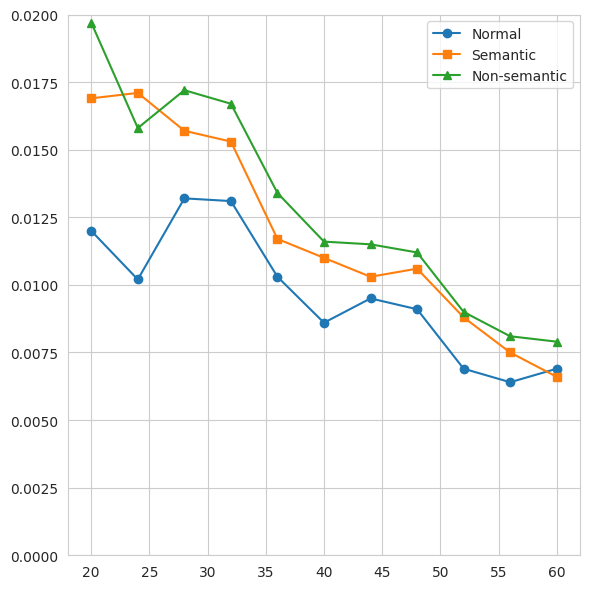
\includegraphics[width=\textwidth]{figures/rbad/assets/Synthesized Experiments/latest-eps=0.01, NNF-ratio=0.2, NRP-ratio=0.2, C-ratio=0.8, d-ratio=1.1.png}
        % \caption{$c_3 = 1.2$}
        % \label{fig-c_3=1.2}
    \end{subfigure}
    \hfill
    \begin{subfigure}[b]{0.3\textwidth}
        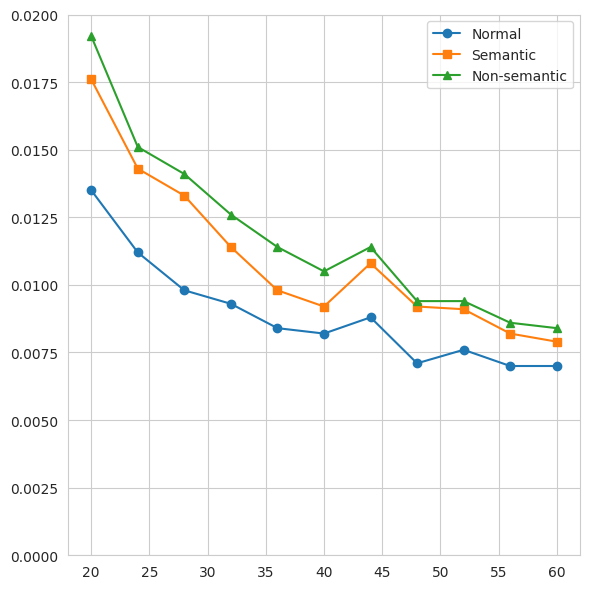
\includegraphics[width=\textwidth]{figures/rbad/assets/Synthesized Experiments/latest-eps=0.01, NNF-ratio=0.2, NRP-ratio=0.2, C-ratio=0.8, d-ratio=1.2.png}
        % \caption{$c_3 = 1.5$}
        % \label{fig-c_3=1.5}
    \end{subfigure}
    \hfill
    \begin{subfigure}[b]{0.3\textwidth}
        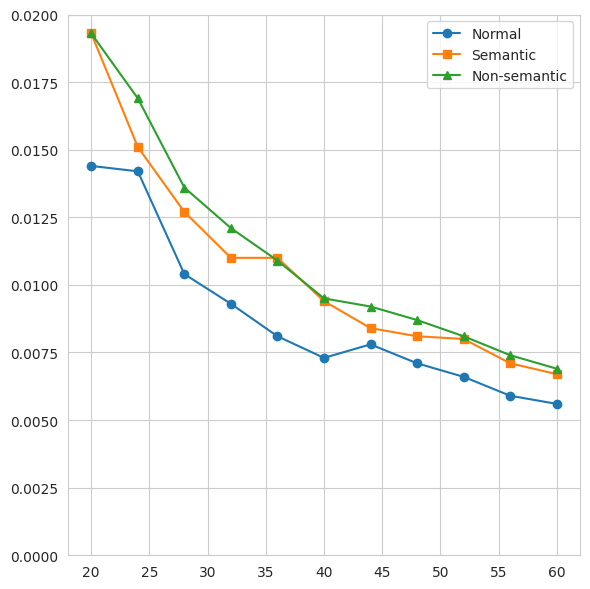
\includegraphics[width=\textwidth]{figures/rbad/assets/Synthesized Experiments/latest-eps=0.01, NNF-ratio=0.2, NRP-ratio=0.2, C-ratio=0.8, d-ratio=1.5.png}
        % \caption{$c_3 = 2$}
        % \label{fig-c_3=2}
    \end{subfigure}    
    \caption{Testing the under-parameterized setting with $C = {\rm{int}}(0.8P)$.
    {\color{red}
    By comparing to \ref{fig-synthesized-experiment-results}, this set of experimental results implies that slight over-parameterization (i.e., $C = {\rm{int}}(1.2P)$)could help the model better reconstruct all types of inputs.
    Here, we primarily compare the magnitudes of $P$ and $C$. 
    Specifically, the scenario where the ratio $C/P>1$ is referred to as \textit{over-parameterized}, while the converse (i.e., $C/P<1$) is defined as \textit{under-parameterized}.}
    }
    \label{fig-synthesized-experiment-results-under-parameterized}
\end{figure}

In \ref{sec-reconstruction}, we study the case when only one patch is replaced by the anomaly patch and claim that our analysis can be naturally extended to the case when multiple patches are replaced.
We consider the \textit{number of replaced patch} $\mathbf{NRP} = {\rm{int}}(c_4 P + 2)$ with $c_4 \in \{0, 0.1, 0.2\}$.
As demonstrated in \ref{fig-synthesized-experiment-results-NRP}, the gaps between the reconstruction errors of the normal data and the anomalies become significantly wider when more patches are replaced, which is consistent with our analysis.


\begin{figure}[H]
   \centering
   \begin{subfigure}[b]{0.3\textwidth}
      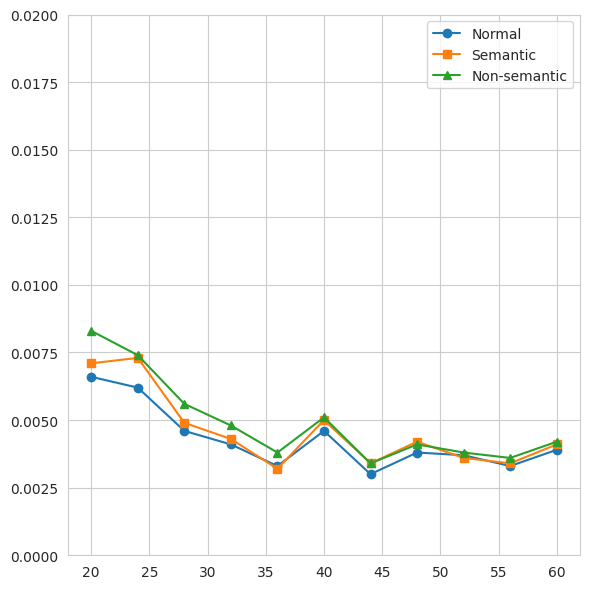
\includegraphics[width=\textwidth]{figures/rbad/assets/Synthesized Experiments/latest-eps=0.01, NNF-ratio=0, NRP-ratio=0, C-ratio=1.2, d-ratio=2.png}
      \caption{$c_4 = 0$}
      \label{fig-NRP=0}
   \end{subfigure}
   \hfill
   \begin{subfigure}[b]{0.3\textwidth}
      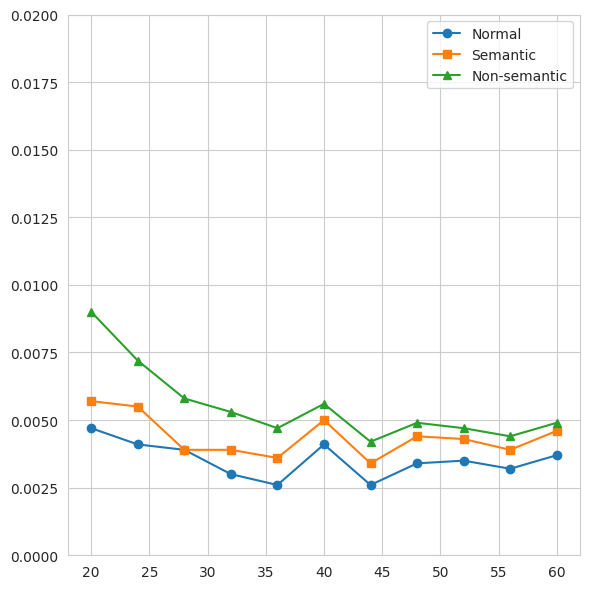
\includegraphics[width=\textwidth]{figures/rbad/assets/Synthesized Experiments/latest-eps=0.01, NNF-ratio=0.2, NRP-ratio=0.2, C-ratio=1.2, d-ratio=2.png}
      \caption{$c_4 = 0.2$}
      \label{fig-NRP=0.2}
   \end{subfigure}
   \hfill
   \begin{subfigure}[b]{0.3\textwidth}
      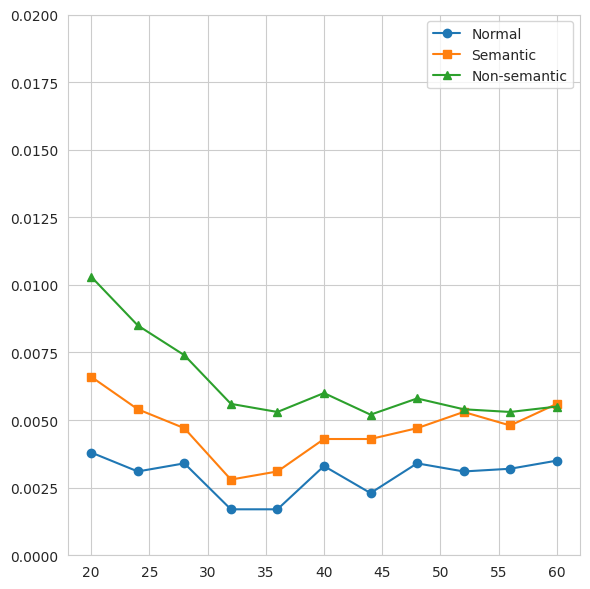
\includegraphics[width=\textwidth]{figures/rbad/assets/Synthesized Experiments/latest-eps=0.01, NNF-ratio=0.4, NRP-ratio=0, C-ratio=1.2, d-ratio=2.png}
      \caption{$c_4 = 0.4$}
      \label{fig-NRP=0.4}
   \end{subfigure}    
   \caption{Testing different numbers of replaced patches. 
   {\color{red}
   The parameter $c_4$ is used to characterize the number of patches replaced in anomalies, where a larger $c_4$ indicates a greater number of replaced patches.
   The gaps between the reconstruction errors of the normal data and the anomalies become significantly wider when more patches are replaced, which is consistent with our analysis.}}
   \label{fig-synthesized-experiment-results-NRP}
\end{figure}

\newpage

{\color{red}
\subsubsection{The Growth of the Norm of the Kernels}\label{sec-kernel-norm-growth-experiments}

This section reports the growth of the norm of the kernels during training. 
According to \ref{lemma-size-of-wj-in-paper}, the growth rates of the norm of the kernels is upper bounded by \ref{eq-lemma-size-of-wj-random-initialization-in-paper,eq-lemma-size-of-wj-result-2-in-paper}.
As a side product of the synthesized experiments in \ref{sec-experiments-detail}, we record the norm of the kernels during training.
The results are presented in Figures \ref{fig-inner-product-kernels-features-1} - \ref{fig-inner-product-kernels-features-6}.
In all the experiments, the norm of the kernels increases almost linearly, which is consistent with our analysis in \ref{eq-lemma-size-of-wj-random-initialization-in-paper,eq-lemma-size-of-wj-result-2-in-paper}. 
Additionally, kernels with larger initial values grow faster. 
It can be observed that as the number of kernels and patches increases (i.e., when the task becomes more complex), the differences between kernels also become more pronounced.
The discussion of the results can be found in Remark \ref{remark-discussion-aux-experiments}

\subsubsection{Inner Product between the Kernels and the Features}\label{sec-inner-product-experiments}

A key observation underlying our proposed cone set intuition is that kernels tend to converge toward features in terms of direction, which can be measured by the (normalized) inner product between the kernels and the features.
We report the inner products between the kernels and the features during training in c
The discussion of the results can be found in Remark \ref{remark-discussion-aux-experiments}

\newpage

\begin{figure}[H]
    \centering
    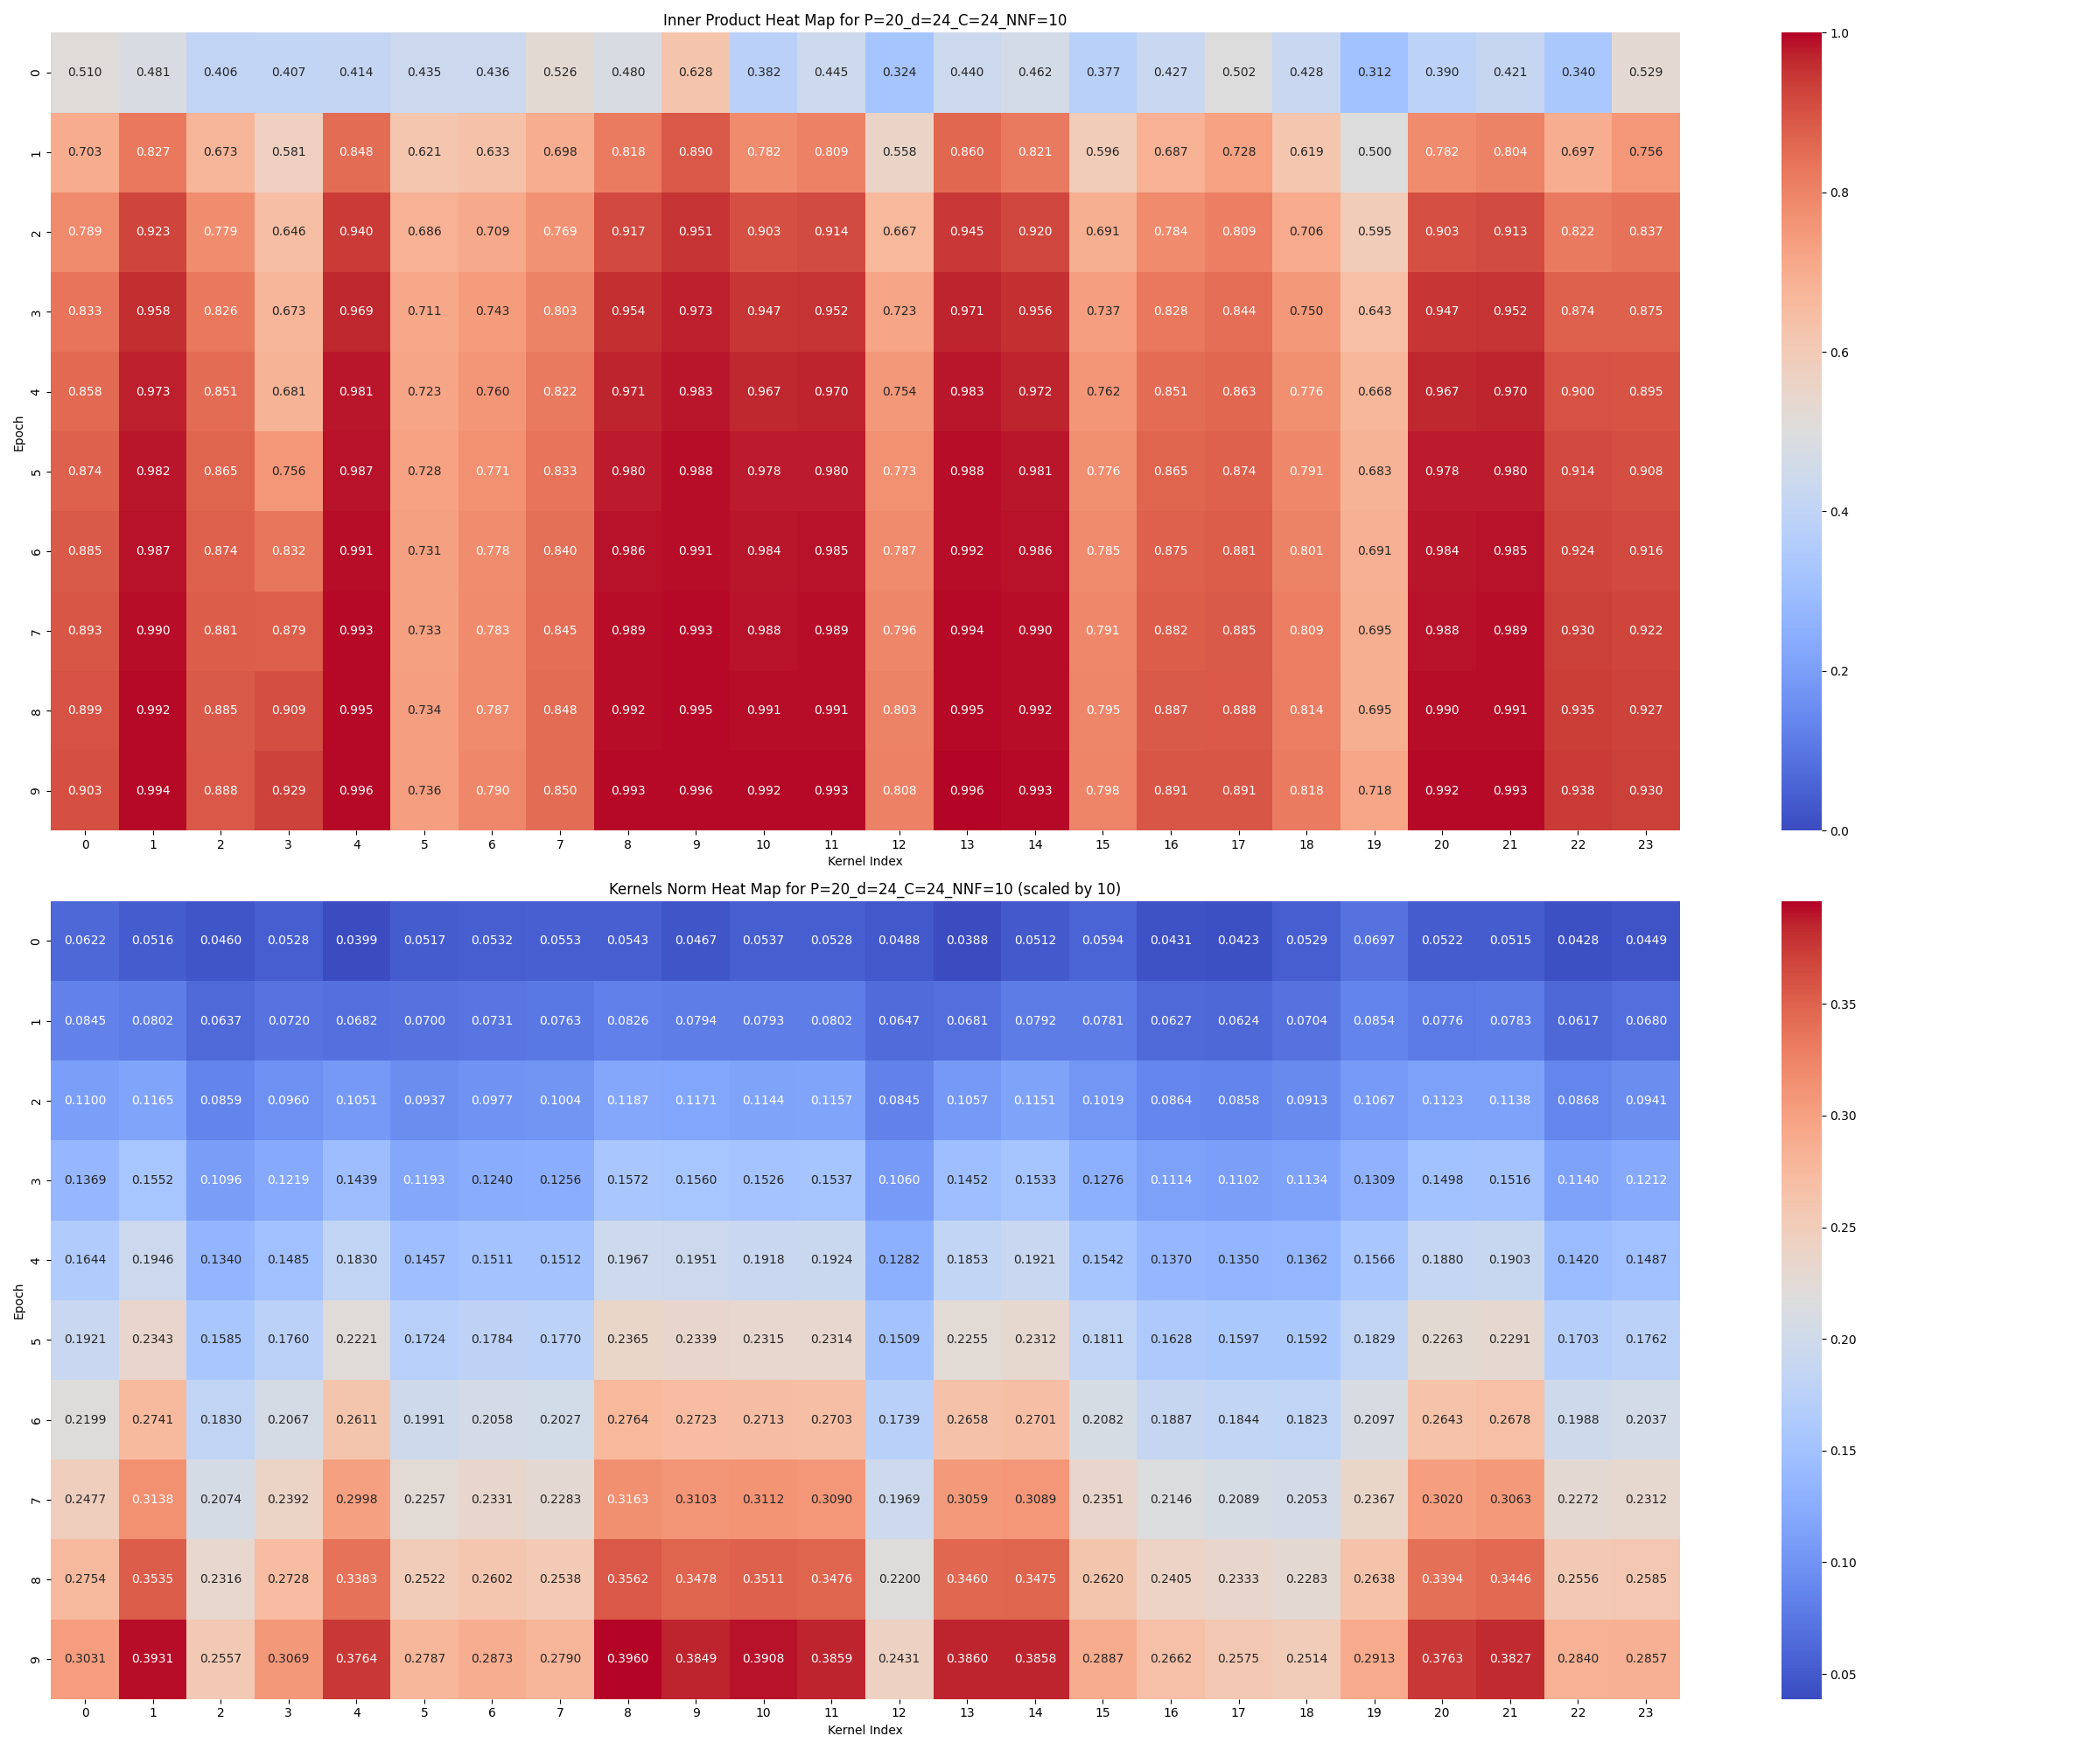
\includegraphics[width=\textwidth]{figures/rbad/figs/P=20_d=24_C=24_NNF=10.png}
    \caption{
    {\color{red}
    Recorded \textbf{kernels' norm} (the \textit{below} sub-figure) and \textbf{inner products between the kernels and the features} (the \textit{above} sub-figure) during training.
    The controling variables are $P=20, d=24$, and $C=24$.
    In both sub-figures, the $x$-axis represents the kernel index $j$ ($j \in [C]$), and the $y$-axis denotes the training epoch.
    For better visualization, we have scaled the norm of the kernels by a factor of 10 in the below sub-figure.
    }}
    \label{fig-inner-product-kernels-features-1}
\end{figure}

\begin{figure}[H]
    \centering
    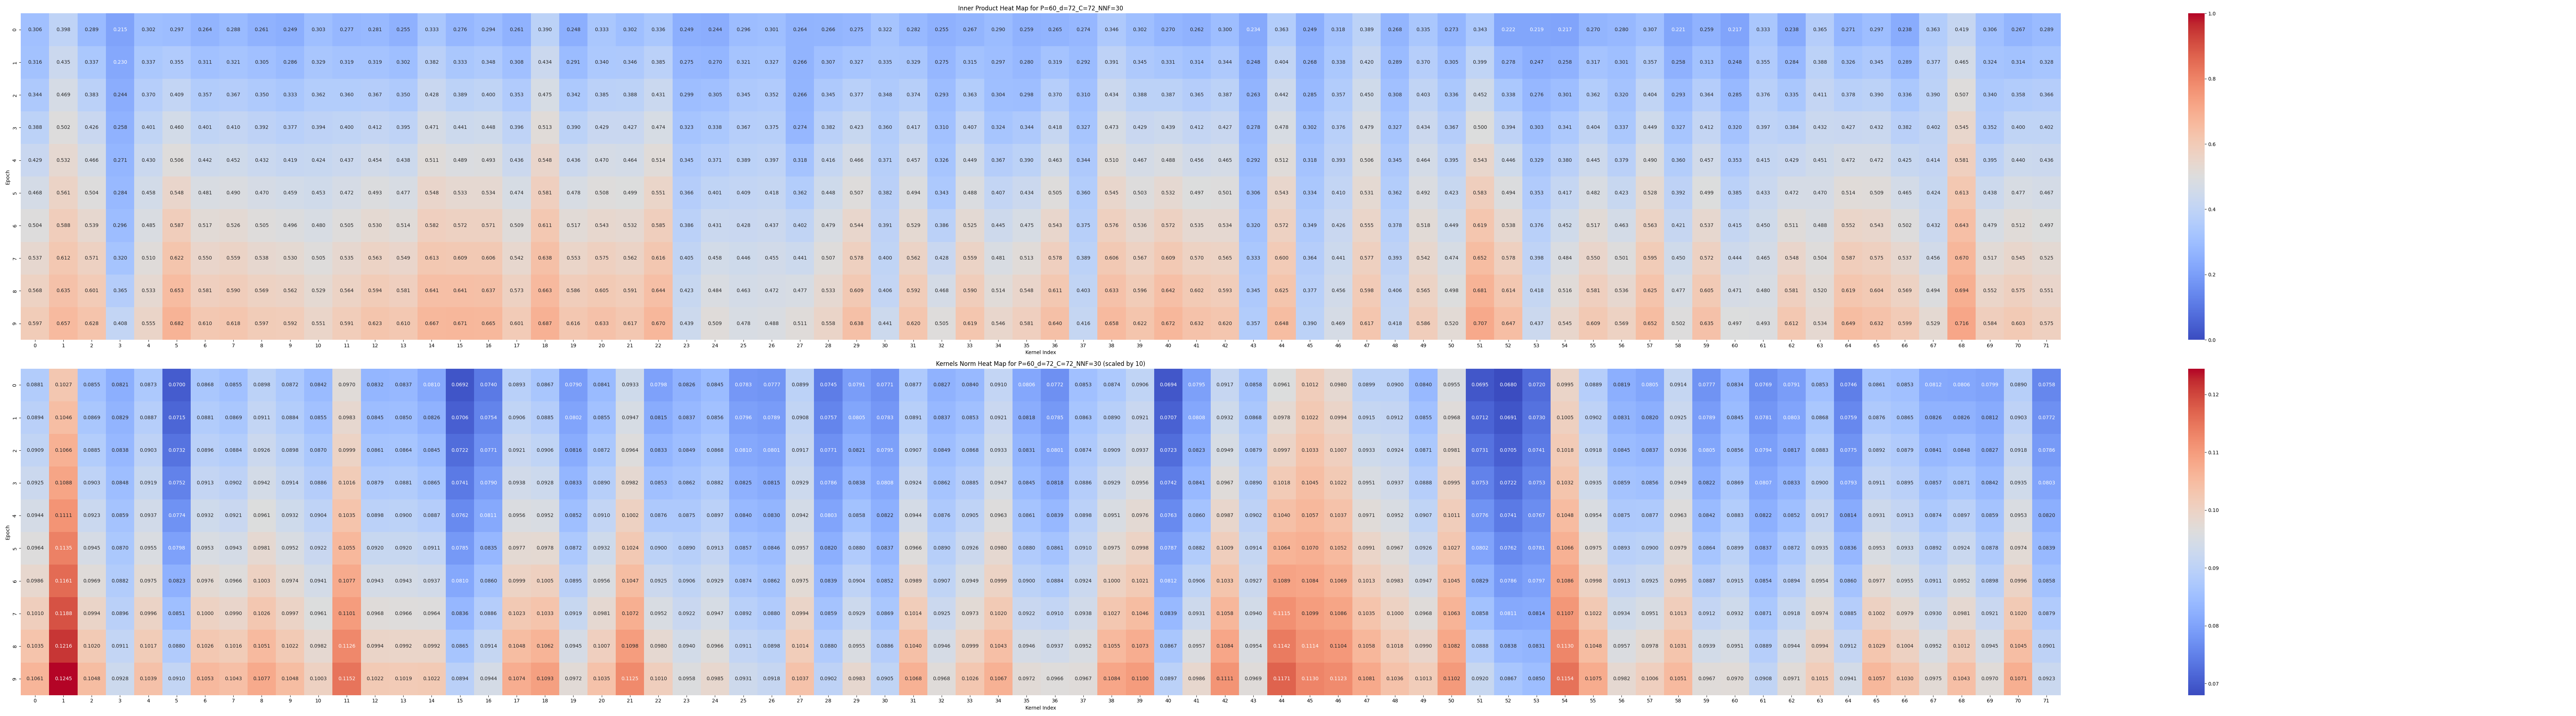
\includegraphics[width=\textwidth]{figures/rbad/figs/P=60_d=72_C=72_NNF=30.png}
    \caption{{\color{red}The control variables are $P=60, d=72,$ and $C=72$.}}
    \label{fig-inner-product-kernels-features-2}
\end{figure}

\begin{remark}[Discussions on the results in \ref{sec-inner-product-experiments,sec-kernel-norm-growth-experiments}]
\label{remark-discussion-aux-experiments}
An intuitive observation is that the color of each column (representing one single kernel) becomes progressively warmer from top to bottom in both sub-figures, which implies that both the norm and the inner product increase with the training epoch.
In particular, the growth of the inner product can serve as an evidence for our proposed cone set intuition, i.e., the kernels tend to converge toward features in terms of direction.

The main difference between Figures \ref{fig-inner-product-kernels-features-1} - \ref{fig-inner-product-kernels-features-6} lies in the controling variables $P, d,$ and $C$, which depict different levels of task complexity.
As the dimension increases, randomly initialized kernels become more difficult to be absorbed (reflected in the bound provided by \ref{theorem-initial-size-in-paper}).
Figures \ref{fig-inner-product-kernels-features-3} - \ref{fig-inner-product-kernels-features-6} provide more experimental results.
The similar captions are omitted for brevity.

\end{remark}

\begin{figure}[H]
    \centering
    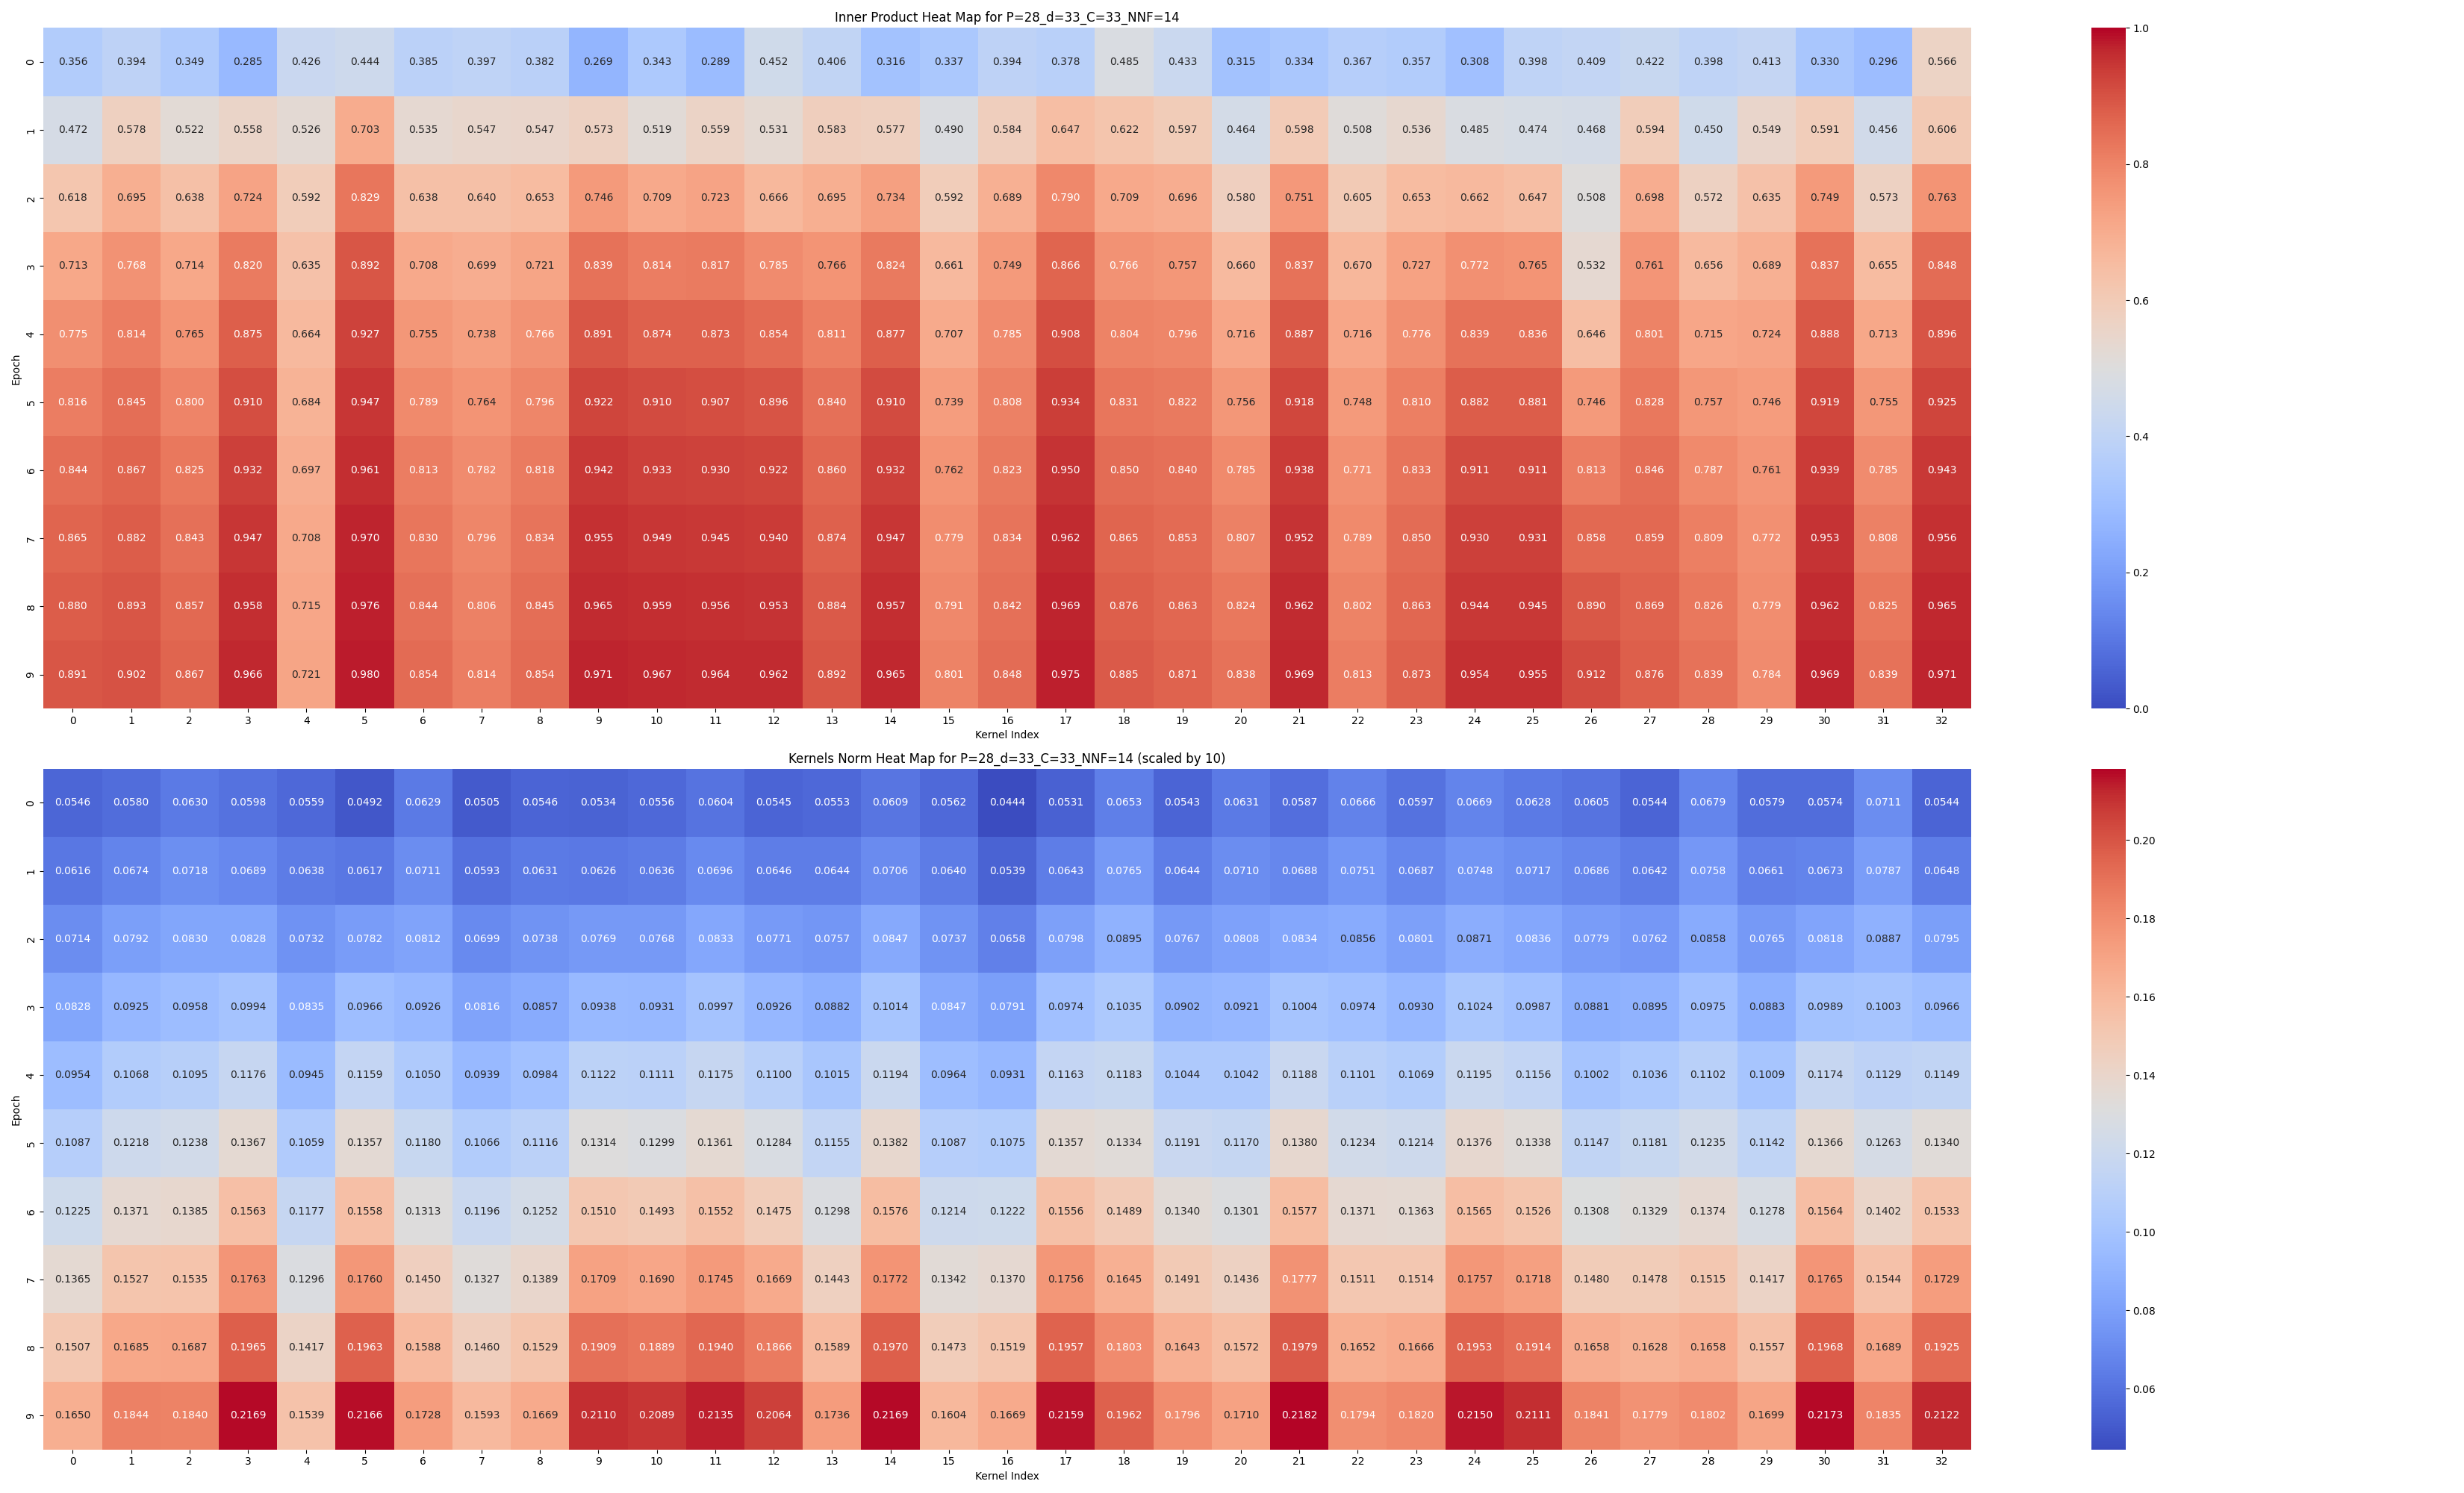
\includegraphics[width=\textwidth]{figures/rbad/figs/P=28_d=33_C=33_NNF=14.png}
    \caption{
        {\color{red}The control variables are $P=28, d=33,$ and $C=33$.}}
    \label{fig-inner-product-kernels-features-3}
\end{figure}

\begin{figure}[H]
    \centering
    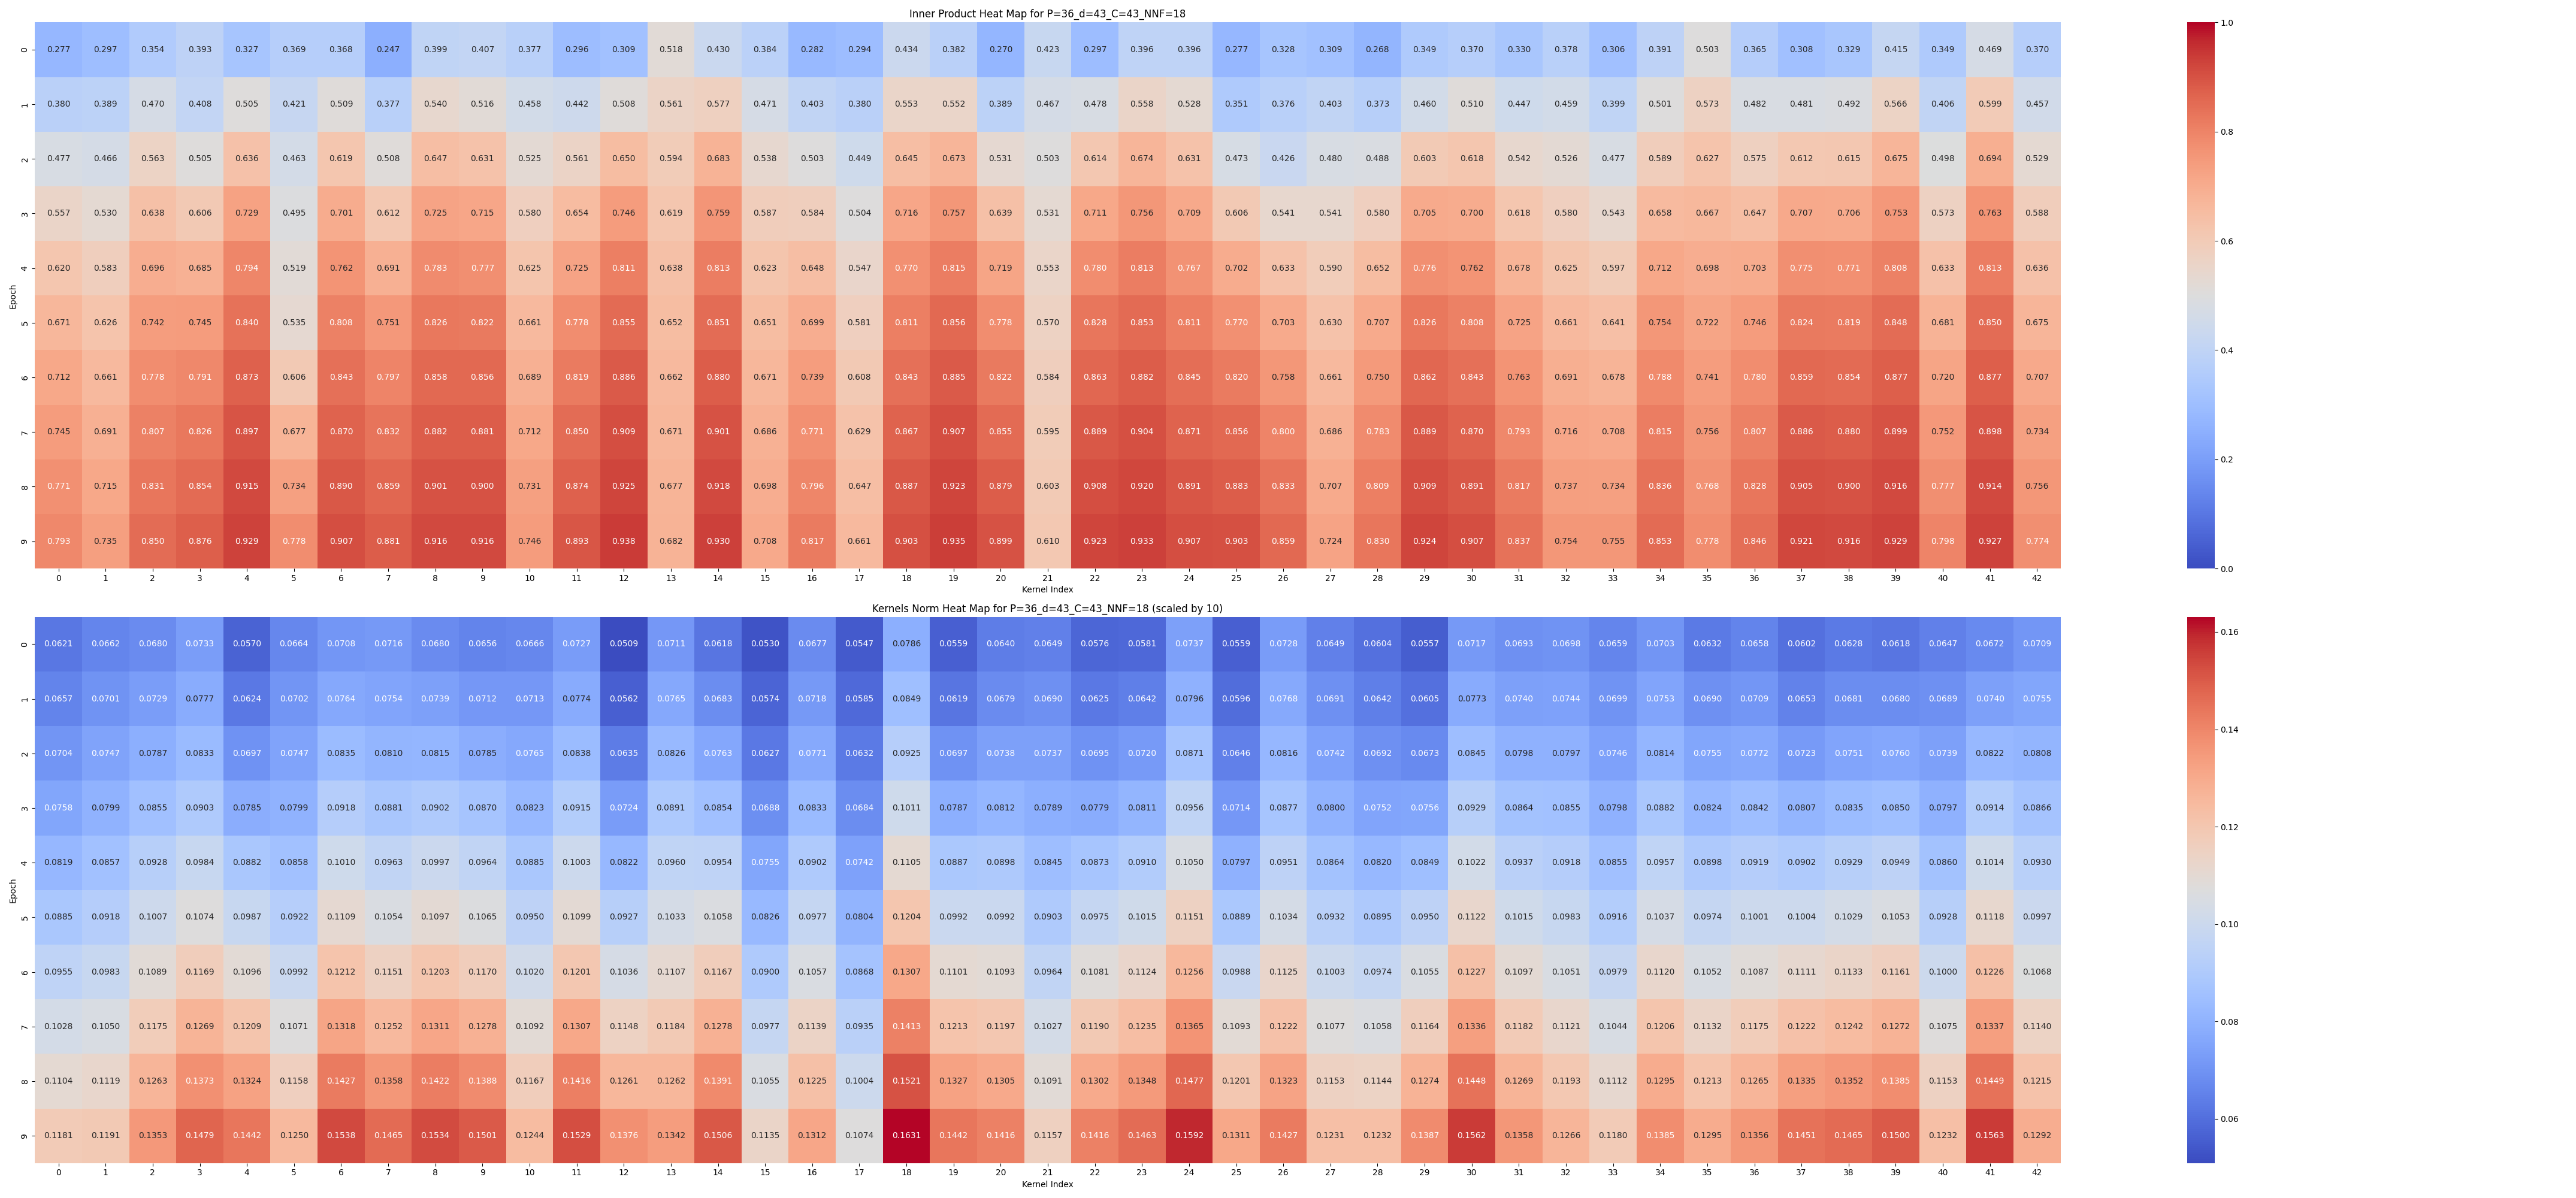
\includegraphics[width=\textwidth]{figures/rbad/figs/P=36_d=43_C=43_NNF=18.png}
    \caption{{\color{red}The control variables are $P=36, d=43,$ and $C=43$.}}
    \label{fig-inner-product-kernels-features-4}
\end{figure}

\begin{figure}[H]
    \centering
    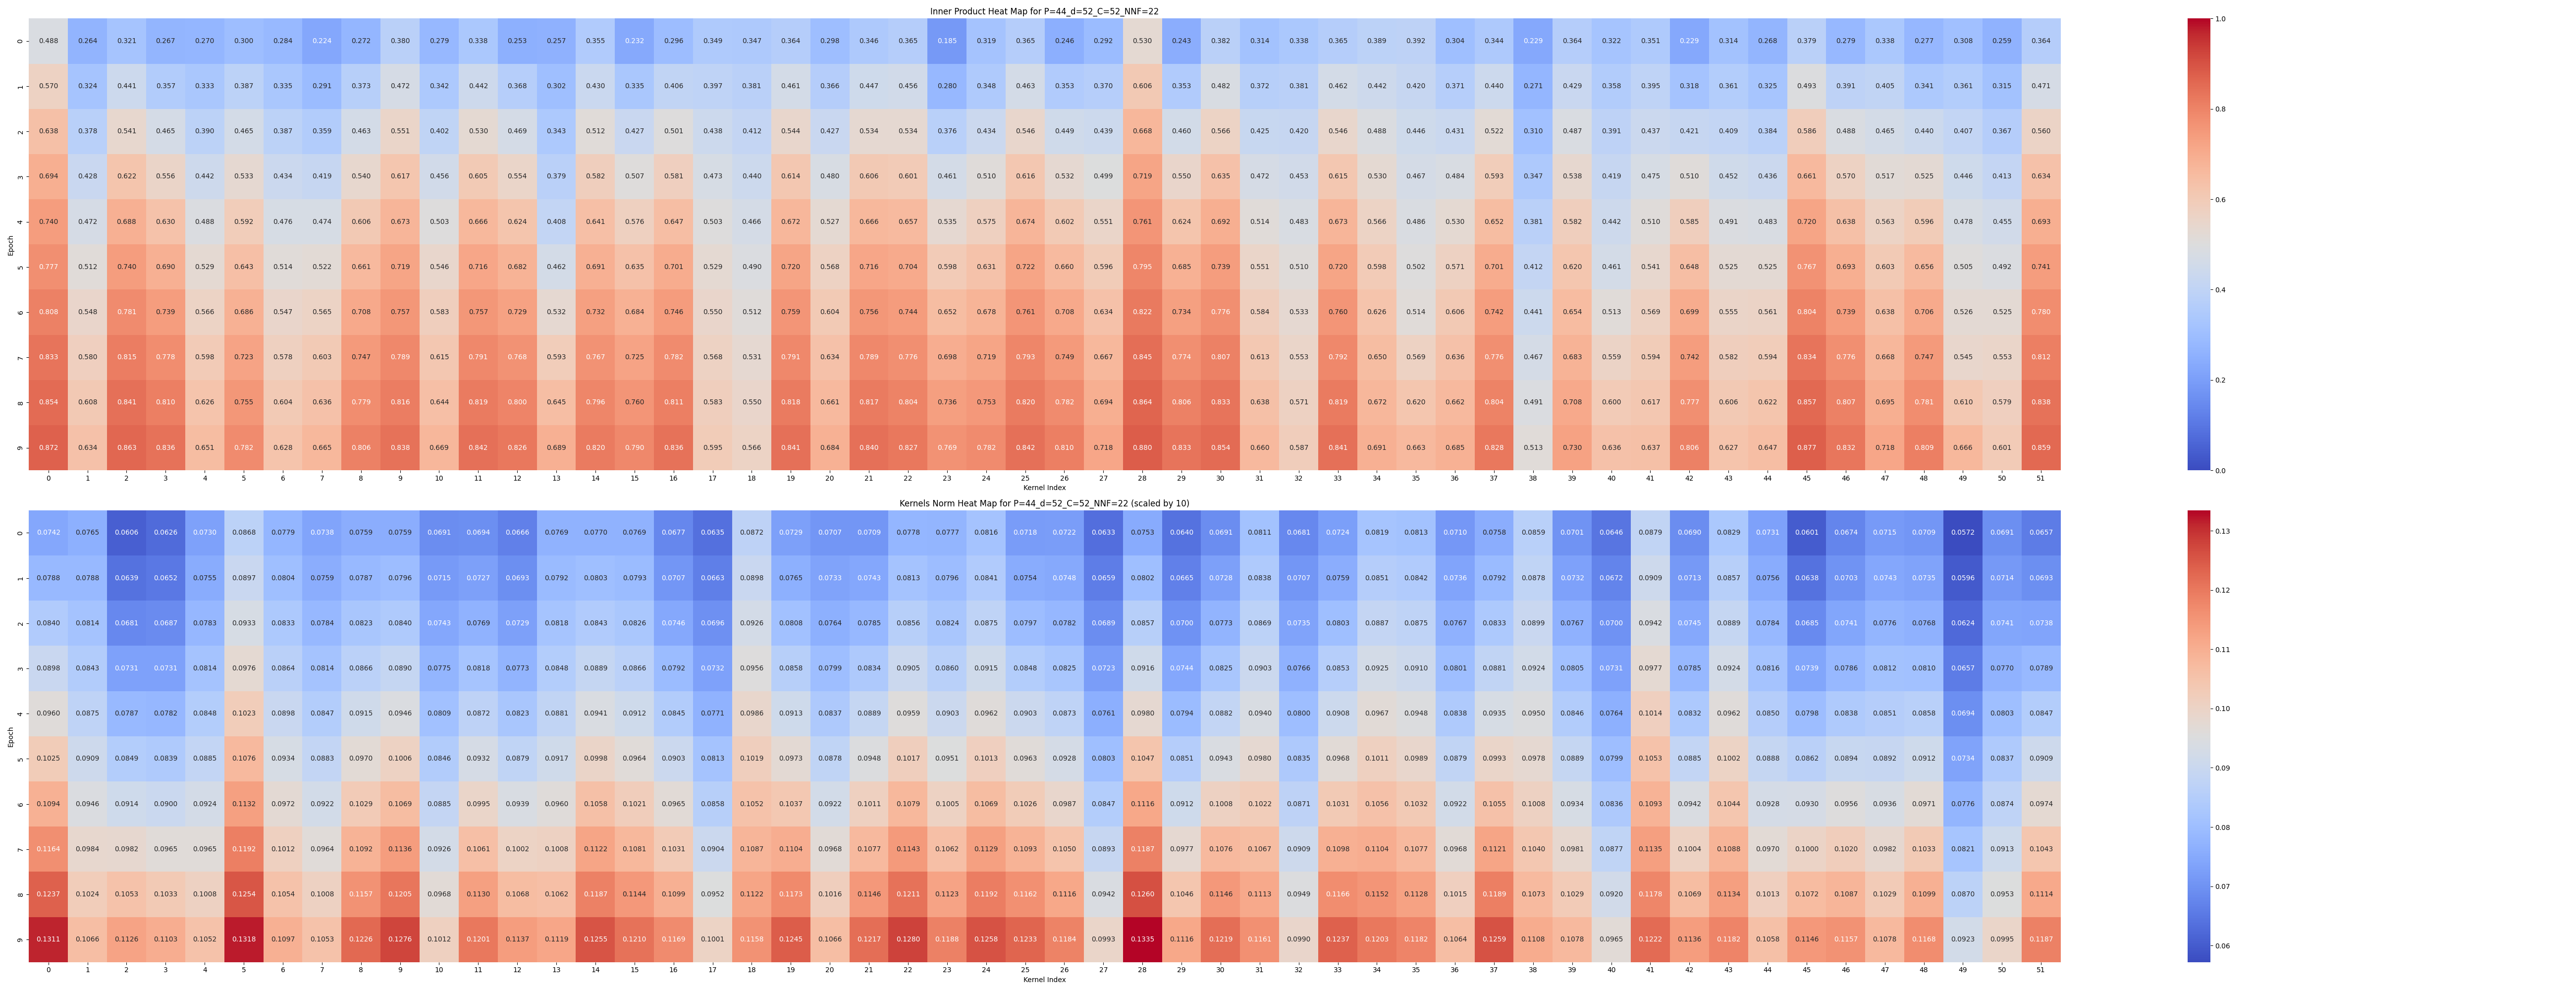
\includegraphics[width=\textwidth]{figures/rbad/figs/P=44_d=52_C=52_NNF=22.png}
    \caption{{\color{red}The control variables are $P=44, d=52,$ and $C=52$.}}
    \label{fig-inner-product-kernels-features-5}
\end{figure}

\begin{figure}[H]
    \centering
    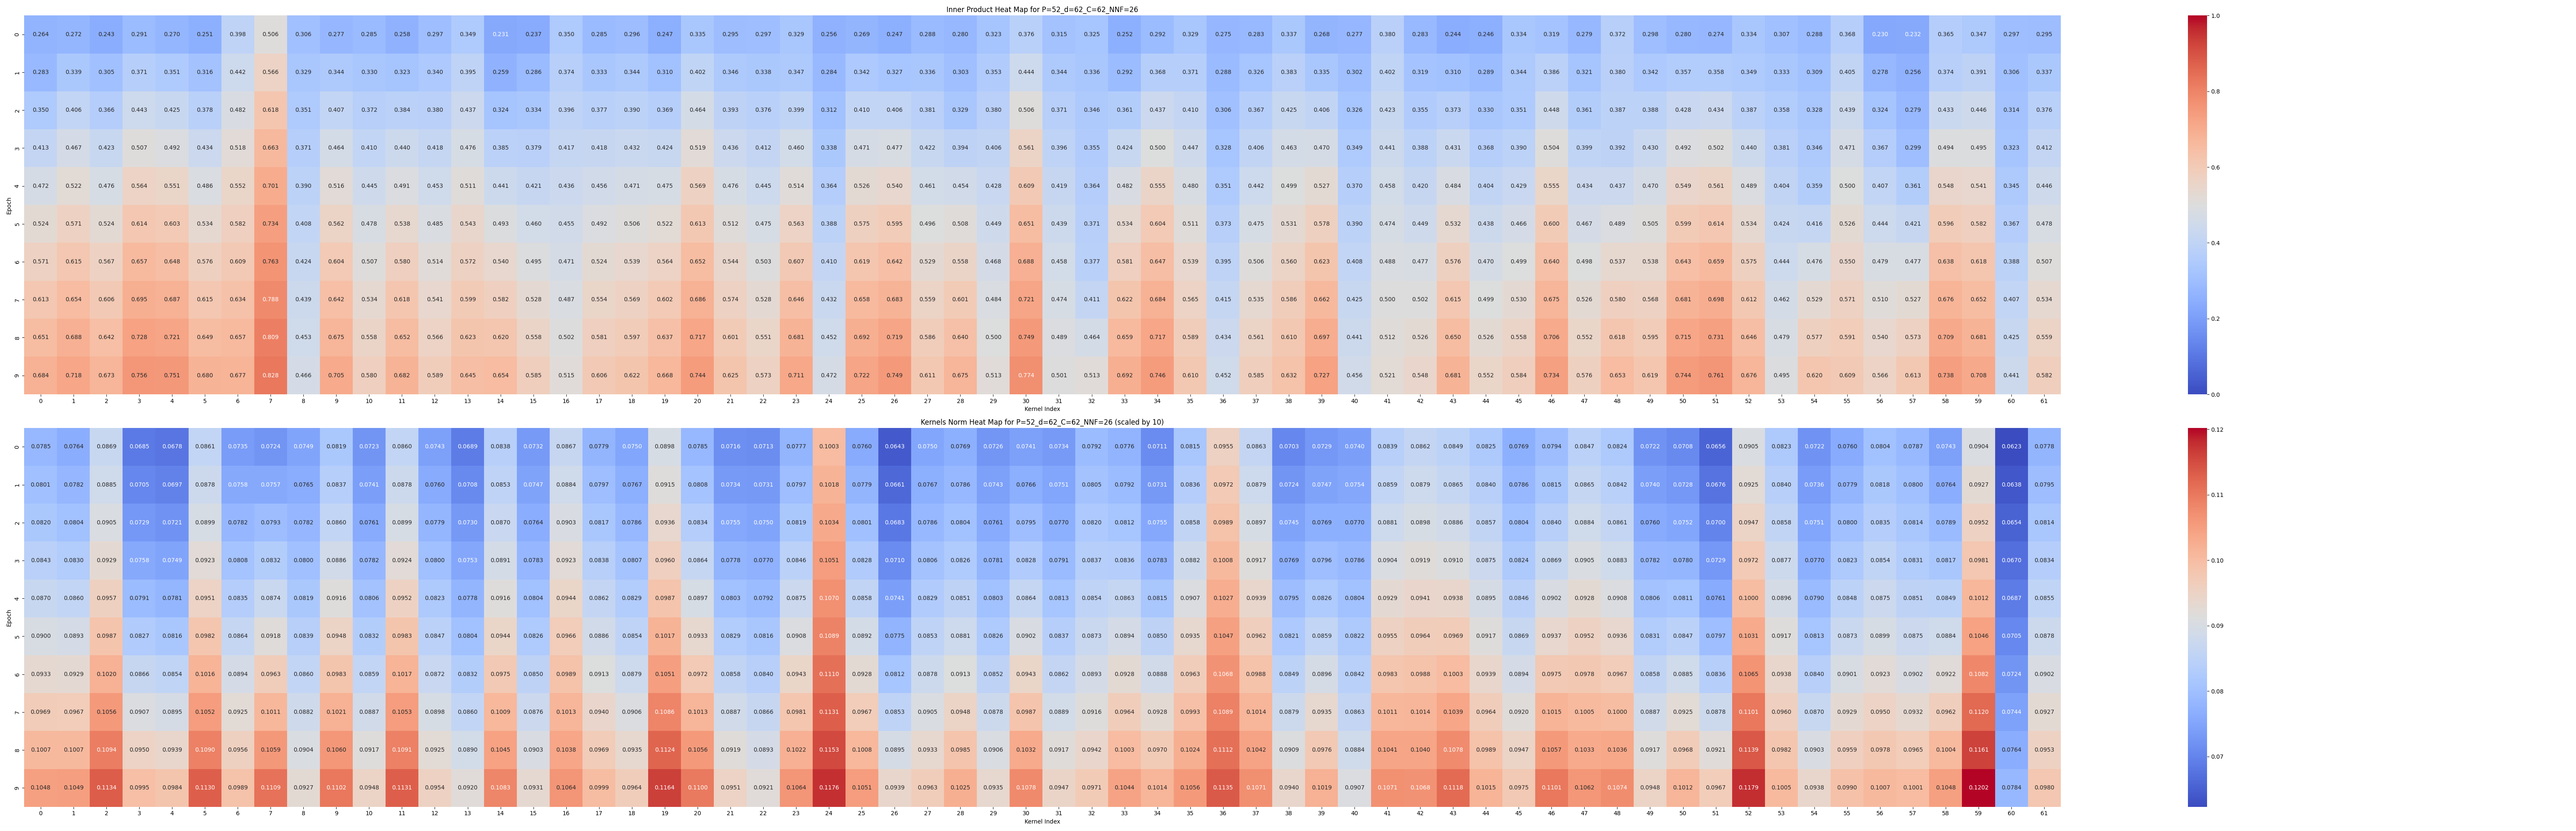
\includegraphics[width=\textwidth]{figures/rbad/figs/P=52_d=62_C=62_NNF=26.png}
    \caption{{\color{red}The control variables are $P=52, d=62,$ and $C=62$.}}
    \label{fig-inner-product-kernels-features-6}
\end{figure}
}